\documentclass[a4paper,11pt]{ltjsarticle}

% ========== package ========== %
% --- 数式環境 --- %
\usepackage{amsmath}
\usepackage{amssymb}
\usepackage{mathtools}
% --- 数式環境 END --- %
% ブラケット
\usepackage{braket}
% ベクトルの太文字
\usepackage{bm}
% 添え字左右上下 \fourIdx{左上}{左下}{右上}{右下}{ベース} で使う．Iは大文字
\usepackage{fouridx}
% 色
\usepackage{color}
% 余白指定
\usepackage{geometry}
% --- ページ内リンク --- %
\usepackage{hyperref}
\hypersetup{colorlinks=true,linkcolor=blue}
% --- ページ内リンク END --- %
% 花文字
\usepackage{mathrsfs}
% 画像
\usepackage{graphicx}
% tcolorbox
\usepackage{tcolorbox}
% appendix
\usepackage{appendix}
% --- 参考文献 --- %
\usepackage{etoolbox}
\usepackage{fontspec} % fontspecは読み込んでOKですが、設定順序に注意が必要です
%% --- 参考文献フォント --- %%
  \IfFontExistsTF{Times New Roman}{
    \newfontfamily\bibfontface{Times New Roman}
  }{
    \newfontfamily\bibfontface{FreeSerif} % 代替フォント
  }
%% --- 参考文献フォント END --- %%
%% --- 参考文献リンク位置 --- %%
  \BeforeBeginEnvironment{thebibliography}{%
    \phantomsection
    \addcontentsline{toc}{section}{参考文献}
  }
  \AtBeginEnvironment{thebibliography}{%
    \normalfont\bibfontface
    \addfontfeatures{Ligatures=TeX}%
  }
%% --- 参考文献のリンク位置 --- %%
% --- 参考文献 END --- %
% ========== package END ========== %

% ========== newcommand ========== %
% --- セクションから目次へのリンク --- %
\newcommand{\sectionlink}[1]{\section[#1]{\hyperlink{toc}{#1}}}
\newcommand{\subsectionlink}[1]{\subsection[#1]{\hyperlink{toc}{#1}}}
% セクション番号リンク
\makeatletter
\renewcommand{\@seccntformat}[1]{%
  \protect\hyperlink{toc}{\csname the#1\endcsname}\quad
}
\makeatother

\numberwithin{equation}{section}
% ==========- newcommand END ========== %
\allowdisplaybreaks
%===========================================================
% --- タイトル --- %
%===========================================================
\geometry{left=25mm, right=25mm, top=30mm, bottom=30mm}

% 原文の図版・演習枠・記号を再現するための追加設定
\usepackage{xcolor}
\usepackage{feynmp}
\usepackage{slashed}
\usepackage{subfigure}
\usepackage{booktabs}
\usepackage[framemethod=default]{mdframed}
\definecolor{lightgray}{gray}{0.9}
\newmdenv[skipabove=10pt,skipbelow=10pt,
rightline=false,leftline=false,topline=false,bottomline=false,
backgroundcolor=gray!20,linecolor=gray,
innerleftmargin=10pt,innerrightmargin=10pt,
innertopmargin=10pt,innerbottommargin=10pt,
leftmargin=0cm,rightmargin=0cm,linewidth=4pt]{eBox}
\def\be{\begin{equation}}
\def\ee{\end{equation}}
\def\ba{\begin{eqnarray}}
\def\ea{\end{eqnarray}}
\def\bi{\begin{itemize}}
\def\ei{\end{itemize}}
\def\l{\left}
\def\r{\right}
\def\fr{\frac}
\def\la{\label}
\def\d{\partial}
\def\vphi{\varphi}
\def\pr{\prime}
\def\mpl{M_{\rm p}}
\def\hub{\mathcal{H}}
\def\mbf{\mathbf}
\newcommand{\high}[1]{\underline{\emph{#1}}}
\DeclareGraphicsRule{*}{mps}{*}{}
% 原文は節によらない通し式番号を採用している。
\counterwithout{equation}{section}
\renewcommand{\theequation}{\arabic{equation}}
\hypersetup{pdftitle={有効場の理論入門 (arXiv:2006.16285v1 日本語訳)},
pdfauthor={Riccardo Penco},citecolor=blue,urlcolor=blue}
\title{\bfseries 有効場の理論入門\\[0.4em]
\large An Introduction to Effective Field Theories\\[0.4em]
\normalsize \href{https://arxiv.org/pdf/2006.16285v1}{arXiv:2006.16285v1}（日本語訳）}
\author{Riccardo Penco\thanks{コメントや訂正は \texttt{rpenco@cmu.edu} までお寄せいただきたい。}}
\date{{\small Department of Physics, Carnegie Mellon University, Pittsburgh, PA}\\[1em]
2020年7月1日}
% 参考文献の最初・最後の1行だけを別ページに残さない。
\apptocmd{\thebibliography}{\clubpenalty=10000\widowpenalty=10000\interlinepenalty=10000}{}{}
\begin{document}
\begin{fmffile}{graphs}
\maketitle
\begin{abstract}
本講義ノートは、有効場の理論（EFT）の方法を概観するものである。
EFTのトイモデル、カイラル摂動論、Fermi液体論、非相対論的QEDを取り上げ、
これらの例を用いて、ツリーレベルおよびループレベルでのマッチング、
大きな対数の総和、自然性の問題、スプリオン場、剰余空間構成、
Wess-Zumino-Witten項、カイラルアノマリーとゲージアノマリー、
場の位相の再定義、領域展開法など、さまざまなEFTの概念を導入する。
この講義ノートは、2020年6月22日から7月3日までBrazilのSao Pauloで開催された
第2回Joint ICTP-Trieste/ICTP-SAIFR素粒子物理学スクールのために作成された。
\end{abstract}
\clearpage
\hypertarget{toc}{}
\tableofcontents
\clearpage
\nocite{Srednicki:2007ab,Wilson:1993dy,Georgi:1991ch,Weinberg:1995mt,tHooft:1979bh,Goon:2016ihr,Adams:2006sv,Vafa:2005ui,Weinberg:1987dv,Alberte:2016izw,Graham:2019bfu,Georgi:1994qn,Manohar:1996cq,Pich:1998xt,Rothstein:2003mp,Kaplan:2005es,Burgess:2007pt,Skiba:2010xn,Gripaios:2015qya,Petrov:2016azi,Manohar:2018aog,Cohen:2019wxr,Dine:2015xga,Giudice:2017pzm,Weinberg:1988cp,Weinberg:1981qq,Scherer:2002tk,Callan:1969sn,Volkov:1973vd,ogievetsky:1974ab,Weinberg:1996kr,Carroll:2004st,Witten:1983tw,Goon:2012dy,Harvey:2005it,Preskill:1990fr,Ecker:1994gg,Pich:1995bw,Burgess:1998ku,Pich:2018ltt,Bilal:2008qx,Zee:2003mt,Shankar:1993pf,Jackson:1998nia,Griesshammer:1997wz,Goldberger:2007hy,Porto:2016pyg,Labelle:1996en,Grinstein:1997gv,Polchinski:1992ed,Leggett:1975te,Caswell:1985ui}
\sectionlink{はじめに}




自然についての注目すべき事実は、興味深い現象が、エネルギー・長さ・時間の広い範囲のスケールにわたって生じることである。この一世紀だけでも、私たちは研究の対象を、原子の大きさの10億分の1ほどの微視的スケール（$10^4$ GeV）から、観測可能な宇宙の大きさに及ぶ巨視的スケール（$10^{-42}$ GeV）まで広げてきた。この巨大なエネルギー範囲こそが、物理科学の成功の鍵である。もしすべての物理現象が同じスケールで起きていたなら、それらを一度にすべて理解しなければならなかっただろう。物理学の進歩は不可能だったはずである！　実際には、このスケールの分離を利用して、関心のある物理過程の典型的エネルギー$E$よりはるかに大きい（小さい）スケールを、第一近似としてすべて無限大（ゼロ）に置くことができる。この極限では、$E$と大きく異なるスケールの物理は無関係となり、無視できる。必要なら、その影響を摂動論で再び取り入れればよい。この基本戦略は、今日に至るまで、あらゆる分野の物理学者によって、多かれ少なかれ暗黙のうちに採用されている。

有効場の理論（EFT）は、上で述べた戦略を明示的に実装し、精密で定量的な枠組みにするための模型構築の道具である。素粒子物理学者はエネルギースケールで考えることを好むが、EFTは、長さ、時間、速度、運動量、角運動量など、あらゆる種類の次元をもつ量の間の階層性を利用して構築できる。実際、適切に定式化すれば、次のようにまで主張できる。
\vspace{.3cm}
%
\begin{quotation}
\noindent \hspace{3cm} {\it すべての物理理論は有効理論である。}
\end{quotation}
%
\vspace{.3cm}

以下では、EFTの主要な道具のいくつかを、さまざまな状況でどのように働くかを示しながら紹介する。本講義ノートは、高エネルギー物理学の基礎知識をもつ大学院生や若手の博士研究員を対象としている。実際、私が大学院生だったときに読みたかったと思うノートを書くことを目指した。したがって、内容の大部分はEFTを使い慣れた読者には既知だろうが、そのような読者にも、ところどころに有益な点を見いだしてもらえれば幸いである。


\subsectionlink{EFTの主要な構成要素}


本講義では、Wilsonによる繰り込み群（RG）へのアプローチの議論から始めるような、歴史的な順序には従わない。主要な原理は非常に簡単に述べられるので、ただちに本題に入り、EFTについての現在の理解を手短にまとめる。EFTは有効作用によって定義され、その有効作用は次の三つの要素によって完全に指定される。
%
\begin{enumerate}
\item {\it 自由度。} EFTを構築する際の第一歩は、関心のある物理系を記述するうえで、どの自由度が重要かを見極めることである。これらが有効作用に現れる変数になる。ここでの鍵は「重要な」という言葉である。追加の構造を導入すれば、どんな現象の記述もいくらでも複雑にできるが、その見返りはすぐに小さくなる。逆に、最も簡潔な記述を目指すこともできるが、Albert Einsteinの言葉を借りれば、{\it 「すべては可能な限り単純にすべきだが、それ以上単純にしてはならない」}。Nambu-Goldstoneモードの場合のように、用いるべき自由度が対称性の考察から示唆されることもある。しかし、多くの場合、自由度の選択は独立した入力であり、科学であると同時に技でもある。
\item {\it 対称性。} EFTを構築する第二段階は、有効作用の形、ひいては系の力学を制約する対称性を特定することである。対称性には、大域的なもの、ゲージ化されたもの、偶発的なもの、自発的に破れたもの、量子異常をもつもの、近似的なもの、縮約されたものなど、さまざまな種類がある。これらすべての例を、順を追って見ていく。ここでは、系の対称性と両立する項は、原理的にはすべて有効作用に含めるべきだとだけ述べておく。その結果、有効作用は一般に無限個の項を含む。
\item {\it 展開パラメータ。} 無限個の項をもつ作用を扱う鍵は、すべてのEFTが一つ以上の展開パラメータを備えているという事実にある。これらは、無視することにした物理が、残すことにした自由度に及ぼしうる影響を制御する小さな量である。例えば素粒子物理学では、これらの展開パラメータはしばしばエネルギースケールの比$E / \Lambda$であり、$E$は関心のある過程の特徴的なエネルギースケール、$\Lambda$は無視する紫外（UV）物理の典型的なエネルギースケールである。他の例としては、速度の比（例えば非相対論的極限での$v/c$）、角運動量の比（半古典的展開の場合）、あるいは小さな無次元結合定数が挙げられる。観測量は、これらの小さなパラメータについての級数として摂動論で計算する。この戦略が機能するには、明示的なパワーカウンティングの方式をもつことが不可欠である。すなわち、有効作用の各項に、展開パラメータについての明確な次数を割り当てられなければならない。これによって、摂動論の任意の次数で寄与する項が有限個に限られ、また、求める精度に応じて作用に残す項をあらかじめ決められることが保証される。
\end{enumerate}
%

これら三つの要素を述べることは比較的容易だが、EFTにそれらを正しく実装するには、微妙な注意が必要になることがある。それを実際にどう実現するかは、扱う問題に依存することが多い。この半世紀の間に豊富なノウハウが蓄積されてきた。本講義ノートの目的は、その主要な手法を紹介することである。



\subsectionlink{EFTの主な利点}


より根本的な理論が存在しないため、物理系のEFTによる記述に頼らざるをえない場合がある。また、そのような理論が存在しても、例えば強結合であるために、厳密な予言はおろか近似的な予言を引き出すことすら難しい場合もある。このような状況では、EFTは同じ物理について、より扱いやすい弱結合の記述を与えうる。さらに、必要に迫られてEFTを使う場合でなくても、EFTは便利な枠組みである。EFTのアプローチの主な利点は、次のようにまとめられる。
%
\begin{itemize}
\item EFTは、重要な自由度に焦点を絞り、扱う問題にとって重要でない側面を最初から無視することで、計算を大幅に簡単にする。
\item 重要な自由度を取り出すと、それまでは隠れていた新たな対称性が明らかになることがある。多くの場合、こうした対称性を用いると、ほとんど計算せずに、あるいはまったく計算せずに、一般的な結論を導ける。
\item EFTを用いると、計算は本質的に二つの部分に分離される。一つは残しておく自由度を含む部分（実際のEFTの計算）であり、もう一つは無視する物理に依存する部分（マッチング計算）である。この「モジュール化された」アプローチによって、同じような計算を何度も繰り返すことを避けられる。
\item 異なるスケールをいくつも含む問題では、それらの比の対数に依存する観測量が現れることがある。スケールが大きく離れていると、対数は大きくなり、摂動計算の精度を悪化させうる。EFTは一度に一つのスケールに注目することで、RGによる走りを使って、これらの大きな対数を足し上げられる。
\item EFTには、無視した物理の系統的なパラメータ表示が含まれる。その物理が未知であったり、十分に理解されていなかったりする場合でも、EFTの予言を実験と比較することで、模型に依存しない制約を課せる。
\item EFTの観測量は、一つ以上の展開パラメータに関する級数である。摂動論をどこまで進めるかによって、EFTの結果の精度が決まる。
\item これに関連して、EFTは、その予言をいつ信頼するのをやめるべきかまで教えてくれる。展開パラメータが$\mathcal{O}(1)$になる領域に入ると、摂動論は機能しなくなる。これは、それまで使っていた自由度がもはや重要な自由度ではなくなり、別のEFTを考える必要があることを意味する。
\end{itemize}
%
ここまでの指摘の中には、現時点では少しわかりにくく感じられるものもあるかもしれない。その場合は、このまま読み進め、EFTの例をいくつか見た後で、この小節に戻ってほしい。 \\

\noindent {\it 規約：} 特に断らない限り、文献~\cite{Srednicki:2007ab}の規約に従う。とりわけ、計量には「ほとんどプラス」の符号規約を用い、$\hbar = c = 1$となる単位系で議論する。また、電磁気学にはGauss単位系を用いる。同じ添字の組は、一方が上付き、他方が下付きであれば、常に縮約されているものと理解する。本講義全体を通じて、導入する重要な概念には\high{下線を引く}。文献は、追加の背景知識や詳細を提供するためにのみ引用し、業績の帰属を示す目的では引用しない。そのため、ご自身の貢献が適切に認められていないと感じられる方々には、あらかじめお詫びしておく。場の量子論については既知とし、標準的な内容については文献~\cite{Srednicki:2007ab}を参照してほしい。


\newpage


\sectionlink{有効場の理論のトイモデル} \label{sec: toy model}



有効場の理論に関する基本的な考え方と手法のいくつかを導入するため、まず次のトイモデルを考えよう。
%
\begin{align} \label{full theory}
	S = \int d^4 x \left\{ - \tfrac{1}{2} \d_\mu \phi \, \d^\mu \phi - \tfrac{1}{2} M^2 \phi^2 + \bar \Psi (i \gamma^\mu \d_\mu - m ) \Psi +  i y \phi \bar  \Psi \gamma^5 \Psi - \tfrac{1}{4!} \lambda \phi^4 \right\} .
\end{align}
%
この作用は、$\phi$が擬スカラー、すなわちパリティ変換の下で$\phi \to - \phi$と変換する場であれば、パリティ不変である。$\phi$の3次の自己相互作用は不変ではないので、省いてある。摂動論を使えるように、$y, \lambda \ll 1$であるパラメータ空間の領域を考える。さらに、スカラーがフェルミオンよりはるかに重い、すなわち$M \gg m$であると仮定する。



ここで、二つのフェルミオンの弾性散乱のような単純な過程を記述したいとしよう。摂動論の最低次、すなわちツリーレベルでは、この相互作用は一つのスカラーの交換によって媒介される。対応するFeynman図を図\ref{fig fermion scattering full}に示す。散乱振幅は、標準的なFeynman則（例えば文献~\cite{Srednicki:2007ab}を参照）を用いて次のように求められる。
%
\begin{align}
	i \mathcal{M} = (- y)^2 \left\{ \bar u_{\lambda_3, p_3} \gamma^5 u_{\lambda_1, p_1} \frac{-i}{(p_3-p_1)^2 +M^2} \,  \bar u_{\lambda_4, p_4} \gamma^5 u_{\lambda_2, p_2} \, - \, (3 \leftrightarrow 4) \right\} . 
\end{align}
%
この過程に関与するフェルミオンの典型的なエネルギー$E$が
%
\begin{align} \label{energy range}
	m \ll E \ll M , 
\end{align}
%
を満たすなら、スカラーの伝播関数を運動量のべきで展開でき、最低次の振幅は
%
\begin{align} \label{4pt amplitude EFT}
	i \mathcal{M} \simeq - i \, \frac{y^2}{M^2} \left[ \bar u_{\lambda_3, p_3} \gamma^5 u_{\lambda_1, p_1}  \bar u_{\lambda_4, p_4} \gamma^5 u_{\lambda_2, p_2} \, - \, (3 \leftrightarrow 4) \right] ,
\end{align}
%
となる。ただし、$\mathcal{O}(E^2 /M^2)$の補正を除いている。興味深いことに、この結果は、次の作用で記述される\high{有効場の理論}（EFT）から出発しても得られる。
%
\begin{align} \label{4pt tree effective theory}
	S_{\rm eff} = \int d^4 x \left\{ \bar \Psi (i \gamma^\mu \d_\mu - m ) \Psi - \frac{y^2}{2 M^2} (\bar  \Psi \gamma^5 \Psi)^2 \right\} 
\end{align}
%
この作用には重いスカラー場がまったく現れない。これは直観にもかなっている。式\eqref{energy range}のエネルギー範囲では、エネルギー保存則によって重いスカラーの生成が禁止されるため、初期状態にスカラーがなければ、起きていることをフェルミオンだけで記述できるはずである。この直観は、まだ発見していない自然の側面を気にかけずに、あらゆる種類の物理現象を模型化してきた成功の歴史に基づいている。このトイモデルの文脈では、$M$を超えるエネルギーに到達できない物理学者でも、実験結果を記述する理論を構築できるはずだ、ということである。

%
\begin{figure}
	\begin{center}
	\begin{fmfgraph*}(90,50) 
	\fmfleft{i1,i2} \fmfright{o1,o2} 
	\fmflabel{$p_1$}{i2}\fmflabel{$p_3$}{o2}
	\fmflabel{$p_2$}{i1}\fmflabel{$p_4$}{o1}
	\fmf{fermion}{i1,v1,o1} \fmf{fermion}{i2,v2,o2} 
	\fmffreeze
	\fmf{dashes}{v1,v2}
	\end{fmfgraph*}
	%
	\hspace{2.5cm}
	%
	\begin{fmfgraph*}(90,50) 
	\fmfleft{i1,i2} \fmfright{o1,o2} 
	\fmflabel{$p_1$}{i2}\fmflabel{$p_4$}{o2}
	\fmflabel{$p_2$}{i1}\fmflabel{$p_3$}{o1}
	\fmf{fermion}{i1,v1,o1} \fmf{fermion}{i2,v2,o2} 
	\fmffreeze
	\fmf{dashes}{v1,v2}
	\end{fmfgraph*}
	%
	\vspace{.3cm}
\caption{\small ツリーレベルにおける$2 \to 2$フェルミオン散乱。}
		\label{fig fermion scattering full}
		\end{center}
\end{figure}
%


重要なのは、$E^2/M^2$が散乱振幅$\mathcal M$の測定精度より小さい限り、理論\eqref{full theory}と\eqref{4pt tree effective theory}は、実質的に区別できない予言を与えることである。したがって、Occamの剃刀に従えば、考えている散乱過程について、同じ精度でより簡単な説明を与えるEFT\eqref{4pt tree effective theory}を使えばよい。比$E/M$は、EFTが完全な理論をどれほどよく近似するかを制御する。これが展開パラメータである。エネルギーが$E > M$になると、EFTは有用ではなくなり、完全な理論に戻る必要がある。

有効作用\eqref{4pt tree effective theory}の注目すべき特徴は、その\high{局所性}である。$S_{\rm eff}$は、同じ点で評価した$\Psi$とその微分の積だけを含む。局所性は、$\phi$がフェルミオン間に媒介する相互作用が、摂動論の最低次では次のYukawaポテンシャルで記述されることから従う。
%
\begin{align}
	V(r) = - \frac{y^2}{4 \pi} \frac{e^{-M r}}{r} \ .
\end{align}
%
考えている過程では、フェルミオンの間で交換される運動量は$q \sim E \ll M$である。したがって、Yukawaポテンシャルを探る分解能は$ \Delta r \sim 1/q \gg 1/M$となり、ポテンシャルの到達距離よりはるかに大きい。この極限では、$V(r)$は本質的に接触相互作用に帰着する。フェルミオンは、不確定性原理によって課される限界の範囲内で、同じ点にいる場合にのみ互いに相互作用できる。




\subsectionlink{ツリーレベル振幅のマッチング}



有効作用\eqref{4pt tree effective theory}は、理論\eqref{full theory}から得られるフェルミオンのツリーレベル4点振幅を、$E/M$の最低次で正しく再現する。そこで、この有効理論のアプローチをどこまで進められるかを問うのは自然である。4点関数について$E/M$の高次補正も再現できるだろうか。より多点の関数はどうか。ループ図はどうか。本小節では最初の二つの問いを扱い、三つ目は\ref{sec: matching at loop level}小節まで後回しにする。

前節の議論によれば、式\eqref{4pt tree effective theory}のEFTには、少数の項だけでなく、すべての対称性を保ちながら$\Psi$とその微分から構成できるあらゆる項を含めるべきである。各項は、先験的には任意の結合定数、すなわち\high{Wilson係数}を掛けた形で有効Lagrangianに入る。これらの係数が無限個あることは、十分に低いエネルギーで単一のDirac場$\Psi$を含み、同じ対称性をもつ理論が、原理的には無限に存在することを反映している。関心のある特定の理論、ここではトイモデル\eqref{full theory}の低エネルギー物理を再現するために、Wilson係数がとるべき正確な値を求める手続きを\high{マッチング}という。実際のマッチング計算は、通常、個々の振幅のレベルで、ループ展開の必要な次数まで行う。これは、前の小節でツリーレベルの4点関数に対して行ったことと同様である。ただし、この手続きが生成汎関数のレベルで直接どのように理解できるかを議論するのも有益である。

散乱振幅は、LSZ簡約公式~\cite{Srednicki:2007ab}を使って、場の時間順序相関関数から取り出せる。一方、任意の時間順序相関関数は、生成汎関数
%
\begin{align} \label{toy model generating functional}
	Z [ J, \bar \eta, \eta] = \int D \phi D \bar \Psi D \Psi \, e^{i S [ \phi, \Psi] + i \int (J \phi + \bar \eta \Psi + \bar \Psi \eta)} ,
\end{align}
%
を外部電流$J, \bar \eta$と$\eta$で適切な回数だけ微分し、その後で電流をゼロに置くことで得られる。フェルミオンが関与する散乱過程にだけ関心があるなら、必要なのは$\Psi$と$\bar \Psi$の相関関数だけである。したがって、式\eqref{toy model generating functional}では最初から$J=0$と置いてよい。その場合、経路積分は次のように分解できる。
%
\begin{align}
	Z [ J=0, \bar \eta, \eta] &= \int  D \bar \Psi D \Psi \, e^{i /\hbar\int (\bar \eta \Psi + \bar \Psi \eta)} \int D \phi \, e^{i S [ \phi, \Psi]/\hbar} \nonumber \\ 
	&\equiv \int  D \bar \Psi D \Psi \, e^{i /\hbar\int (\bar \eta \Psi + \bar \Psi \eta)} e^{i S_{\rm eff} [\Psi]/\hbar} , \label{path integral effective action}
\end{align}
%
ここでは、一時的に$\hbar$の因子をすべて復活させた。この観点から見ると、$\Psi$の有効作用はスカラー場を\high{積分消去}することで得られる。$\phi$に関する積分を厳密に行うと、外線がフェルミオンであるFeynman図に含まれるスカラー内線の寄与が取り込まれる。その結果、有効作用は$S_{\rm eff} = S_{\rm eff}^{(0)} + \hbar S_{\rm eff}^{(1)} + \mathcal{O} (\hbar^2)$という形で$\hbar$のべきに展開でき、$\hbar$に比例する部分はスカラーのループに由来する。この展開の最低次の項$S_{\rm eff}^{(0)}$は、完全な理論\eqref{full theory}におけるフェルミオンのすべてのツリーレベル振幅を再現するEFTを記述する。次の次数の項$S_{\rm eff}^{(1)}$はすべての1ループ補正を再現し、以下も同様である。

ツリーレベルの有効作用$S_{\rm eff}^{(0)}$は、$\phi$についての汎関数積分に鞍点近似を適用して得られるため、とりわけ簡単に計算できる。すなわち、
%
\begin{align} \label{saddle point tree level effective action}
e^{i S_{\rm eff}^{(0)}[\Psi]/\hbar}  = e^{i S [ \hat \phi, \Psi]/\hbar}, \qquad \quad \text{ここで$\hat \phi[\Psi]$は次式の解：} \qquad \quad \frac{\delta S[ \hat \phi, \Psi]}{\delta \hat \phi} = 0 \ .
\end{align}
% 
解$\hat \phi$は、EFTの展開パラメータ$E/M$について摂動的に計算できる。この計算では、場$\Psi$は外場の役割を果たす。作用\eqref{full theory}を$\phi$について変分すると、運動方程式
%
\begin{align}
	(\square -M^2)\phi + y \mathcal{J} - \frac{\lambda}{3!} \phi^3 = 0 ,
\end{align}
%
を得る。ここでは$\mathcal{J} \equiv \bar i \Psi \gamma^5 \Psi$を定義して記法を簡略化した。$E/M$展開の系統的な扱いについての詳しい議論は後回しにし、解を$M$の逆べきで展開することで、この方程式を摂動的に解く。
%
\begin{align}
	\hat \phi = \frac{y}{M^2} \left(1 + \frac{\square}{M^2} + \frac{\square^2}{M^4} + \frac{\square^3}{M^6} \right) \mathcal{J} -\frac{\lambda y^3}{6 M^8} \mathcal{J}^3 +  \cdots \ .
\end{align}
%
この解をトイモデルの作用に代入し、式\eqref{saddle point tree level effective action}を用いると、
%
\begin{align} \label{toy tree level effective action}
	S_{\rm eff}^{(0)} = \int d^4 x \left\{ \bar \Psi (i \gamma^\mu \d_\mu - m ) \Psi + \frac{y^2}{2 M^2} \mathcal{J} \left(1 + \frac{\square}{M^2} + \frac{\square^2}{M^4} + \frac{\square^3}{M^6} \right) \mathcal{J} - \frac{\lambda y^4}{4!M^8}\mathcal{J}^4 + \cdots \right\}.
\end{align}
%
を得る。これは有効作用\eqref{4pt tree effective theory}を改良したもので、4点振幅に限らず、すべてのツリーレベル振幅を取り込んでいる。この作用が無限個の項、実際には対称性と両立するすべての項を含むことは明らかである。各項の前に付くWilson係数は、完全な理論のパラメータ$M, y, \lambda$の非常に特定された関数である。この特定の結合定数の選び方によって、EFTのツリーレベル散乱振幅は、完全な理論を使って得られるものと厳密に同じになる。こうして、EFTをトイモデルへツリーレベルで正しくマッチングできた。

マッチングの手続きを明示的に実行できたのは、（1）$E >M$のエネルギーにおける完全な理論を知っていたことと、（2）その理論が弱結合だったことによる。とりわけ弱結合の仮定のおかげで、重要な自由度をLagrangianから直接読み取り、低エネルギーでの展開パラメータが$E /M$であることを把握できた。しかし、上の二条件のいずれかが満たされないことも多い。その場合、低エネルギーで重要な対称性と自由度を見極めるには、実験、卓越した理論的直観、あるいはその両方に頼る必要がある。

QCDのように、完全な理論は既知で強結合だが、低エネルギー自由度は弱結合である場合には、マッチングを数値的に実行できる。一方、標準模型の場合のように完全な理論が未知でも、任意のWilson係数をもつ有効作用を書くことはできる。これらの係数を実験的に測定すること、あるいはその値に上限を与えるだけでも、背後にある完全な理論について重要な手がかりが得られる。このように、EFTは、関心のある物理を記述し、無視する物理を系統的にパラメータ化するための有用な道具であり続ける。

最後に一点述べておく。マッチングの最終的な目的は、例えばオンシェルの散乱振幅のような物理的観測量について、EFTと完全な理論が厳密に同じ予言をするようにすることである。それでも、生成汎関数を用いたアプローチが示すように、Wilson係数を読み取るために、必ずしも観測量を比較する必要はない。より計算しやすい非物理的な量（例えば、外部運動量をゼロにしたオフシェル振幅）を比較してマッチングを行い、そのようにマッチングしたEFTを使って物理的な予言を導いてもよい。
 


\subsectionlink{パワーカウンティングと強結合スケール}



ここまでで、無限個の項を含む作用に少し不安を覚えた読者もいるかもしれない。Wilson係数を任意のパラメータとして扱う場合は、なおさらである。物理を学ぶ過程で出会う数多くの模型は、どれも少数のパラメータを含む有限のLagrangianで記述される。無限のLagrangianを、いったいどのように扱えばよいのだろうか。すべてのWilson係数を決めるには無限回の測定が必要に思えるが、そのような理論がどうして有用であり、まして予言能力をもちうるのだろうか。これから議論するように、答えはEFTを定義する第三の性質、すなわち展開パラメータにある。

式\eqref{4pt amplitude EFT}の4点振幅は、$E/M$のべき展開の最低次の項だった。実際、EFTのすべての物理的予言は、$E/M$の級数として表されるべきである。この展開をどこまで進めるべきかは、測定可能な精度に依存する。$(E/M)^n$の次数の相対補正が測定できないなら、それを含めても意味はない。EFTは非常に実用主義的な営みである。

少し考えれば、ツリーレベルの有効Lagrangian\eqref{toy tree level effective action}で、$M$の2乗より高いべきによって抑制されるすべての項は、より多点の振幅を生むか、$E/M$の高次で4点関数に寄与することがわかる。式\eqref{4pt amplitude EFT}に示した相互作用だけが、4点関数に$1/M^2$の寄与を与えられる。したがって、ある実験が$E/M$の最低次の4点関数にしか感度をもたないなら、測定すべきパラメータは一つだけである。

より一般に、有限の精度をもつ任意の低エネルギー実験の結果が有限個のパラメータで記述される限り、EFTは有用な枠組みである。その場合、有限回の測定だけでこれらのパラメータの値を決めることができ、実用上必要な範囲でEFTを指定できる。EFTは予言能力をもつ枠組みでもある。例えば、あるエネルギーでいくつかの散乱振幅を測定してパラメータを固定すれば、他の観測量についての予言（例えば、同じ振幅の異なるエネルギーでの値の予言）に使えるからである。

実際には、どんな実験についても、有効Lagrangianのどの項を残し、どの項を無視してよいかを、最初の段階で判断できなければならない。各項が観測量に$E/M$の何次で寄与するかをあらかじめ判定できれば、それが可能になる。有効作用の各項が展開パラメータに対してどうスケールするかを求める手続きを、\high{パワーカウンティング}という。このトイEFTで実際にどう働くかを見てみよう。

式\eqref{energy range}のエネルギー範囲では、散乱過程に関与する各フェルミオンの4元運動量は、エネルギーに対して$p^\mu \sim E$とスケールする。この領域では、$\Psi$に作用する各微分も同じようにスケールし、$\d_\mu \sim E$となる。不確定性原理を用いると、$x_\mu \sim 1/E$および$d^4 x \sim 1/E^4$も導ける。最後に、弱結合の有効理論では、運動項が$E/M$展開の最低次の項であると仮定するのが妥当だろう。この要請によって、$\Psi$のスケーリングが決まる。
%
\begin{align} \label	{scaling Psi toy model}
\int d^4 x \, \bar \Psi i \gamma^\mu \d_\mu \Psi \sim 1 \qquad\quad  \Longrightarrow \qquad\quad  \Psi \sim E^{3/2} .
\end{align}
%

これらのスケーリング則を使うと、Lagrangianの各演算子に$E/M$の明確なべきを対応させられる。例えば、式\eqref{toy tree level effective action}の最後の項は、次のようにスケールする。
%
\begin{align}
	\int d^4 x \left\{ - \frac{\lambda y^4}{4!M^8}\mathcal{J}^4 \right\} \sim \left(\frac{E}{M} \right)^8.
\end{align}
%
この単純な例では、マッチングによって得られたWilson係数が$1/M^8$に比例するという事実から、この項が展開パラメータに対してどうスケールするかが、すでに示唆されていた。後で見るように、Lagrangianの演算子のスケーリングを求めることは、しばしばこれほど容易ではない。それでも重要なのは、EFTが明確に定義されるためには、各演算子が展開パラメータの確定したべきとしてスケールしなければならない、という点である。

ここまで導いたスケーリング則によって、Lagrangianの異なる項の相対的な重要性を判断できる。これは、これまで出会ってきたLagrangianが少数の項しか含んでいなかった理由をある程度明らかにする。多くの応用では、展開パラメータが十分に小さいため、最も重要な項だけを考えれば十分なのである。

一方、$E \sim M$になると、すべての相互作用が運動項と同じくらい重要になり、摂動論は機能しなくなる。このため、スケール$M$は通常、EFTの\high{強結合スケール}と呼ばれる。よりくだけた言い方では、$M$をEFTの\high{カットオフ}と呼ぶ人も多い。これは、Wilsonの繰り込み群のアプローチでは、このスケールで遅いモードのループが打ち切られることを示唆している。以下ではこの用語を使わないことにする。というのも、次の小節で議論するように、ループレベルで一貫したパワーカウンティングを行うには、次元正則化のような質量に依存しない正則化法が必要だからである。

次に、スケーリング則を使って、Lagrangianの各項が観測量に与える最低次の寄与をどのように求めるかを議論しよう。散乱振幅については、$n$個のフェルミオンが関与する散乱過程$i \to f$の確率振幅を$n$点関数に結び付けるLSZ簡約公式~\cite{Srednicki:2007ab}を使える。ほぼ質量のないフェルミオンについて、この公式は非常に模式的に次のように書ける。
%
\begin{align} \label{LSZ formula}
	\langle f | i \rangle \equiv (2 \pi)^4 \delta^4 (p_f - p_i) \, i \mathcal{M}_n \sim \left\{ \prod_{j=1}^n \int d^4 x_j \, e^{\pm i p_j \cdot x_j} \slashed{\partial} \, u_j \right\} \langle T \Psi (x_1) \dots \Psi (x_n) \rangle .
\end{align}
% 
この式は、かなり大まかに書いてある。$u_j$の一部は$\bar u_j$、$v_j$、$\bar v_j$かもしれず、$\Psi$の一部は$\bar \Psi$かもしれないからである。さらに、偏極の添字をすべて省略し、各因子の順序にもあまり注意を払っていない。振幅$\mathcal M_n$が$E/M$に対してどうスケールするかを求めるという目的には、こうした細部は重要ではない。

ただし、モード関数$u_j$がエネルギーに対してどうスケールするかを知る必要がある。そのために、自由場の演算子$\Psi$を、生成・消滅演算子で次のように展開できることを思い出そう。
%
\begin{align}
	\Psi (x) = \sum_\lambda \int \frac{ d^3 p}{(2 \pi)^3 2 E_{\vec p}} \left[ b_{\lambda, \vec p} \, u_\lambda (\vec p) e^{i \vec p \cdot x} + d^\dag_{\lambda, \vec p} v_\lambda (\vec p) e^{-i \vec p \cdot x} \right] ,
\end{align}
%
ここで$\lambda$は偏極の添字であり、$[ b_{\lambda, \vec p}, b^\dag_{\lambda', \vec p'} ] = [ d_{\lambda, \vec p}, d^\dag_{\lambda', \vec p'} ] = 2 E_{\vec p} \, (2\pi)^3 \delta (\vec p - \vec p') \delta_{\lambda \lambda'}.$である。これらの交換関係によって生成・消滅演算子のスケーリングが決まり、式\eqref{scaling Psi toy model}を使うと、$u_j \sim E^{1/2}$と結論できる。\footnote{これは、$u_\lambda (\vec p) \bar u_\lambda (\vec p) \sim \slashed{p}$という事実とも整合する。~\cite{Srednicki:2007ab}}

最後に、式\eqref{LSZ formula}の右辺にある$n$点関数は、次式で与えられる。
%
\begin{align} \label{expectation values}
	\langle T \Psi (x_1) \dots \Psi (x_n) \rangle = \frac{\int  D \bar \Psi D \Psi \, \Psi (x_1) \dots \Psi (x_n) e^{i S_{\rm eff} [\Psi]}}{\int  D \bar \Psi D \Psi \, e^{i S_{\rm eff} [\Psi]}} \ .
\end{align}
%
この結果をLSZ公式および本小節で導いたすべてのスケーリング則と組み合わせると、Lagrangianの各項が摂動論で振幅$\mathcal M_n$にどのように寄与するかを見積もれる。例えば、有効作用の中の$n$個の場を含む項$\Delta S$が$n$点関数に与える摂動論の最低次の寄与は、$\Psi (x_1) \dots \Psi (x_n) \Delta S$と同じようにスケールする。

\begin{eBox}
%
{\bf 演習2.1：} 4次の相互作用$\Delta S = \int d^4 x \, \mathcal{O} (x)$がフェルミオンの4点振幅$\mathcal M_4$に与える寄与は、$\mathcal{O} (x)$と同じようにスケールすることを示せ。
%
\end{eBox}
%
\begin{eBox}
%
{\bf 演習2.2：} 式\eqref{toy tree level effective action}の有効理論において、最低次の6点振幅$\mathcal M_6$がエネルギーに対してどうスケールするかを求めよ。
%
\end{eBox}



\subsectionlink{ループレベルでのマッチング} \label{sec: matching at loop level}



ここまで、作用\eqref{toy tree level effective action}で記述されるEFTが、トイモデル\eqref{full theory}を用いて低エネルギーで計算されるすべてのツリーレベル散乱振幅を再現できると論じてきた。次に、マッチングの手続きをループレベルでも正しく実行できることを示す。ツリーレベルの有効作用$S^{(0)}_{\rm eff}$から構成したループ図だけでは、完全な理論のすべての1ループ補正を再現できないことがわかるだろう。もちろん、これは問題ではない。$S^{(0)}_{\rm eff}$は有効作用のツリーレベルの部分にすぎないからである。EFTと完全な理論のループ補正の間に見えるこの不一致は、有効作用の1ループ部分$S^{(1)}_{\rm eff}$によって解消される。実際、$S^{(1)}_{\rm eff}$を計算するには、式\eqref{path integral effective action}の経路積分を計算するよりも、ループ図を比較する方が効率的なことが多い。この方法の利点は、高次のループになるほどいっそう顕著になる。この手続きを説明するため、簡単のためにフェルミオンの2点関数の1ループ補正に注目し、$E/M$展開の最低次で計算する。これで、ループの寄与をマッチングする際に現れる主な注意点を紹介するには十分である。

まず、EFTにおける1ループ補正を考えよう。ここでの目的には、完全な伝播関数ではなく、1粒子既約（1PI）図を計算すれば十分である。$E/M$の最低次では、フェルミオンの2点関数に寄与するFeynman図は一つだけである。
%
\vspace{.9cm}
\begin{align} \label{one loop toy EFT 1}
	%
	\parbox[t][9.5mm][b]{20mm}{\begin{fmfgraph*}(50,60) 
	\fmfleft{i} \fmfright{o} 
	\fmf{fermion}{i,v,o} 
	\fmffreeze
	\fmf{fermion,tension=.5}{v,v}
	\end{fmfgraph*}} = - i \, \frac{y^2}{M^2} \int \frac{d^4 k}{(2 \pi)^4} \, \gamma^5 \, \frac{-i  (- \slashed{k} + m)}{k^2 + m^2 - i \epsilon} \, \gamma^5 = - \, \frac{y^2 m}{M^2} \int \frac{d^4 k}{(2 \pi)^4} \, \frac{1}{k^2 + m^2 - i \epsilon} ,
	%
\end{align}
%
最後の段階では、$(\gamma^5) =1$と、$k$に線形な寄与が対称性によって消えることを使った。この図がUVで2次発散することは明らかである。物理的な考察から、$k$積分をスケール$M$で打ち切って、この発散を正則化したくなるかもしれない。結局のところ、EFTが有効であると想定しているのは、展開パラメータが1より小さいエネルギー$E < M$だけである。さらに、このアプローチは、「速い」Fourierモードを積分消去して、粗視化された観測量の低エネルギー理論を得るという、Wilsonの繰り込み群の見方~\cite{Wilson:1993dy}にも通じる。しかし、これはよい考えではない。そうすると、積分から生じる$M^2$の因子がWilson係数の$1/M^2$と打ち消し合い、UVスケール$M$に依存しない結果になる。これは、4次の自己相互作用は常に$E^2 / M^2$の因子で抑制されるべきだというパワーカウンティングの規則に、直接反する。

この問題に対する最も一般的な解決法は、代わりに次元正則化を用いることである。この方法には複数の利点がある。ゲージ理論ではゲージ不変性を保ち、修正最小減算法（略して$\overline{MS}$法）と組み合わせると繰り込みの手続きを大幅に簡単にし、さらに、これから示すようにパワーカウンティングを損なわない。$d = 4 -\varepsilon$次元に移ると、\footnote{$d=4$からのずれを表すために、丸みを帯びたイプシロン（$\varepsilon$）を使っている。これは、例えば式\eqref{one loop toy EFT 1}の分母に現れる、別の書体のイプシロン（$\epsilon$）と混同してはならない。}式\eqref{one loop toy EFT 1}の右辺は次のようになる。
%
\begin{align} \label{one loop toy EFT 2}
	- \, \frac{y^2 \tilde{\mu}^\varepsilon m}{M^2} \int \frac{d^{4-\varepsilon} k}{(2 \pi)^{4-\varepsilon}} \, \frac{1}{k^2 + m^2 - i \epsilon} =\frac{i y^2}{16 \pi^2} \frac{m^3}{M^2} \left[ \frac{2}{\varepsilon} + 1 + \log\left(\frac{\mu^2}{m^2}\right) + \mathcal{O}(\varepsilon) \right] ,
\end{align}
%
ここでは、$d=4$から離れても$y$が無次元であり続けるように、$y \to y \, \tilde{\mu}^{\varepsilon/2}$と置き換えて、繰り込みスケール$\tilde \mu$を導入した。また、通常どおり、関連するスケール$\mu = \sqrt{4 \pi} e^{-\gamma} \tilde \mu$を導入して記法を簡略化した。ここで$\gamma = 0.55772...$はEuler定数である。ループ積分は今や、被積分関数に現れる唯一のスケール、すなわちフェルミオン質量$m$に比例しなければならない。その結果、1ループ補正は、パワーカウンティングから期待されるとおり、$m^2 /M^2 = m^2 /E^2 \times E^2 / M^2$の因子で抑制される。
%
\begin{eBox}
%
{\bf 演習2.3：} 式\eqref{one loop toy EFT 2}の結果を導け。
%
\end{eBox}
%

次に、完全な理論に注目しよう。EFTでは、フェルミオンの1PI図を計算した。したがって今度は、フェルミオンに関しては1PIだが、重いスカラーに関しては必ずしもそうでない、すべての1ループ図を計算すべきである。このため、1ループで原理的に考慮すべきFeynman図は二つある。一つ目は次の図である。
\vspace{3mm}

%
\begin{align}
	\parbox[t][11.5mm][b]{24mm}{\begin{fmfgraph*}(60,70) 
	\fmfleft{i} 
	\fmfright{o} 
	\fmftop{t}
	\fmf{fermion}{i,v1,o} 
	\fmffreeze
	\fmf{dashes,tension=.7}{v1,v2}
	\fmf{fermion,left,tension=.3}{v2,t,v2} 
	\end{fmfgraph*}} = (-y)^2 \gamma^5 \, \frac{-i}{M^2} \int \frac{d^4 k}{(2 \pi)^4} \,   \mbox{Tr} \left[ \gamma^5 \, \frac{-i  (- \slashed{k} + m)}{k^2 + m^2 - i \epsilon} \right] = 0 .  
\end{align}
%
この図はゼロになる。外部フェルミオン線を取り除いて得られるタッドポール図は、パリティを保つためにゼロでなければならないからである。完全な理論には、もう一つループ補正がある。すなわち、
\vspace{3mm}
%
\begin{align}
	\parbox[t][8mm][b]{30mm}{\begin{fmfgraph*}(80,50) 
	\fmfleft{i} \fmfright{o} 
	\fmf{fermion}{i,v1,v2,o} 
	\fmffreeze
	\fmf{dashes,left}{v1,v2}
	\end{fmfgraph*}} & = (-y)^2 \int \frac{d^4 k}{(2 \pi)^4} \,  \frac{(-i)^2 \gamma^5 (- \slashed{k} - \slashed{p} + m)\gamma^5}{[(k+p)^2 + m^2 - i \epsilon](k^2 + M^2 - i \epsilon)} \label{1 loop full theory 1} \\
	& = - y^2 \int_0^1 dx \int \frac{d^4 q}{(2 \pi)^4} \frac{\slashed{q} + (1-x) \slashed{p} +m}{(q^2 + D)^2} \ ,
\end{align}
%
最後の段階では、分母をまとめるためにFeynmanパラメータ$x$を導入し、$D \equiv x(1-x) p^2 + x m^2 + (1-x)M^2$と定義した。EFTの結果と比較できるように、このループ積分も次元正則化を用いて正則化する。その結果、次式を得る。
%
\begin{align}
& - y^2 \tilde \mu^\varepsilon \int_0^1 dx \int \frac{d^{4-\varepsilon} q}{(2 \pi)^{4-\varepsilon}} \frac{\slashed{q} + (1-x) \slashed{p} +m}{(q^2 + D)^2} = \nonumber \\
& \qquad \qquad \qquad = \frac{i y^2}{16 \pi^2}\left\{ - \frac{1}{\varepsilon} (\slashed{p} + 2 m) + \int_0^1 dx \left[ (1-x) \slashed{p} + m \right] \log (D/\mu^2) + \mathcal{O}(\varepsilon)\right\} \ . \label{1 loop full theory 2}
\end{align}
%
EFTでの計算は$\mathcal{O}(E^2/M^2)$までしか有効でなかったため、比較する前に、式\eqref{1 loop full theory 2}を$m^2/M^2$および$p^2 / M^2$のべきで展開する必要がある。$\mathcal{O} (M^{-2})$までのすべての項を残すと、次の結果が得られる。

%
\begin{align}
	\parbox[t][11.5mm][b]{30mm}{\begin{fmfgraph*}(80,70) 
	\fmfleft{i} \fmfright{o} 
	\fmf{fermion}{i,v1,v2,o} 
	\fmffreeze
	\fmf{dashes,left}{v1,v2}
	\end{fmfgraph*}} & = \frac{i y^2}{16 \pi^2} \bigg\{ - \frac{1}{\varepsilon} (\slashed{p} + 2 m) + \frac{\slashed{p}}{2} \left[ - \frac{1}{2} + \log \left( \frac{M^2}{\mu^2} \right) + \frac{m^2}{M^2} \right] \label{one loop full theory 3} \\
	&  \qquad   + m \left[ -1 + \log \left( \frac{M^2}{\mu^2} \right) + \frac{m^2}{M^2} \log \left( \frac{M^2}{m^2}\right) + \frac{p^2}{M^2}  \right] + \mathcal{O}(\varepsilon, p^3, M^{-4}) \bigg\} . \nonumber 
\end{align}
%

%
\begin{eBox}
%
{\bf 演習2.4：} 式\eqref{one loop full theory 3}の結果を導け。
%
\end{eBox}
%

EFTでの式\eqref{one loop toy EFT 2}と、完全な理論での式\eqref{one loop full theory 3}の両方について、フェルミオンの2点関数の1ループ補正を計算したので、いくつかの結論を導ける。
%
\begin{enumerate}
\item 式\eqref{one loop toy EFT 1}のEFTのループ積分は、式\eqref{1 loop full theory 1}の完全な理論のループ積分において、被積分関数を$1/M$のべきで展開すれば得られる。図のレベルでは、これは、完全な理論の図でスカラーの伝播関数（破線）を一点に縮めると、EFTのFeynman図が得られることに対応する。
\item この関係があるにもかかわらず、式\eqref{one loop toy EFT 2}と\eqref{one loop full theory 3}の最終結果は異なる。これは、ループ積分と級数展開が交換可能な操作ではないことを意味する。特に、$M =\infty$のまわりで非解析的な項が、EFTの結果にはすべて欠けていることに注意しよう。$M$の逆べき展開そのものが解析性の仮定に依存しているので、これはもっともである。
\item $1 /\varepsilon$に比例するUV発散部分も、EFTと完全な理論では異なる。このことは、両理論の質量パラメータとフェルミオン場が異なる異常次元をもつことを意味し、したがって両者を混同してはならない。
\item これに対して、$m=0$のまわりで非解析的な項は同一である。これは常に成り立つ必要があり、実際には整合性の検査に利用できる。次の小節で議論するように、この相殺は、EFTが赤外（IR）とUVのスケールを分離し、大きな対数を制御するうえで不可欠である。
\item 最後に、EFTのループ補正は、完全な理論とは異なり、小さな比$m^2 / M^2$によって自動的に抑制される。例えば式\eqref{one loop toy EFT 2}を参照されたい。このことによって、$E/M$の任意の次数で計算すべきループ図は有限個で済む。
\end{enumerate}
%

以下では、EFTと完全な理論の両方で、$\overline{MS}$法を用いて繰り込みを行う。実際の計算では、これは最終結果から$1/\varepsilon$の因子をすべて除くことに等しい。こうすると、両理論の繰り込まれた1ループ図の不一致は、EFTに次のツリーレベル図を追加することで解消できる。
%
\begin{align}
	& \parbox[t][8mm][b]{30mm}{\begin{fmfgraph*}(78,50) 
	\fmfleft{i} \fmfright{o} 
	\fmf{fermion}{i,v,o} 
	\fmffreeze
	\fmfv{d.sh=circle,d.f=empty,d.si=.2w,l=$\!\!\!\!\! 1$}{v}
\end{fmfgraph*}}  = \left[ \begin{array}{c} \text{1ループ} \\ \text{完全な理論}
\end{array} \right]_{\overline{MS}} - \quad \left[ \begin{array}{c} \text{1ループ} \\ \text{EFT}
	\end{array} \right]_{\overline{MS}} \nonumber \\
	& =  \frac{i y^2}{16 \pi^2} \left\{ - \slashed{p} \left[ \frac{1}{4}-\frac{m^2}{M^2} - \log \left( \frac{M^2}{\mu^2} \right) \right] - m\left(1+\frac{m^2}{M^2} \right) \left[ 1 - \log \left(\frac{M^2}{\mu^2} \right) \right] + \frac{m}{M^2} \, p^2 \right\} . \label{toy matching correction}
\end{align}
%
この図は有効作用の1ループ補正から生じるので、その補正は次の形でなければならない。
%
\begin{align}
	S^{(1)}_{\rm eff} & = \int d^4 x \,  \frac{y^2}{16 \pi^2} \bigg\{ \left[ \frac{1}{4}-\frac{m^2}{M^2} - \log \left( \frac{M^2}{\mu^2} \right) \right] \bar \Psi i \gamma^\mu \partial_\mu \Psi \nonumber  \\
	&   \qquad \qquad \qquad \qquad \qquad - m\left(1+\frac{m^2}{M^2} \right) \left[ 1 - \log \left(\frac{M^2}{\mu^2} \right) \right] \bar \Psi \Psi - \frac{m}{M^2} \bar \Psi \square \Psi + \cdots \bigg\} ,  \label{toy one loop effective action}
\end{align}
% 
ここで省略記号は、$\Psi$について3次以上の項を表す。最初の二項は、ツリーレベルの有効作用\eqref{toy tree level effective action}にある同種の項とまとめられることに注意しよう。一方、最後の項は新しい。これはツリーレベルでは現れなかったが、対称性が許すすべての項が有効作用に含まれるという原則に従って、ループレベルで生成される。

最後に一点述べておく。ここではオフシェル、すなわち任意の$p^2$についてマッチングを行うことを選んだが、オンシェル、すなわち$p^2 = - m^2$を満たす運動量で行ってもよかった。その場合、式\eqref{toy matching correction}の括弧内の最後の項は$-m^3 / M^2$に変わる。したがって、1ループ有効作用\eqref{toy one loop effective action}の最後の項は、$\bar \Psi \Psi$に比例する追加の寄与に置き換わる。この新しい有効作用は、ここで導いた作用と物理的に等価である。それは、ここで得た作用に（摂動的な）場の再定義~\cite{Georgi:1991ch}を施すことで得られる。この操作は$S$行列を変えない~\cite{Weinberg:1995mt}。この場の再定義は、最低次の運動方程式を使って高階微分の項を除くことに等しい。なお、これは\high{一部の演算子が冗長である}ことを示している。すなわち、それらの効果は、他の演算子のWilson係数を変更することで取り込める。オンシェルでマッチングを行うと、冗長な演算子は自動的に除かれる。
 
%
\begin{eBox}
%
{\bf 演習2.5：} オフシェルとオンシェルのマッチングで得られる有効作用を結び付ける、場の再定義を導け。
%
\end{eBox}
%
 
以上では、EFTと完全な理論における2点振幅の1ループ補正を比較することで、$S^{(1)}_{\rm eff}$の2次の部分を取り出した。同様に、両理論のより高次のループ振幅や、より多点の振幅を比較すれば、それぞれ有効作用の高次ループ補正や非線形補正を計算できる。
 


\subsectionlink{大きな対数の足し上げ}




ここまで、EFTは、関心のある観測量にとって重要な自由度に焦点を絞るため、使いやすいと論じてきた。それでも、このトイモデルの具体例では、わずかな項しかもたないLagrangianから、原理的には無限個の項を含む有効Lagrangianへ移ることになった。有限の精度の計算には有限個の項しか寄与しないと論じたものの、なお代償が大きすぎると感じる読者もいるだろう。そうした読者を励ますため、複数のスケールをもつ理論で計算を整理するうえで、EFTが賢明な方法である別の理由を議論しよう。

繰り込みスケール$\mu$の導入は、繰り込みの手続きに必然的に伴うものである。これは先験的には任意のスケールなので、物理的な予言はこのスケールに依存してはならない。それを保証するため、繰り込まれた結合定数は、繰り込み群（RG）方程式に従う形で$\mu$に依存しなければならない。

摂動計算では、最終結果に大きな対数が現れないように$\mu$を選ぶと便利である。例えば、式\eqref{one loop full theory 3}の完全な理論の1ループ補正を考えよう。$\slashed{p}$に比例する部分には、$\frac{y^2}{16 \pi^2} \log (M/\mu)$という形の項が含まれる。同様に、$n$ループ補正には$\left[ \frac{y^2}{16 \pi^2} \log (M/\mu) \right]^n$の次数の項が現れるので、$\log (M /\mu)$が大きいと、摂動論を素朴に適用したときの収束は遅くなる。これは$\mu \sim M$を選べば避けられる。\footnote{そのためには、スケール$M$における結合定数の値を知る必要がある。別のスケールでしか結合定数がわかっていない場合でも、RG方程式を解くことで、$\mu \sim M$での値へ常に外挿できる。}異なるスケールの間に大きな階層がある理論では、対数がUVスケールとIRスケールの比にも依存しうる。例えば式\eqref{one loop full theory 3}の2行目の$\log (M^2 /m^2)$を見てほしい。そのため、大きな対数は避けられないように思えるかもしれない。これから、低エネルギーでEFTを使うことで、この問題を容易に回避できると示す。

前の小節で計算した有効作用をもう一度考えよう。ツリーレベルと1ループの寄与を加えると、2次の部分は次のようになる。
%
\begin{align}
	S^{(0)}_{\rm eff} + S^{(1)}_{\rm eff} & = \int d^4 x \,\left[ \mathcal{Z}(\mu) \bar \Psi i \gamma^\mu \partial_\mu \Psi -  \mathcal{M}(\mu) \bar \Psi \Psi - \mathcal{N}(\mu) \bar \Psi \square \Psi + \cdots \right] ,
\end{align}
%
ここでも、省略記号は作用の非線形な部分を表す。また、次を導入した。
%
\begin{subequations} \label{EFT wilson coefficients}
\begin{align}
	\mathcal{Z}(\mu) &= 1 + \frac{y^2}{16 \pi^2} \left[ \frac{1}{4}-\frac{m^2}{M^2} - \log \left( \frac{M^2}{\mu^2} \right) \right] , \label{Z 1-loop toy} \\
	\mathcal{M}(\mu) &= m \left\{ 1 + \frac{y^2}{16 \pi^2}\left(1+\frac{m^2}{M^2} \right) \left[ 1 - \log \left(\frac{M^2}{\mu^2} \right) \right] \right\} , \label{M 1-loop toy} \\
	\mathcal{N}(\mu) &= \frac{m}{M^2} \ . \label{N 1-loop toy}
\end{align}
\end{subequations}
%
この有効作用は、完全な理論の1ループの2点関数を、$\mathcal{O}(E^2/M^2)$を含む次数まで正確に再現すると論じた。しかし、ここで非常に興味深いことが起きている。

一方で、式\eqref{EFT wilson coefficients}のWilson係数は、$\log (M^2 / \mu^2)$だけに依存する。これは、IRスケール$m$の対数がマッチングで消えていなければ成り立たなかったことに注意しよう。この注目すべき事実は、前の小節でも強調した。したがって、$\mu = M$でマッチングの手続きを行えば、有効作用の大きな対数を完全に避けられる。つまり、EFTのWilson係数の値は、UVスケール$M$で計算すべきなのである。

他方、式\eqref{one loop toy EFT 2}のEFTの1ループ補正は、$\log (m^2 / \mu^2)$だけに依存する。したがって、IRスケール$\mu = m$で1ループ補正を計算すれば、2点関数の大きな対数を避けられる。もちろん、そのためにはIRスケール$m$でのWilson係数の値を知る必要がある。それらは、RG方程式を解き、Wilson係数を、マッチングによって値が得られる$\mu = M$から$\mu = m$まで走らせることで求められる。

要するに、エネルギー$E < M$で完全な理論からEFTへ切り替えることによって、完全な理論に含まれる大きな対数を、本質的に次の二つの部分へ分解している。
%
\begin{align}
	\log \left( \frac{M^2}{m^2} \right) = \log \left( \frac{M^2}{\mu^2} \right) - \log \left( \frac{m^2}{\mu^2} \right) \ . 
\end{align}
%
最初の部分はEFTのWilson係数に吸収され、第二の部分はRG方程式を解くことで「再総和」される。大きな対数を制御するのは、\high{マッチングと走り}の組合せであることを強調しておきたい。完全な理論でRGによる走りを用いるだけでは不十分である。RGが「再総和」できるのは、繰り込みスケール$\mu$に依存する対数だけだからである。




\subsectionlink{繰り込み可能な理論に対する現代的な見方} \label{sec: renormalizable theories}




歴史的に、素粒子物理学のコミュニティでは、繰り込み可能な場の量子論が非常に重視されてきた。実際、式\eqref{full theory}で出発点としたトイモデルは、繰り込み可能であった。この特定の種類の理論には、ループ計算で生じるあらゆるUV発散を、場と有限個の結合定数の再定義に吸収できるという特別な性質がある。当初は、理論が予言能力をもつために、この性質が必要だと考えられていた。繰り込み可能性は、素粒子物理の模型に対する根本的な要請と見なされることが多かったほどである。今日では、EFTは無限個の「繰り込み不可能な」相互作用を含むにもかかわらず、その適用範囲内では同じように予言能力をもつことがわかっている。ループレベルのマッチングについて議論した今なら、繰り込み可能な理論の特別な位置づけを理解できる。

EFTのWilson係数は、UVスケール$M$に二通りの形で依存する。（1）比$m^2/M^2$のべきと、（2）$\log (M^2/\mu^2)$という形の対数である。Wilson係数をスケール$\mu = M$で評価すると、対数はすべて消え、$M$の逆べきが残る。それらは、「繰り込み不可能な」（または\emph{非関連な}）項を抑制し（例えば式\eqref{N 1-loop toy}を参照）、同時に「繰り込み可能な」（または\emph{関連する}）項の係数にも補正を与える（例えば式\eqref{Z 1-loop toy}と\eqref{M 1-loop toy}を参照）。したがって、$m$と$y$を固定して形式的な極限$M \to \infty$をとると、EFTは、繰り込み可能な理論（この場合には自由理論）に帰着する。

より一般に、繰り込み可能な理論は、UVスケールをすべてのIRスケールより無限に大きくし、UV物理が完全に分離する極限で現れる。そのとき、繰り込み可能な理論の裸の結合定数は、$M = \infty$で評価したWilson係数の有限部分集合にすぎない。ループ計算で生じる発散は、今やすべて、裸の結合定数と場の再定義に吸収できる。それ以外の発散は、$1/M \to 0$のべきで抑制されるからである。（ここでは主旨を伝えるために、$M \to \infty$と$\varepsilon \to 0$の極限の順序を、明らかに大まかに扱っている。）



\subsectionlink{自然性} \label{sec: naturalness}



式\eqref{full theory}のトイモデルを、フェルミオンがスカラーよりはるかに重い、すなわち$m \gg M$となる別のパラメータ領域で考えると有益である。この場合も、本節でここまで展開してきた論理に従い、フェルミオンを積分消去することで、エネルギー$E \ll m$で有効なスカラーのEFTを得られる。

ツリーレベルの有効作用$S^{(0)}_{\rm eff}$が、式\eqref{full theory}で$\Psi = 0$とした作用に等しいことは、容易にわかる。1ループ有効作用$S^{(1)}_{\rm eff}$の2次の部分を計算するため、ツリーレベルのEFTと完全な理論から得られる、スカラー伝播関数の1ループ補正を比較する。次元正則化を用いると、EFTでは次の結果が得られる。
\vspace{.7cm} 
%
\begin{align}
%
	\parbox[t][9.5mm][b]{20mm}{\begin{fmfgraph*}(50,60) 
	\fmfleft{i} \fmfright{o} 
	\fmf{dashes}{i,v,o} 
	\fmffreeze
	\fmf{dashes,tension=.5}{v,v}
	\end{fmfgraph*}}	= - \frac{i \lambda \tilde{\mu}^\varepsilon}{2} \int \frac{d^{4-\varepsilon} k}{(2 \pi)^{4-\varepsilon}} \frac{-i}{k^2 + M^2 - i \epsilon} = \frac{i \lambda}{32 \pi^2} M^2 \left[ \frac{2}{\varepsilon} + 1 + \log\left(\frac{\mu^2}{M^2}\right) + \mathcal{O}(\varepsilon) \right] . \label{toy EFT scalar loop diagram}
\end{align}
%

同じ図は完全な理論にも現れるが、それに加えて、ループ内をフェルミオンが流れる第二の図がある。
%
\begin{align}
	\parbox[t][11.5mm][b]{24mm}{\begin{fmfgraph*}(60,70) 
	\fmfleft{i} 
	\fmfright{o} 
	\fmf{dashes}{i,v1} 
	\fmf{dashes}{v2,o} 
	\fmf{fermion,left,tension=.3}{v1,v2,v1} 
	\end{fmfgraph*}} \!\! = \,\, - (- y)^2 \int \frac{d^4 k}{(2 \pi)^4}\text{Tr} \left[ \frac{-i(- \slashed{k} - \slashed{p} + m)}{(k+p)^2 + m^2 - i \epsilon} \gamma^5 \frac{-i(- \slashed{k} +m)}{k^2 + m^2 - i \epsilon}\gamma^5 \right] . 
\end{align}
%
一点注意しておく。行列$\gamma^5$は$d=4$から離れると、適切に定義されない。したがって、$d = 4 - \varepsilon$に移る前に、$(\gamma^5)^2 = 1$および$\gamma^5 \slashed{p} \gamma^5 = - \slashed{p}$を用いてこの行列を除く必要がある。この点に注意して計算し、最終結果を$p^2 / m^2$のべきで展開すると、次式を得る。
%
\begin{align}
	\parbox[t][11.5mm][b]{24mm}{\begin{fmfgraph*}(60,70) 
	\fmfleft{i} 
	\fmfright{o} 
	\fmf{dashes}{i,v1} 
	\fmf{dashes}{v2,o} 
	\fmf{fermion,left,tension=.3}{v1,v2,v1} 
	\end{fmfgraph*}} \!\! = \,\, - \frac{i y^2}{4 \pi^2} \left\{ \frac{1}{\varepsilon} (p^2 + 2 m^2) +\frac{p^2}{2} \log \left( \frac{\mu^2}{m^2} \right) + m^2 \left[ 1 + \log \left( \frac{\mu^2}{m^2} \right) \right] +\mathcal{O}(\varepsilon, m^{-2} )\right\} .  \label{toy EFT loop of fermions} 
\end{align}
%

式\eqref{toy EFT scalar loop diagram}の図は、EFTと完全な理論に同じように寄与するため、両理論の1ループ補正を比較すると消える。したがって、有効作用の1ループ補正は、$\overline{MS}$法での式\eqref{toy EFT loop of fermions}の図と等しい寄与を与えなければならない。
%
\begin{align}
	\parbox[t][8mm][b]{30mm}{\begin{fmfgraph*}(78,50) 
	\fmfleft{i} \fmfright{o} 
	\fmf{dashes}{i,v,o} 
	\fmffreeze
	\fmfv{d.sh=circle,d.f=empty,d.si=.2w,l=$\!\!\!\!\! 1$}{v}
	\end{fmfgraph*}} =  - \frac{i y^2}{4 \pi^2} \left\{\frac{p^2}{2} \log \left( \frac{\mu^2}{m^2} \right) + m^2 \left[ 1 + \log \left( \frac{\mu^2}{m^2} \right) \right] +\mathcal{O}(\varepsilon, m^{-2} )\right\} .
\end{align}
%
この結果から、例えば\ref{sec: matching at loop level}小節で行ったように、$\phi$について2次の$S^{(1)}_{\rm eff}$の形を容易に推定できる。この結果をツリーレベルの結果に加えると、1ループの有効作用の2次部分は、次のようになる。
%
\begin{align}
	S^{(0)}_{\rm eff} + S^{(1)}_{\rm eff} = \int d^4 x \left\{ - \tfrac{1}{2} \mathcal{Z} (\mu) \partial_\mu  \phi \, \partial^\mu \phi - \tfrac{1}{2} \mathcal{M}^2 (\mu) \phi^2 + \dots \right\} \ ,
\end{align}
%
ここで、省略記号は高階微分や$\phi$のより高いべきを含む項を表す。また、Wilson係数を次のように定義した。
%
\begin{subequations}
\begin{align}
	\mathcal{Z} (\mu) &= 1 + \frac{y^2}{8 \pi^2} \log \left( \frac{\mu^2}{m^2} \right)  , \\
	\mathcal{M}^2 (\mu) &= M^2 + \frac{y^2}{4 \pi^2} m^2 \left[ 1 + \log \left( \frac{\mu^2}{m^2} \right) \right] \label{1 loop correction mass scalar} .
\end{align}
\end{subequations}
%

スカラーについて今計算した質量二乗の係数$\mathcal{M}^2 (\mu)$と、スカラーを積分消去してフェルミオンについて得た係数（式\eqref{M 1-loop toy}を参照）の間には、非常に重要な定性的違いがある。フェルミオンの質量パラメータへの1ループ補正は、ツリーレベルのフェルミオン質量$m$に比例していたため、大きな対数がないような$\mu$の値では$\mathcal{M}(\mu) \sim m$となる。言い換えると、フェルミオンのEFTの質量パラメータ$\mathcal{M}(\mu)$の大きさは、UVスケール$M$ではなく、IRスケール$m$によって決まっていた。その結果、結合定数$y$をどの値に固定しても、フェルミオン質量をEFTの強結合スケールより任意に小さく選ぶことができる。

一方、スカラー質量$M$への1ループ補正は、重いフェルミオンの質量$m$に比例する。すなわち、IRスケールではなくUVスケールによって決まる。このことは、$\mathcal{M}^2(\mu)$がその1ループ寄与より小さくはならないと期待すべきことを意味する。すなわち、
%
\begin{align} \label{fine tuning 1}
	\mathcal{M}^2(\mu) \gtrsim \frac{y^2}{4 \pi^2} \, m^2 , 
\end{align}
% 
が$\mu \sim \mathcal{O}(m)$で成り立つと期待される。前の場合と異なり、今度は$y$をどの値に固定しても、$\mathcal{M}^2(m)$に下限がある。ある特定のスケール$\mu$で、ツリーレベルとループの寄与を繊細に\high{微調整}することで、この下限を回避することはできる。しかし、繰り込みスケールを$\mathcal{O}(1)$の相対的な因子だけ変えると、その微調整は保たれないため、これは「不自然な」可能性と見なされる。それに対し「自然な」期待は、スカラー質量が強結合スケール$m$の近傍にあり、そこからの幅の大きさが結合定数$y$で決まるというものである。自然の現実的な理論に適用する際、この期待は、私たちの宇宙の性質はかなり一般的なものであるはずだ、という考えに基づいている。

スカラー質量がUVスケール$m$に敏感であることは、低エネルギーでEFTへ切り替えたことによる見かけの効果ではないと強調しておこう。完全な理論だけを用いても、同様の結果を導ける。$\overline{MS}$繰り込み法では、スカラーの物理的質量は、繰り込まれた質量パラメータ$M$とは一致せず、スカラー伝播関数の極の位置として定義される。すべての1PIループ補正の和を$i \Pi (k^2)$と書くと、物理的質量は$M_{\rm ph}^2 = M^2 - \Pi (-M_{\rm ph}^2)$という関係で決まる。1ループでは、次式を得る。
%
\begin{align}
	M_{\rm ph}^2 = M^2 \! \left\{ 1 - \frac{\lambda}{32 \pi^2} \left[ 1 + \log \left( \frac{\mu^2}{M^2} \right) \right] - \frac{y^2}{8 \pi^2} \log \left( \frac{\mu^2}{M^2} \right) \! \right\} + \frac{y^2}{4 \pi^2} \, m^2 \!\left[ 1 + \log \left( \frac{\mu^2}{m^2} \right) \right] \! , 
\end{align}
%
これから、$M_{\rm ph}^2$を$\frac{y^2}{4 \pi^2} \, m^2 \simeq \frac{y^2}{4 \pi^2} \, m_{\rm ph}^2$よりはるかに小さくするには、微調整が必要だと結論できる。

スカラー質量の\high{UV感度}の問題は、完全な理論のループを鋭いカットオフ$\Lambda$で正則化し、スカラー質量に、カットオフの2乗で発散する補正が生じることに注目して議論されることが多い。一方、フェルミオンの質量は$\Lambda$に対して対数的にしか依存しない。したがってスカラー質量はUV物理により敏感である、というのがその議論である。この主張にはもちろん真実の核がある。しかし学生の頃、私はいつもこれをわかりにくいと感じていた。カットオフ正則化は、ループ計算の中間段階を意味のあるものにするための技巧にすぎないからである。最終的に$\Lambda$の痕跡はすべて、繰り込まれた場と結合定数に吸収されるのだから、発散が2次か対数的かで、なぜ違いが生じるのだろうか。要点は、運動量空間で鋭いカットオフを課すことを、スケール$\Lambda$で働き始めるUV物理の変更と見なせることにある。もっとも、それは非常に非物理的な変更ではある。この見方では、2次発散は再び、スカラー質量の自然な大きさが「UV物理」で決まることの徴候と解釈できる。次元正則化では物理的な質量スケールだけを扱うため、最終的に重要なのはループがどう発散するかではなく、スカラーの物理的質量が物理的なUVスケールにどう依存するかであることが明確になる。
 
説明のつかない微調整がないという要請は、別の仕方でも表せる。明らかに、式\eqref{fine tuning 1}の下限を満たすには、
%
\begin{align} \label{t Hooft naturalness}
	M^2 \gtrsim \frac{y^2}{4 \pi^2} \, m^2 .
\end{align}
%
であれば十分である。式\eqref{1 loop correction mass scalar}によれば、この要請は、UVスケール$\mu = m$において、EFTの質量パラメータの1ループ補正が、そのツリーレベルの値より大きくないことを意味する。この観察から、自然性を少し精密に定義できる。EFTのWilson係数は、その大きさがループ補正によって大きく変わらなければ、技術的な意味で自然、略して技術的に自然であると見なす。このように述べると、\high{技術的自然性}の要請は、Wilson係数が適切に定義された摂動展開をもつことを求めるのに等しい。

式\eqref{full theory}のトイモデルは、$m^2 \ll M^2$なら技術的に自然だが、$M^2 \ll \frac{y^2}{4 \pi^2} \, m^2$ならそうではないことを見た。結局のところ、フェルミオン質量$m$へのループ補正は$m$自身に比例するのに対し、スカラー質量二乗$M^2$へのループ補正は、$M^2$ではなく$m^2$に比例することがすべてである。この違いはどこから来るのだろうか。実は、このトイモデルは$m = 0$のとき、次の離散対称性を追加で獲得する。
%
\begin{align} \label{some sort of chiral symmetry}
	\Psi \to \gamma^5 \Psi \ , \qquad \qquad \qquad \phi \to - \phi \ .
\end{align}
%
量子異常がなければ、ループ補正は理論の対称性を保つはずであり、この模型では量子異常は問題にならない。このため、質量パラメータへの補正がゼロでなくなりうるのは、ツリーレベルですでに$m$がゼロでない場合だけである。言い換えると、$m \to 0$の極限で対称性\eqref{some sort of chiral symmetry}を保つためには、これらの補正もその極限で消えなければならない。より一般に、任意の無次元パラメータ（この場合には$m/M$）をゼロにすると模型の対称性が増すなら、そのパラメータが1よりはるかに小さいことは自然である。この場合、そのパラメータの小ささは、追加の対称性によって「保護されている」という。この形の自然性の基準は、\high{'t Hooft自然性}~\cite{tHooft:1979bh}と呼ばれる。これは、ここで導入した技術的自然性より少し厳しい要請である。何らかの対称性によって保護されていなくても、特定のWilson係数が{\it いかなる}ループ補正も受けない理論が存在するからである。\footnote{'t Hooft自然性と技術的自然性の区別は、文献で一般的ではないものの、有用だと私は考えている。ここで't Hooft自然性と呼んでいるものが、しばしば技術的自然性と呼ばれることに注意してほしい。}とりわけ顕著な例は、Galileon理論~\cite{Goon:2016ihr}である。

この数十年の間に、自然性は、標準模型（SM）を超える物理を探究するうえでの指導原理の一つとなった。この概念が素粒子物理学のコミュニティの研究方針を形作るうえで果たしてきた重要な役割を考えると、そのより広い含意に手短に触れずに済ませるわけにはいかない。ただし、その前に断っておくべきことがある。以下の議論は、この主題についての私個人の見方を反映している。さまざまな資料に当たり、自分自身の見方を育ててほしい。その出発点となる文献を、次の小節にいくつか挙げておいた。

式\eqref{t Hooft naturalness}の自然性の基準は、ここで考えてきた特定のトイモデルに固有のものであり、式\eqref{full theory}の作用のパラメータへの制約である、と強調することが大切だと思う。重いフェルミオンを、別の重い粒子のスペクトルに置き換える、すなわちスカラーのEFTに別の\high{UV完備化}を選べば、この制約は異なる形になる。したがって、スカラー質量が自然かどうかを確かめるには、（{\it i}）スカラーEFTの正しいUV完備化を知り、（{\it ii}）例えば軽いスカラーと重い粒子の両方が関与する散乱過程を調べることで、そのパラメータを実験的に測定する必要がある。このことは、自然性を、低エネルギーEFTがその可能なUV完備化に課す制約と見なすべきことを示唆する。\footnote{これは、UV完備化について何らかの仮定を置くことで低エネルギーEFTに課せる制約とは対照的である。その例として、Lorentz不変なUV完備化をもつ理論におけるスピンと統計の関係~\cite{Weinberg:1995mt}やWilson係数に対する正値性の制約~\cite{Adams:2006sv}、弦理論に由来するEFTの対称性や粒子構成への制約~\cite{Vafa:2005ui}などがある。}

素粒子物理学で最も有名な二つの「自然性の問題」は、一般相対論（GR）に結合したSMの、UVに敏感な二つのパラメータ、すなわちHiggs質量パラメータと宇宙定数に関わる。Higgs質量のUV感度は\high{階層性問題}として知られ、本質的には、スカラーのトイEFTで出会ったものと同じ現象である。階層性問題は、弱い相互作用のスケールを超える物理について、微調整を要しない模型を書くことを、確かに難しくする。それが本当の問題、すなわち自然について私たちが理解していない側面になるかどうかは、SMの正しいUV完備化がどのようなものであるかに依存する。

今のところは、広い視野を保って、弱い相互作用のスケールを超える新しい物理を探すべきである。同時に、素粒子物理学の未解決問題（例えばバリオン数生成、暗黒物質、ニュートリノ質量、強いCP問題など）のいずれも、UVでの解決を必ずしも必要とはしないことを、心に留めておく必要がある。もちろん、そのような解決策の一部は、特に魅力的である。私の考えでは、新しいUV物理を支持する最も強い論拠は、GRがPlanckスケールで有効でなくなる有効理論だという事実である。EFTについての経験から、このスケール以下で新しい自由度が現れ、重力相互作用をより完全に記述すると期待される。また、この新しい物理がHiggs質量パラメータに大きな量子補正を与えると期待するのも妥当である。残念ながら、Planckスケールの重力についての現在の理解では、詳細なマッチング計算を行って、この期待を明示的に確かめることはできない。

\high{宇宙定数問題}は、少なくとも二つの理由から、自然性と素粒子物理学におけるその役割についての理解に、はるかに深刻な難問を突き付ける。第一に、そして何よりも、階層性問題と違って、新しいUV物理の存在に依存しない。質量$m$をもつどんなSM粒子を積分消去しても、宇宙定数には$\Delta \Lambda =\mathcal{O}(1) \frac{m^4}{16 \pi^2 \mpl^2}$という形の1ループ補正が生じる。電子だけでも$\mathcal{O}(10^{-52}) \, \text{GeV}^2$の寄与が生じ、これは観測値$\mathcal{O}(10^{-84}) \, \text{GeV}^2$よりはるかに大きい。第二に、宇宙定数を量子補正から保護できる既知の対称性は、超対称性だけである。残念ながら、これまで超対称性の実験的証拠は得られていない。したがって、超対称性が存在するとしても、弱い相互作用のスケールより高いスケール$M_{\rm susy}$で破れていなければならない。この場合、宇宙定数は一般に$\Delta \Lambda =\mathcal{O}(1) \frac{M_{\rm susy}^4}{16 \pi^2 \mpl^2} \gtrsim \mathcal{O}(10^{-34}) \, \text{GeV}^2$の程度の補正を受け、これも観測値よりはるかに大きい。この状況から、宇宙定数問題の解決は、自然の基本法則における新しい構成原理を示唆するかもしれない、と多くの研究者が考えるようになった。興味深い可能性として、人間原理による考察~\cite{Weinberg:1987dv}や、宇宙論的な緩和機構~\cite{Alberte:2016izw,Graham:2019bfu}がある。
%
\begin{eBox}
%
{\bf 演習2.6：} 規約により、宇宙定数は$S \supset \int \sqrt{-g} \left( - \mpl^2 \Lambda \right)$という形で有効作用に入る。Higgs粒子を積分消去したときに生じる、宇宙定数の1ループのマッチング補正を計算せよ。SMの結合定数の最低次で計算し、結果を自由Higgs場のエネルギー運動量テンソルの真空期待値と比較せよ。
%
\end{eBox}
%



\subsectionlink{さらに学ぶための文献}

EFTの手法については、例えば文献~\cite{Georgi:1994qn,Manohar:1996cq,Pich:1998xt,Rothstein:2003mp,Kaplan:2005es,Burgess:2007pt,Skiba:2010xn,Gripaios:2015qya,Petrov:2016azi,Manohar:2018aog,Cohen:2019wxr}など、優れた総説が数多くある。とりわけ、生成汎関数のレベルで1ループのマッチング計算を実行したわかりやすい例は、文献~\cite{Burgess:2007pt}に見いだせる。マッチングと走りについての非常に教育的な議論は、文献~\cite{Cohen:2019wxr}を参照してほしい。自然性についての興味深い議論は、文献~\cite{Dine:2015xga,Giudice:2017pzm}を参照されたい。一方、階層性問題への挑戦的な見方については、文献~\cite{Manohar:2018aog}の付録を参照してほしい。
宇宙定数問題に関する古典的な文献は、\cite{Weinberg:1988cp}である。


\newpage



\sectionlink{Nambu-GoldstoneモードのEFT}


対称性は、あらゆるEFTを定める基本要素の一つであると論じてきた。すなわち、不変な項はすべて有効作用に含めるべきである。実際には、問題となる対称性のもとで線形に変換する場、つまり、ある定数行列$M$に対して$\varphi^i \to M^i{}_j \varphi^j$という形の変換則に従う場を扱う場合、これはかなり容易に実現できる。\footnote{もちろん、いくらでも複雑な場の再定義を行うことによって、変換則を好きなだけ複雑にすることは常に可能である。Steven Weinbergの「理論物理学の進歩の第三法則」は、この可能性について述べている。{\it 「物理系を記述するために、どのような自由度を使ってもよい。しかし、間違った自由度を使えば、後悔することになる」}~\cite{Weinberg:1981qq}。}この場合、不変となるように添字を縮約すればよい。しかし、自発的に破れた対称性は、それによって生じるGoldstoneモード上では非線形に実現される。この場合、可能な不変演算子をすべて書き下すことは、必ずしも容易ではない。本章の前半では、最も軽いQCD束縛状態を記述するEFTであるカイラル摂動論（CPT）を通して、非線形に実現される対称性を導入する。このEFTには、前章で議論したものに加えて、さらにいくつかの微妙な点が現れる。本章の後半では、非線形に実現される対称性のもとで不変な有効作用を書き下すための一般的な手法である、剰余空間構成を導入する。その過程で、近似的な対称性やアノマリーをもつ対称性を備えたEFTの扱い方も学ぶ。



\subsectionlink{カイラル摂動論} \label{sec: CPT}



陽子や中性子よりも軽いQCD束縛状態を調べたいとしよう。この場合、質量がGeVスケール以上のすべてのSM粒子を積分消去して、得られる有効理論を用いればよい。残るクォーク、すなわち$u$、$d$、$s$は、低エネルギーでは次の有効作用によって記述される。
%
\begin{align} \label{SM action below 1 GeV}
	S = \int d^4 x \left\{ \sum_{j=u,d,s} \bar \Psi_j (i \gamma^\mu D_\mu - m_j ) \Psi_j - \frac{1}{4} F_{\mu\nu} F^{\mu\nu} - \frac{1}{2} \mbox{Tr} \, G_{\mu\nu} G^{\mu\nu} + \, \dots \right\} , 
\end{align}
%
ここで、$D_\mu \Psi_j = (\partial_\mu - i q_j A_\mu - i g \, G_\mu ) \Psi_j$であり、$A_\mu$と$G_\mu$は光子場とグルーオン場、$F_{\mu\nu}$と$G_{\mu\nu}$はそれぞれの場の強さである。カラー添字は以下の議論では役割を果たさないため、一貫して省略する。上のLagrangianの省略記号は、GeVより低いエネルギーで抑制される、あらゆる種類の「繰り込み不可能」な項を表す。とりわけ、クォークと軽いレプトンの間の相互作用もこれに含まれる。

残る三つのクォークの質量はいずれも、この問題における唯一の他のスケール、すなわち閉じ込めに関係するQCDスケール$\Lambda_{\rm QCD}  \simeq 300$ MeVより小さい。したがって、まずクォーク質量を無視して束縛状態を調べることは、妥当な近似と思われる。確かに、この近似は、質量が$\mathcal{O}(1)$ MeVの$u$、$d$クォークに対しては、$m_s \simeq 100$ MeVである$s$クォークに対してよりもよく成り立つ。それでも、この注意点を念頭に置きつつ議論を進め、さらに電磁結合も無視することにしよう。有限の質量と電磁相互作用の効果は、次節で再び導入する。この極限では、クォーク場を次のように定義される左巻き成分と右巻き成分に分けると便利である。
%
\begin{align}
	\Psi^j_L = \tfrac{1}{2} (1 - \gamma^5) \Psi^j, \qquad \qquad \quad \Psi^j_R = \tfrac{1}{2} (1 + \gamma^5) \Psi^j, 
\end{align}
%
すると、上の作用は次のようになる。
%
\begin{align} \label{approximate SM action below 1 GeV}
	S \simeq \!\int d^4x \!\!\! \sum_{j=u,d,s} \!\! \left[ \bar \Psi_L^j i \gamma^\mu (\partial_\mu - i g \, G_\mu ) \Psi_L^j + \bar \Psi_R^j i \gamma^\mu (\partial_\mu - i g \, G_\mu ) \Psi_R^j \right] - \frac{1}{2} \mbox{Tr} \, G_{\mu\nu} G^{\mu\nu} + \, \dots .
\end{align}
%

この作用は、いくつかの大域的対称性のもとで不変である。まず、共形変換のもとで不変である。これは、式\eqref{approximate SM action below 1 GeV}に質量スケールが存在しないことから従う。それにもかかわらず、量子効果によってQCD結合がエネルギーとともに走り、スケール$\Lambda_{QCD}$で相互作用が強くなるため、特定の質量スケールが動的に生成される。言い換えると、共形不変性にはアノマリーがある。量子効果によって破られるため、完全な理論の対称性ではないのである。

作用\eqref{approximate SM action below 1 GeV}は、左巻きクォークと右巻きクォークに対する独立な$U(3)$変換のもとでも不変である。
%
\begin{align}
	(\Psi_L^i)' = L^i{}_j \Psi_L^j, \qquad \qquad \quad (\Psi_R^i)' = R^i{}_j \Psi_R^j \ .
\end{align}
%
この対称性の群$U(3)_L \times U(3)_R$を、積$SU(3)_L \times SU(3)_R \times U(1)_V \times U(1)_A$に分解すると便利である。ここで$U(1)_V$は、すべてのクォーク場の位相を大域的に変更する変換に対応する。一方、$U(1)_A$は、左巻きクォークと右巻きクォークを互いに逆の位相で変換する。すなわち、
%
\begin{align}
	\Psi_L' = e^{i \alpha} \Psi_L, \qquad \qquad \quad \Psi_R' = e^{-i \alpha} \Psi_R \ .
\end{align}
%
これらの部分群は、それぞれ異なる立場にある。\high{軸性対称性}$U(1)_A$にはアノマリーがあり、したがって量子論の真の対称性ではない。この点については\ref{sec: chiral anomalies}節で詳しく述べる。さらに、強い相互作用によって、演算子$\bar \Psi^i_R \Psi_L^j$は次の形の非自明な真空期待値（vev）をもつ。
%
\begin{align} \label{chiral symmetry breaking}
	\langle \bar \Psi^i_R \Psi_L^j \rangle = v^3 \delta^{ij} ,
\end{align}
%
ここで$v \sim \Lambda_{\rm QCD}$である。この真空期待値は、\high{カイラル対称性}$SU(3)_L \times SU(3)_R$を、左巻きフェルミオンと右巻きフェルミオンが歩調をそろえて変換する対角部分群$SU(3)_V$へと自発的に破る。\footnote{アノマリーに基づく非常に一般的な議論によって、$SU(3)_L \times SU(3)_R$は、具体的には特定されない何らかの部分群へ自発的に破れなければならないことが示される~\cite{tHooft:1979bh}。}（$U(1)_A$対称性と共形対称性がそもそも真の対称性でないという事情がなければ、この真空期待値はそれらも自発的に破るはずである。）その結果、Goldstoneの定理により、この理論のスペクトルは（少なくとも）八つの質量ゼロの束縛状態、すなわち破れた対称性の生成子一つにつき一つのNambu-Goldstone（NG）モードを含まなければならない。最後に、式\eqref{chiral symmetry breaking}の真空期待値は、\high{バリオン対称性}$U(1)_V$を保つ。\footnote{正確には、弱い相互作用を考慮すると、バリオン対称性にもアノマリーがある。厳密に保存されるのは、バリオン数とレプトン数の差だけである。しかし、レプトン対称性はクォークとグルーオンに自明に作用するため、作用\eqref{SM action below 1 GeV}はバリオン対称性だけのもとでも不変に見える。これは、強い相互作用によってバリオン数が保存されることを意味する。}これは、クォークとグルーオンの束縛状態が、$U(1)_V$のもとで定まった電荷をもたなければならないことを意味する。

以下では、カイラル対称性の自発的破れに伴うNGモードのEFTを導く。このEFTは\high{カイラル摂動論}と呼ばれ、その展開パラメータは再び$E /\Lambda$という形の比になる。ここで$\Lambda$は、これから決定する何らかのUVスケールである。前章で扱ったトイモデルと比べると、このEFTには二つの新しい特徴がある。第一に、すでに指摘したように、作用\eqref{approximate SM action below 1 GeV}には質量スケールがまったく含まれない。そのため、強結合スケール$\Lambda$が何であるべきかは、すぐには明らかでない。特に、これは対称性の破れのスケール$v$と一致する必要はないことに注意してほしい。ただし、実際にはそれほどかけ離れた値にはならない。第二に、NG場はUV作用\eqref{approximate SM action below 1 GeV}に直接現れない。したがって、前章で行ったように、いくつかの重い場を単純に積分消去することでEFTを導くことはできない。強い相互作用のため、明示的なマッチング計算ができないのである。したがって、粒子の内容と対称性だけを指針とし、EFTの係数を実験によって決定すべき自由パラメータとして扱う必要がある。

対称性がNG場にどのように作用するかを調べるには、NG励起を、真空期待値に対する破れた変換が時空間で「緩やかに」変調されたものと考えると便利である。一定の破れた変換は、定義により、真空期待値\eqref{chiral symmetry breaking}を、それとは異なるが物理的には等価な真空期待値に変える。一方、NG励起は、時空の各点で真空を滑らかに変化させる。これはしばしば、NGモードが異なる真空を補間する、と表現される。この考えに基づき、$L(x) = R^\dag (x) = e^{i \pi^a(x) Q_a}$を満たす局所的な$SU(3)_L \times SU(3)_R$変換を、真空期待値\eqref{chiral symmetry breaking}に作用させる。ここで$\pi^a(x)$は八つのNG場であり、$Q_a$は$SU(3)$の生成子である。結果は次のようになる。
%
\begin{align}
	\langle \bar \Psi^i_R \Psi_L^j \rangle \to v^3 U^{ji} , \qquad \quad \text{ただし} \qquad \quad U (x) = L(x) \cdot R^\dag (x) = e^{2 i \pi^a(x) Q_a} .
\end{align}
%
したがって、NG励起は、$3 \times 3$複素行列$\langle \bar \Psi^i_R \Psi_L^j \rangle$の局所的な変形のうち、$SU(3)$変換$U(x)$で記述できる特定の変形に対応する。この変換は、行列の全体的な「大きさ」、すなわち行列式を保つことに注意してほしい。さて、一般の$SU(3)_L \times SU(3)_R$変換では$L(x) \to \tilde L \cdot L(x)$および$R(x) \to \tilde R \cdot R(x)$となるので、
%
\begin{align} \label{chiral transformations U}
	U \to U' = \tilde L \cdot  U \cdot \tilde R^\dag .
\end{align}
%
同様に、$SU(3)_L \times SU(3)_R$の生成子は$U(1)_V$の生成子と可換であるため、$\pi^a$のバリオン電荷がゼロでなければならないことも、容易にわかる。

式\eqref{chiral transformations U}の形のカイラル変換は線形であるため、そのもとで不変な$U$の有効作用を書き下すことは難しくない。$U$はユニタリなので、$U^\dag U$という形の積はどれも自明に不変になる。このため、$U$と$U^\dag$の両方に加えて、微分を用いる必要がある。少し考えれば、二つの微分を用いて書ける不変な項は一つしかないことがわかる。したがって、NGボソンの有効作用は次の形になる。
%
\begin{align} \label{CPT action}
	S = \int d^4 x \left\{ - \frac{f^2}{4} \mbox{Tr} \, ( \partial_\mu U^\dag \partial^\mu U ) + \dots \right\} ,
\end{align}
%
ここで$1/4$という因子は後の便宜のために導入しており、省略記号は微分を二つより多く含むすべての項を表す。このEFTには、多くの注目すべき特徴がある。
%
\begin{itemize}
	\item 有効作用は、NG場のべきで展開すると無限個の項を含むにもかかわらず、微分展開の最低次では単一のパラメータ$f$にしか依存しない。四次まで書くと、
%
\begin{align} \label{CPT expanded action}
	S = \int d^4 x \, f^2 \left\{ - \frac{1}{2} \partial_\mu \pi_a \partial^\mu \pi^a + \frac{1}{6} f_{abc} f_{de}{}^c \pi^b \pi^e \partial_\mu \pi^a \partial^\mu \pi^d  + \dots \right\} ,
\end{align}
%
となる。ここで$f_{abc}$は$SU(3)$の構造定数であり、例えば文献~\cite{Scherer:2002tk}に記載されている。この結果を導く際には、基本表現における$SU(3)$生成子の規格化が$\mbox{Tr} (Q_a Q_b) = \frac{1}{2}\delta_{ab}$であることを用いた。
	\item 式\eqref{CPT expanded action}の各項は、NG場の線形な$SU(3)$変換のもとで明らかに不変である。これが、破れていない対称性$SU(3)_V$である。
	\item 二次、四次、およびより高次の項の相対係数は、対称性によって完全に固定される。これは、$\pi$上で\high{非線形に実現される}$SU(3)_L \times SU(3)_R$の自発的に破れた部分の帰結である。例えば、$\tilde L = e^{2 i \epsilon^a Q_a}$かつ$\tilde R = \mathbf{1}$を満たす破れた変換を考えよう。式\eqref{chiral transformations U}に従うと、NG場は次式を満たすように変化しなければならない。
	%
	\begin{align} \label{nonlinearly realized symmetries}
		e^{2 i \pi_a' Q^a}  = e^{2 i \epsilon_b Q^b} e^{2 i \pi_a Q^a} = e^{2 i (\pi_a + \epsilon_a - f_{abc} \epsilon^b \pi^c + \cdots ) Q^a } ,
	\end{align}
	%
ここで最後の段階では、Baker-Campbell-Hausdorff公式を用いて指数関数をまとめた。省略記号は、$\pi$、$\epsilon$、またはその両方についてより高次の、無限個の項を表す。有効作用\eqref{CPT expanded action}がこの非常に複雑な変換則のもとで不変になるためには、二次、四次、およびより高次の項の相対係数が調整されている必要がある。
	\item なお、このことから、$\pi$を直接扱うよりも、式\eqref{chiral transformations U}のように線形に変換する$U$を扱う方が、はるかに容易である理由がわかる。NG場の変換則から出発して作用\eqref{CPT expanded action}にたどり着くのは、はるかに難しかったはずである。
	\item $U_{ij}(x)$は$SU(3)$行列だったので、作用\eqref{CPT expanded action}は、基本表現における生成子の積のトレースを計算することで得られた。異なる表現（例えば随伴表現）を用いたとしても、二次、四次などの項の相対係数は変わらない。唯一の違いは全体の規格化であり、これは常に結合$f$に吸収できる。\footnote{本質的には、$\mbox{Tr} (T_a T_b) = C \delta_{ab}$が成り立ち、$C$が表現に依存する係数であるためである。}したがって、対称性を破る演算子の表現は、Wilson係数の値だけに影響する。一方、許される非線形構造は、\high{対称性の破れのパターン}、すなわち、どの対称性の群がどの部分群に破れるかによって完全に決まる。
\end{itemize}
%

慣例により、スカラー場の正準規格化は、運動項の前の係数が$-1/2$となるように定める（計量の符号は空間成分を正とする）。したがって、正準規格化されたNG場は$\hat \pi^a = f \pi^a$である。有効作用を$\hat \pi$で表すと、概略的には次の形になる。
%
\begin{align}
	S = \int \left\{ \sum_{n=0}^\infty c_n (\partial \hat \pi)^2 \! \left( \frac{\hat \pi}{f} \right)^{2n} + \dots \right\} , 
\end{align}
%
ここで$c_n$は、対称性によって決まる係数である。したがって、Lagrangianにおける$\hat \pi$の追加のべきは、スケール$f$によって抑制される。これはEFTの強結合スケール$\Lambda$とは\emph{等しくない}ことを強調しておこう。$\Lambda$は、Lagrangianにおける追加の微分を抑制するスケールであり、摂動論が破綻するスケールである。言い換えると、$n$点振幅などの観測量は、$E/f$ではなく$E /\Lambda$のべき展開をもち、有効作用は概略的に次の形になる。
%
\begin{align}\label{full action CPT}
	S = \int d^4 x \, \Lambda^2 f^2 \mathcal{L} (U, U^\dag,\partial_\mu / \Lambda).
\end{align}
%

前章で議論した自然性の基準を用いれば、強結合スケール$\Lambda$の上限を導ける。そのために、4点関数へのツリーレベルの寄与と1ループの寄与の大きさを比較しよう。式\eqref{CPT expanded action}の作用から容易にわかるように、ツリーレベルでは、4点関数は$E^2 / f^2$に比例する。二つのツリーレベルの四次頂点からなる1ループ補正は、次元正則化によって容易に見積もることができる。各頂点には$1/f^2$の因子が伴う。他のスケールがないため、各微分は$\mathcal{O}(E)$の外部運動量を与える。最後に、よく現れる「ループ因子」$1/(4\pi)^2$がある。これらをまとめると、概略的に次のようになる。
%
\begin{align}
	\parbox[t][6.5mm][b]{24mm}{\begin{fmfgraph*}(60,40) 
	\fmfleft{i1,i2} 
	\fmfright{o1,o2} 
	\fmf{vanilla}{i1,v1,i2} 
	\fmf{vanilla}{o1,v2,o2} 
	\fmf{vanilla,left,tension=.3}{v1,v2,v1} 
	\end{fmfgraph*}} \!\!\!\!\! \sim \,\, \frac{1}{(4 \pi)^2} \times \left( \frac{1}{f^2} \right)^2 \times E^4 = \frac{E^2}{f^2} \times \frac{E^2}{(4 \pi f)^2} \ .
\end{align}
%
この1ループ図は、ツリーレベルの結果に比べて、$E^2 / (4 \pi f)^2$の因子だけ抑制される。このことは、摂動論が$f$より一桁大きいスケール$\Lambda \sim 4 \pi f$で機能しなくなることを示唆する。有効作用中の4微分演算子も、4点関数に$E^4$に比例するツリーレベルの寄与を与えることに注意してほしい。したがって、これらの演算子のWilson係数が$1/(4\pi)^2$より大きければ、摂動論は$4 \pi f$より低いエネルギーで破綻する可能性がある。一方、強結合スケールを$4 \pi f$よりはるかに大きくするには、高階微分項のWilson係数を精密に微調整する必要があるため、これは不自然な可能性と考えられる。このEFTの強結合スケールが$4 \pi f$を超えるべきではないという主張は、通常、そのスケール以下で新しい物理が現れるはずであることの兆候とみなされる。

なお、カイラル摂動論が実際に有用であるためには、$f$と強結合スケールの隔たりが必要である。実験との比較から$f \simeq 93$ MeVとわかるが、\footnote{文献によっては、$f$が$\sqrt{2} \times 93 $ MeV $\simeq 130$ MeVを表すために用いられることもあるので、注意してほしい。}これは最も軽い中間子の質量よりも小さい。もし$f$が強結合スケールであったなら、困ったことになる！



\subsectionlink{近似的な対称性とスプリオン}



もちろん、素粒子実験で八つのGoldstoneボソンが発見されたことはない。これは、カイラル対称性が作用\eqref{SM action below 1 GeV}の\high{近似的な対称性}にすぎず、クォーク質量項と電磁相互作用によって明示的に破られているためである。\footnote{弱い相互作用もカイラル対称性を明示的に破るが、有効作用\eqref{SM action below 1 GeV}では、その効果が低エネルギーで抑制される高次元演算子を通して破る。}近似的な対称性は、EFTに追加の展開パラメータを導入する。明示的な対称性の破れの起源に応じて、それらは無次元の結合（例えばクォークの電荷）であったり、明示的な対称性の破れのスケール（例えばクォーク質量）と強結合スケールとの比であったりする。これらの新しい展開パラメータは、ある巧妙な技巧を使うことで系統的に取り込める。対称性を破るパラメータを、通常\high{スプリオン}と呼ばれる仮想的な場であるとみなすのである。

この方法がカイラル摂動論で実際にどのように働くかを見よう。まず、クォーク質量を考える。式\eqref{approximate SM action below 1 GeV}のクォーク作用に、次の項を加えることから始める。
%
\begin{align}
	\Delta S = \int d^4 x \left\{- \bar \Psi^j_R M_{jk} \Psi_L^k + \mbox{h.c.} \,  \right\} ,
\end{align}
%
ここで$M$はスプリオン場である。スプリオンが次のように変換すれば、この項は$SU(3)_L\times SU(3)_R$のもとで（そしてもちろん$U(1)_V$のもとでも）不変である。
%
\begin{align}
	 M \to \tilde R \cdot M \cdot \tilde L^\dag .
\end{align}
%
スプリオンが次の値をとると、いま導入した項は、式\eqref{SM action below 1 GeV}の作用から式\eqref{approximate SM action below 1 GeV}の作用へ移る際に落とした質量項と、正確に一致する。
%
\begin{align} \label{value M spurion}
	 M_{jk} = \mbox{diag} (m_u, m_d, m_s) .
\end{align}
%
われわれの方針は、式\eqref{full action CPT}のNG場の有効作用を拡張し、カイラル対称性を保つ、スプリオンとのあらゆる結合を含めることである。クォーク質量が強結合スケールに比べて小さい範囲では、カイラル対称性はよい近似である。したがって、$M/ \Lambda$を、明示的な対称性の破れの大きさを制御する追加の展開パラメータとして扱う。すると、有効作用は次のようになる。
%
\begin{align} \label{spurion action CPT}
	S = \int d^4 x \, \Lambda^2 f^2 \mathcal{L} (U, U^\dag,\partial_\mu / \Lambda, M/\Lambda) , 
\end{align}
%
ここでLagrangianは、原理的にはカイラル対称性のもとで不変なすべての演算子を含む。スプリオン$M$を式\eqref{value M spurion}の値で置き換えれば、作用\eqref{spurion action CPT}は、非零のクォーク質量がNG場の動力学を変えるあらゆる仕方を捉える。

$M/\Lambda$の最低次では、スプリオンは有効Lagrangian中の次の演算子を介してNG場に結合する。
%
\begin{align} \label{CPT breaking mass}
	\Delta S = \int d^4 x \, f^2 \Lambda^2 \, \left\{ \frac{y}{2} \, \mbox{Tr} \left( \frac{M}{\Lambda} \, U \right) + \mbox{h.c.} \,\right\} , 
\end{align}
%
ここで$y$は、自然性に基づいて$\mathcal{O}(1)$と仮定する結合である。この項を$\pi$の二次まで展開すると、NG場に質量項が与えられていることがわかる。より正確には、八つのNGモードは四つの対に分かれ、そのうち三つの質量は
%
\begin{subequations}\label{mass mesons quark masses 1}
\begin{align} 
	(\pi^+, \pi^-): \qquad \qquad  m^2 &= y \, \Lambda (m_u+m_d), \\
    (K^+, K^-): \qquad \qquad m^2 &= y \, \Lambda (m_u+m_s), \\
    (K^0, \bar K^0): \qquad \qquad m^2 &= y \, \Lambda (m_d+m_s),
\end{align}
\end{subequations}
%
となる。一方、第四の対は、次の形の非対角な質量行列をもつ。
%
\begin{align} \label{mass mesons quark masses 2}
	(\pi^0, \eta): \qquad \qquad m^2 = y \, \Lambda \begin{pmatrix}
		m_u +m_d & m_u-m_d \\
		m_u-m_d & \tfrac{1}{3}(m_u+m_d +4m_s)                                 
	\end{pmatrix} . 
\end{align}
%
括弧内には、これらの質量固有状態と同定すべき中間子を記した。
%
\begin{eBox}
%
{\bf 演習3.1：} 式\eqref{mass mesons quark masses 1}および式\eqref{mass mesons quark masses 2}の結果を導け。{\bf ヒント：} 基本表現における$SU(3)$の生成子は、$Q_a = \tfrac{1}{2} \lambda_a$で与えられる。ここで$\lambda$は八つのGell-Mann行列である。これらの行列は次の性質を満たす。
%
\begin{align}
	\mbox{Tr} (\lambda_a) = 0, \qquad \quad \mbox{Tr} (\lambda_a \lambda_b) = 2 \, \delta_{ab}, \qquad \quad \{\lambda_a, \lambda_b\} =\tfrac{4}{3} \delta_{ab} \mathbf{1} + 2 d_{abc} \lambda^c . 
\end{align}
%
Gell-Mann行列と完全対称な係数$d_{abc}$の具体的な表式は、例えば文献~\cite{Scherer:2002tk}に記載されている。
%
\end{eBox}
%
式\eqref{mass mesons quark masses 1}および式\eqref{mass mesons quark masses 2}の結果は、カイラル摂動論の非自明な予言である。先験的には、カイラル対称性が破れると、それぞれのNG場が異なる質量をもつようになると考えてもよかったはずである！

追加の展開パラメータ$(m_d - m_u)/\Lambda$を導入することで、クォーク質量による明示的な破れの議論をさらに精密化できる。この展開の最低次では$m_d \simeq m_u$であり、式\eqref{value M spurion}のスプリオンの値は、$SU(3)_V$の$SU(2)$部分群を保つ。これは\emph{アイソスピン対称性}として知られる。この極限では、$\eta$、$(K^+, K^0)$、$(K^-, \bar K^0)$、$(\pi^0, \pi^+,\pi^-)$は、それぞれアイソスピンのスピン0表現一つ、（互いに共役な）スピン1/2表現二つ、スピン1表現一つを構成し、それらの質量は\emph{Gell-Mann--Okubo関係式}を満たす。
%
\begin{align}
	m_\pi^2 + 3 m^2_\eta = 4 m^2_K.
\end{align}
%

もちろん、これで話が終わるわけではない。カイラル対称性は、電磁相互作用によっても明示的に破られるからである。この破れも、仮想的な場を導入することで記述できる。ただし、先ほど考えたクォーク質量の場合とはいくつか違いがあるため、詳しく議論する価値がある。電磁相互作用を再導入するとは、式\eqref{approximate SM action below 1 GeV}のクォーク作用に次の項を加えることである。
%
\begin{align}
	\Delta S = \int d^4 x \left\{ e A_\mu \, \bar \Psi_L^j \gamma^\mu Q^L_{jk} \Psi^k_L +  e A_\mu \, \bar \Psi_R^j \gamma^\mu Q^R_{jk} \Psi^k_R \right\} ,
\end{align}
%
ここで、%
\begin{align}
	Q_{ij}^L = Q_{ij}^R = \text{diag} \left(\tfrac{2}{3}, - \tfrac{1}{3}, - \tfrac{1}{3} \right) . 
\end{align}
%
これにより、新たな展開パラメータ、すなわち無次元の電磁結合$e$が得られる。ここでは、対称性の生成子$Q^L$と$Q^R$をスプリオン場として扱い、これらのスプリオンが次のように変換すれば、$\Delta S$がカイラル変換のもとで不変に保たれることを利用する。
%
\begin{align} \label{QL QR defs}
	Q^L \to \tilde L \cdot Q^L \cdot \tilde L^\dag , \qquad \qquad Q^R \to \tilde R \cdot Q^R \cdot  \tilde R^\dag \ .   
\end{align}
%
クォーク質量に対して用いたのと同じ方針に従い、NG場、ゲージ場$A_\mu$、スプリオン$Q^{L,R}$の間の、ゲージ不変性とカイラル対称性を保つあらゆる結合を含めることで、カイラル摂動論の有効作用を修正する。

通常の微分$\partial_\mu U$を、$D_\mu U = \partial_\mu U - i e A_\mu Q^L U + i e  A_\mu Q^R U$で定義される共変微分に置き換えれば、ゲージ不変性は容易に保証できる。また、ゲージ場を含まない、NG場とスプリオンの間の相互作用も書き下すことができる。クォーク作用は$e \to \lambda e, \, Q^{L,R} \to Q^{L,R} / \lambda$のもとで不変であるため、各スプリオンには因子「$e$」が伴わなければならないことに注意してほしい。$e$の最低次では、対称性によって許される演算子は一つしかなく、それは
%
\begin{align} \label{EM spurion masses}
	\Delta S = \int d^4 x \, f^2 \Lambda^2 \, \left\{ \frac{e^2 y'}{2} \, \mbox{Tr} \left( Q^L U Q^R U^\dag \right) + \mbox{h.c.}  \right\} , 
\end{align}
%
である。ここで$y'$は、もう一つの任意の結合である。この演算子を$\pi$のべきで展開すると、無限個の自己相互作用が生じるが、式\eqref{CPT expanded action}の相互作用とは異なり、微分をまったく含まない。特に二次では、式\eqref{EM spurion masses}は中間子質量に次の補正を与える。
%
\begin{align} \label{Dashen}
	(\pi^+, \pi^-): \qquad \qquad  m^2 &\to y \, \Lambda (m_u+m_d) +  y' e^2 f^2, \\
    (K^+, K^-): \qquad \qquad m^2  &\to y \, \Lambda (m_u+m_s) +  y' e^2 f^2 ,
\end{align}
%
一方、他の質量は影響を受けない。場$\pi^\pm$と$K^\pm$が最低次でまったく同じ補正を受けるという事実は、\emph{Dashenの定理}という名で知られる、もう一つの非自明な結果である。アイソスピンの破れを無視すると、例えば$\pi^0$と$\pi^\pm$の質量差は、全面的にこの補正に起因する。


%
\begin{eBox}
%
{\bf 演習3.2：} 式\eqref{Dashen}の結果を導け。{\bf ヒント：} $SU(3)_{L,R}$のどの生成子が$Q^{L,R}$と可換かを考えよ。文献~\cite{Scherer:2002tk}に示されているGell-Mann行列の具体形を再び用いるとよいかもしれない。
%
\end{eBox}
%


\subsectionlink{自然性と擬Nambu-Goldstoneモード}


前節の議論は、スカラー質量の自然性と対称性による保護という問題に、別の観点を与える。例えば、$\pi^\pm$中間子の質量を考えよう。$\Lambda \simeq 4 \pi f$を用いると、これは次のように書ける。
%
\begin{align} \label{naturalness mass PNGB}
	m^2 = \left[ y \, \frac{m_u +m_d}{\Lambda} + y' \frac{e^2}{(4\pi)^2} \right] \Lambda^2 .
\end{align}
%
一見すると、これは前章のトイモデルにおけるスカラー質量の二乗の自然な値と、それほど違っては見えない。すなわち、（小さなパラメータ）$\times$（強結合スケール）$^2$という同じ形をしている。しかし、そこには重要な質的な違いがある。前章のトイモデルでは、小さなパラメータは結合$y^2$であり、それはIRの自由度（スカラー）とUVの自由度（フェルミオン）の間の相互作用の強さを決めていた。この量が明確な意味をもつのは、完全な理論の文脈においてだけである。低エネルギーEFTの観点からは、未知の量なのである。

これに対して、式\eqref{naturalness mass PNGB}に現れる小さなパラメータは、純粋に低エネルギーの観点から明確な意味をもつ。それらはEFTの展開パラメータである。強結合スケールより上の物理について何も知らなくても、実験によって測定できる。また、EFTが有効な摂動論的枠組みであるためには、\emph{定義によって}小さくなければならない。言い換えると、EFTが有効である領域内では、NG場の質量が強結合スケールよりパラメトリックに小さいことが保証される。

前章で議論した軽いフェルミオンのEFTでも、これと似たことが起きていた。実際、フェルミオン質量の自然な値を、次のように表すこともできた。
%
\begin{align} 
	m = \left( \frac{m}{M} \right) \times M ,
\end{align}
%
ここで$M$は強結合スケール、$m/M$は式\eqref{some sort of chiral symmetry}の離散対称性の明示的な破れを制御する展開パラメータである。この表式は、いまや式\eqref{naturalness mass PNGB}のスカラー質量の表式と非常によく似ている。フェルミオン質量は離散対称性\eqref{some sort of chiral symmetry}によって保護されていたが、中間子質量は非線形に実現される対称性\eqref{nonlinearly realized symmetries}によって保護されている。非線形に実現される対称性によって質量が保護されている、質量をもつスカラーは、\high{擬Nambu-Goldstoneボソン}（PNGB）と呼ばれる。現在のところ、スカラー質量を保護する他の方法として知られているのは、もう一つだけである。超対称性のもとでの不変性を課し、スカラー質量がフェルミオン質量の対称性による保護を受け継げるようにする方法である。



\subsectionlink{剰余空間構成}



\ref{sec: CPT}節では、有効作用\eqref{CPT action}の形が、カイラル対称性を自発的に破る演算子の表現に依存しないことを指摘した。その演算子が$\bar \Psi^i_R \Psi_L^j$であることを知っていたため、$U=e^{2 i \pi^a Q_a}$が特に扱いやすい量であると推測できた。しかし、最終的に重要だったのは対称性の破れのパターンだけである。すなわち、EFTの完全な対称性の群$G$が何であり、どの部分群$H$が非線形に実現されるか、ということである。これはもちろん、EFTの背後にある全体的な考え方と響き合う。対称性の破れの機構はUVの詳細であり、IRで何が起きているかを記述するために、UVの物理がどのようなものかを知る必要はないはずである。このことは、対称性の破れのパターンだけに基づいて、NGボソンの有効理論を定式化する方法があるはずだと示唆する。そのような方法は、\high{剰余空間構成}という名で知られる。\footnote{この名前は、対称性の群$G$が部分群$H$へ自発的に破れるとき、破れた変換が{\it 剰余類空間}$G/H$に属することに由来する。}これは、自発的に破れた内部対称性に対して、Callan、Coleman、Wess、Zuminoによって最初に開発され~\cite{Callan:1969sn}、その後Volkov~\cite{Volkov:1973vd}とOgievetsky~\cite{ogievetsky:1974ab}によって時空対称性へ拡張された。本節では、内部対称性と時空対称性の両方に適用できる形で、剰余空間構成の基本的な考え方を概観する。

$G \to H$という形の任意の対称性の破れのパターンを考えよう。まず、$G$の生成子を三つの種類に分類する。
%
\begin{enumerate}
	\item \emph{破れていない並進}の生成子：$P_\alpha$
	\item その他すべての\emph{破れていない対称性}の生成子：$T_A$
	\item \emph{破れた対称性}の生成子：$X_a$
\end{enumerate}
%
この分類は常に可能だが、一意ではない。任意の係数$c_{a A}$と$c_{a \alpha}$を用いて、破れた生成子を常に$X_a \to X_a + c_{a A}T^A+ c_{a \alpha}P^\alpha$と再定義できるからである。

例えばカイラル摂動論では、すべての並進は破れていない。$T_A$は$SU(3)_V \times U(1)_V$の生成子であり、破れた生成子は$X_a = 2 Q_a$である。\footnote{より正確には、$Q^{L,R}_a$を$SU(3)_{L,R}$の生成子とすると、ここまで用いてきた破れた生成子は$Q_L^a-Q_R^a$である。量$U_{ij}$は$SU(3)_L$（$SU(3)_R$）の${\mbf 3}$（$\bar {\mbf  3}$）表現で変換する。この場合、$Q_L^a= - Q_R^a = Q^a$であり、$Q^a= \tfrac{1}{2} \lambda^a$、$\lambda^a$はGell-Mann行列である。}この記法では、カイラル摂動論で用いた構成要素$U_{ij}$は、抽象的な群要素$g = e^{i \pi^a(x) X_a}$の特定の表現にすぎない。任意の対称性の破れのパターンに対して、この量を使ってみようとするのは自然な推測である。しかし、すぐに明らかになる理由により、実際には次の量を用いる方がよい。
%
\begin{align} \label{coset}
	g  = e^{i x^\alpha P_\alpha} e^{i \pi^a(x) X_a} \ . 
\end{align}
%
要素$g$は、通常\high{剰余類のパラメータ表示}と呼ばれる。追加した因子$e^{i x^\alpha P_\alpha}$は、座標系の原点から、NG場$\pi^a(x)$を評価する点$x^\alpha$への並進を表し、空間並進のもとで$\pi$が期待どおりに変換することを保証する。自発的に破れた時空対称性がある場合、これは特に非自明である。しかし、少し先走ってしまった。並進に限らず、\emph{あらゆる}対称性がNG場にどのように作用するかを、まだ定義しなければならない。

群の構造を用いて、対称変換$\tilde g$の量$g$への作用を、二つの群要素の積、すなわち$g \to \tilde g \cdot g$として定義する。これは座標とNG場に何を意味するだろうか。一般に、群要素$\tilde g \cdot g$は破れていない生成子にも依存するため、式\eqref{coset}の特定の形をしてはいない。しかし、この要素は常に、$g$と同じ形の項（ただし$x^\alpha$と$\pi^a$の値は異なる）と、破れていない群$H$の要素$h$（一般には$\pi$と$\tilde g$に依存する）との積に、一意に分解できる。
%
\begin{align} \label{coset transformation rule}
	\tilde g  \cdot g (x, \pi) = g (\tilde x, \tilde \pi) \cdot h(\pi, \tilde g) .
\end{align}
% 
この式は、$(x^\alpha, \pi^a(x) ) \stackrel{\tilde g}{\longrightarrow}  (\tilde x^\alpha, \tilde \pi^a(\tilde x) )$という意味で、座標とNG場の変換則を定義する。これらの変換則は、一般に非常に非線形である。$\tilde x$、$\tilde \pi$、$h(\pi, \tilde g)$の具体形は、原理的には対称性の生成子の代数を用いて計算できる。しかし実際には、この情報が必要になることはめったにない。

%
\begin{eBox}
%
{\bf 演習3.3：} 式\eqref{coset transformation rule}を用いて、自発的に破れた内部対称性のNG場が、Poincar\'e変換のもとでスカラーとして変換することを示せ。
%
\end{eBox}
%

カイラル摂動論についてのこれまでの議論からは、式\eqref{coset transformation rule}の因子$h(\pi, \tilde g)$の必要性は、明らかには思えないかもしれない。それは、この例では$SU(3)_L$と$SU(3)_R$の生成子が符号を除いて同じである、特定の表現を用いたためである。その結果、$U = e^{2 i \pi^a Q_a}$は$SU(3)$要素の最も一般的なパラメータ表示となっており、どの$SU(3)$変換が作用しても同じ形を保った。言い換えると、この特定の表現では、$h(\pi, \tilde g)$をNG場の変換則に吸収することを選べたのである。そして、式\eqref{nonlinearly realized symmetries}では、まさにそれを行った。しかし、一般の表現ではこれは不可能であり、カイラル摂動論の有効作用を書き下すために用いた単純な方法は通用しない。さらに工夫が必要になる。

われわれの方針は、NG場に依存し、比較的単純な変換則をもつ基本的な構成要素を導くことである。NG場は微分を通して結合する。つまり、そのLagrangianの各項はいくつかの微分を含む。したがって、まず$g$を微分することから、あるいはさらによい方法として、\high{Maurer-Cartan形式}$ dx^\mu g^{-1} \partial_\mu g $を導入することから始める。この量は$G$の代数の元であるため、特に便利である。したがって、すべての生成子の線形結合として表せ、それを常に次の形に書くことができる。
%
\begin{align} \label{MC form}
	dx^\mu  g^{-1} \partial_\mu g = i\, dx^\mu \left(  e_\mu{}^\alpha P_\alpha + e_\mu{}^\alpha \nabla_\alpha \pi^a X_a + C_\mu^A T_A \right) .
\end{align}
%
係数$e_\mu{}^\alpha$、$\nabla_\alpha \pi^a$、$C_\mu^A$は、Goldstone場$\pi$の非線形関数であり、NG場の有効作用を構成するために用いる主要な構成要素である。その具体形は、群$G$の代数を用いて計算できる。以下では、正確な交換関係を知る必要はないが、
%
\begin{subequations} \label{assumptions re commutators}
\begin{align}
	[T_A, X_a] = i f_{Aab} X^b , \label{[T,X]} \\
	[T_A, P_\alpha] = i f_{A\alpha\beta} P^\beta ,
\end{align}
\end{subequations}
%
と仮定する。これは、並進の生成子と破れた変換の生成子が、破れていない群$H$の（可約であってもよい）表現をなすことを意味する。この条件は、それほど厳しいものではない。例えば式\eqref{[T,X]}は、任意のコンパクトな内部対称性の群に対して成り立ち、さらに物理的に興味深い多くの状況でも満たされる。
%
\begin{eBox}
%
{\bf 演習3.4：} コンパクト群では、構造定数が完全反対称になるように、常に生成子を選ぶことができる~\cite{Weinberg:1996kr}。この結果と、$T_A$が部分群を張るという事実を用いて、式\eqref{[T,X]}を証明せよ。{\bf ヒント：} これは、式\eqref{[T,X]}の右辺が$T_A$に依存しえないことを示すことに等しい。
%
\end{eBox}
%

変換則\eqref{coset transformation rule}と交換関係\eqref{assumptions re commutators}を用いると、$\tilde g$の作用のもとで、Maurer-Cartan形式の係数が次のように変換しなければならないことを容易に示せる。
%
\begin{subequations}
\begin{align}
	 e_\mu{}^\alpha &\to h(\pi, \tilde g)^\alpha{}_\beta \, e_\mu{}^\beta , \label{coset vierbein transformation} \\
	 \nabla_\alpha \pi^a &\to  h(\pi, \tilde g)^a{}_b \, \nabla_\beta \pi^b \,  h^{-1}(\pi, \tilde g)^\beta{}_\alpha ,\\
	  C_\mu^A T_A &\to h (\pi, \tilde g) \, C_\mu^A T_A \, h^{-1} (\pi, \tilde g) - i \,  h(\pi, \tilde g) \partial_\mu h^{-1} (\pi, \tilde g) , \label{coset connection transformation}
\end{align}
\end{subequations}
%
ここで$h(\pi, \tilde g)^\alpha{}_\beta$と$ h(\pi, \tilde g)^a{}_b$は、抽象的な群要素$h(\pi, \tilde g)$の異なる表現である。これらの変換則は、一見した印象ほど複雑ではない。NG場については非常に非線形だが、その非線形性は$h(\pi, \tilde g), e_\mu{}^\alpha, \nabla_\alpha \pi^a$、$C_\mu^A$の中に「まとめられて」いる。一般の群要素$\tilde g$は、破れていない要素$h(\pi, \tilde g)$を通してしか現れない。そして、この要素はMaurer-Cartan形式の係数にかなり単純な形で作用する。そのことが、それぞれの構成要素の果たす役割を示唆している。

係数$e_\mu{}^\alpha$は、局所Lorentz変換のもとでの一般相対論の四脚場の変換性~\cite{Carroll:2004st}に似ているため、\high{剰余類の四脚場}と呼ばれる。$X$が内部対称性の生成子であれば、剰余類の四脚場は単なるKroneckerのデルタであり、$h(\pi, \tilde g)$は大域的なLorentz変換（非相対論的な系ではGalilei変換）にしかなりえない。いくつかの時空対称性が自発的に破れている場合、状況はより興味深くなる。この場合、$e_\mu{}^\alpha$と$h(\pi, \tilde g)^\alpha{}_\beta$はNG場に非自明に依存する。しかし、後者は依然として行列式が1のテンソルであるため、積分測度$d^4 x \det e$は、式\eqref{coset vierbein transformation}の形の変換のもとで不変である。さらに、この測度は座標$x^\mu$の任意の再定義のもとでも不変である。これにより、原理的には、式\eqref{coset}で暗黙に用いたCartesian座標だけでなく、任意の座標系を用いることができる。

量$\nabla_\alpha \pi^a$は、\high{剰余類の共変微分}と呼ばれる。ただし、この記法にもかかわらず、これらの共変微分を、ある微分演算子$\nabla_\alpha$を場$\pi^a$に作用させたものと考えるべきではない。むしろ、これらは次の形をした、NG場の特に巧妙な非線形結合である。
%
\begin{align}
	\nabla_\alpha \pi^a = \partial_\alpha \pi^a + \mathcal{O}(\pi^2). 
\end{align}
%
非線形な項によって、$\nabla_\alpha \pi^a$は$h(\pi, \tilde g)$の線形表現で変換することが保証される。これに対して、$\partial_\alpha \pi^a $だけでは、はるかに複雑な変換をする。線形に変換する量から不変演算子を構成することは非常に容易であり、すべての添字を適切に縮約するだけでよい。剰余類の共変微分の驚くべき性質は、破れていない変換$h$のもとで明らかに不変な縮約が、実は破れた変換のもとでも不変であると保証されることである！

最後に、$C_\mu^A$は$h(\pi, \tilde g)$変換のもとでゲージ場とまったく同じように変換するため、\high{剰余類の接続}と呼ぶ。これを用いて、共変微分
%
\begin{align}
	D_\alpha = (e^{-1})_\alpha{}^\mu (\partial_\mu + i C_\mu^A T_A), 
\end{align}
% 
を定義できる。これは、$\nabla_\nu \pi^a$に作用するとき、あるいは$\Psi^i \to h(\pi, \tilde g)^i{}_j \Psi^j$として変換する任意の他の場に作用するときにも、変換則の線形性を保つ。

以上をまとめると、任意の対称性の破れのパターン$G \to H$に伴うNG場の有効作用は、次の形をとることがわかった。
%
\begin{align} \label{coset effective action}
	S = \int d^4 x \det e \, \mathcal{L} (\nabla_\alpha \pi^a, D_\alpha) ,
\end{align}
%
ここでLagrangian $\mathcal{L}$は、破れていない変換のもとで明らかに不変な、あらゆる演算子を含む。この作用の主要な構成要素は式\eqref{MC form}で定義されており、対称性の生成子の代数だけを使って計算できる。この手順は原理的には単純だが、いつものように難しさは細部に潜んでいる。そこで、そのいくつかを明示しよう。
%
\begin{itemize} 
	\item 自発的に破れた生成子は、破れていない生成子の付加の不定性を除いてしか定義されないことは、すでに述べた。破れた生成子の異なる選択は、NG場の場の再定義に対応する。この自由度は、Maurer-Cartan形式の計算を簡単にするために、いつでも利用できる。例えばカイラル摂動論では、破れた生成子$X_a = Q_a^L = \tfrac{1}{2} (Q_a^L - Q_a^R) + \tfrac{1}{2} (Q_a^L + Q_a^R)$を用いると、剰余類の接続がゼロになるため、特に便利である。
	\item 通常は、破れた生成子$X_a$を、破れていない対称性の既約表現$X_a^{(j)}$に分解し、いくつかの因子の積、すなわち$e^{i \pi^a(x) X_a^{(1)}} e^{i \pi^b(x) X_b^{(2)}} \dots$で与えられる剰余類のパラメータ表示を用いると便利である。これらの指数関数は、$X^{(1)}$が$X^{(2)}$によって生成される対称性の表現をなし（すなわち$[ X_a^{(1)},  X_b^{(2)} ] = i f_{abc}  X^c_{(1)}$）、以後も同様となるように順序を定めるべきである。このように剰余類のパラメータ表示を因数分解することは、やはり$\pi$の場の再定義に相当する。この観点から見ると、カイラル摂動論は、破れた生成子が$SU(3)_V$の既約表現をなすため、特に単純な例である。
	\item 具体的な計算を行う際に役立つかもしれない二つの恒等式は、次のとおりである。
	%
	\begin{subequations}
	\begin{align}
	e^{-Y} X e^Y &= X + [X,Y] +\frac{1}{2!}  [[X,Y],Y] +\frac{1}{3!}  [[[X,Y],Y] ,Y] + \dots ,\\
	e^{- i\pi^a X_a} \d_\mu  \, e^{i \pi^a X_a} &=  i \, \partial_\mu \pi^b \int_0^1 ds \, e^{-i (1-s)\pi^a X_a} X_b \, e^{i (1-s)\pi^c X_c} \\
	&= i \, \d_\mu \pi^a \l(X_a + \frac{i }{2!} \pi^b [X_a, X_b] + \frac{i^2}{3!}  \pi^b \pi^c [ \, [X_a, X_b], X_c] + \dots \r) .
	\end{align}
	\end{subequations}
	%
	通常、これらの展開の最初の数項を計算すれば、パターンを見いだして級数全体を再総和するのに十分である。
	\item 有効作用\eqref{coset effective action}は、破れていない対称性の既約表現で変換する物質場を追加することで、容易に一般化できる。すべての破れていない対称性のもとで明らかに不変な相互作用項は、物質場が$\Psi \to h(\pi, \tilde g) \,\Psi$として変換するかぎり、破れた対称性も保つ。カイラル摂動論では、この方法で、中間子と軽いレプトンの両方を含む過程を記述できる。
	\item 最後に、Maurer-Cartan形式に現れる通常の微分をゲージ共変微分に置き換えることで、ゲージ場も導入できる。
	%
	\begin{align}
		d x^\mu g^{-1} \partial_\mu g \to d x^\mu g^{-1} (\partial_\mu - i e A_\mu^i Q_i) g,  
	\end{align}
	% 
	ここで$Q_i$は、破れた生成子と破れていない生成子の組み合わせであってよい。剰余類の構成要素は、NG場だけでなく、ゲージ場$ A_\mu^i$にも依存するようになる。破れたゲージ生成子のそれぞれに対し、ユニタリゲージを用いれば、剰余類のパラメータ表示における対応するNG場を、常にゼロに置くことができる。
\end{itemize}
%
%
\begin{eBox}
%
{\bf 演習3.5：} 剰余空間構成を用いて、式\eqref{CPT action}のカイラル摂動論の有効作用を再び導け。
%
\end{eBox}
%

\subsectionlink{逆Higgs拘束}



破れた生成子一つにつき一つのNGモードが存在すると述べる、教科書的なGoldstoneの定理は、内部対称性にしか適用されない。時空対称性が自発的に破れる場合には、破れた生成子の数とNGモードの数が一致しないことがしばしばある。例えば、5次元空間内の相対論的な4次元ブレーンで、その埋め込みが条件$X^5 = 0$によって定義されるものを考えよう。この拘束は、第5方向の並進（$P_5$が生成する）に加え、第5方向とブレーンに沿う方向を混ぜるLorentz変換（$J_{\alpha 5}$が生成する）を自発的に破る。それにもかかわらず、この系には、ブレーンの法線方向への局所的な変形に対応する、ただ一つの質量ゼロのモードしかない。

剰余空間構成は、NGモードと破れた生成子の間のこの数の不一致を、どのように捉えるのだろうか。答えは、時空対称性が自発的に破れている場合には、すべての対称性を保ち、その解によって一部のNGモードを他のNGモードで表せるような、追加の局所的な拘束を課すことができる、というものである。これらは\high{逆Higgs拘束}と呼ばれ、剰余類の共変微分の一つ以上の（$H$のもとでの）多重項をゼロに置くことに相当する。どの拘束を課せるかを判断する目安は次のとおりである。$X_a^{(1)}$と$X_a^{(2)}$が、破れた生成子の二つの多重項であり、
%
\begin{align} \label{IH rule of thumb}
	[P_\alpha, X_a^{(1)}] \supset i f_{\alpha a b} X^b_{(2)} ,
\end{align}
%
を満たすならば、$f^{\alpha a b} \nabla_\alpha \pi_b^{(2)} = 0$と置いて、$\pi_a^{(1)}$を有効理論から除くことができる。式\eqref{IH rule of thumb}の右辺が非零になりうるのは、$X_a^{(1)}$が時空対称性を生成する場合だけであることに注意してほしい。$[P_\alpha, J_{5 \beta}] = i \eta_{\alpha \beta} P_5$であるため、先ほど述べた4次元ブレーンが実際にこの目安を満たすことは、容易にわかる。

式\eqref{IH rule of thumb}の判定条件は、何に基づいているのだろうか。この条件が成り立つときには必ず、
%
\begin{align} \label{IH constraint}
	f^{\alpha a b} \nabla_\alpha \pi_b^{(2)} =  f^{\alpha a b} \partial_\alpha \pi_b^{(2)} + \kappa \, \pi^a_{(1)} +\dots , 
\end{align}
%
が成り立つことを示せる。ここで$\kappa$はある定数であり、省略記号はNG場について非線形な項を表す。そこで、逆Higgs拘束を$\pi$の各次数で解くことにより、$\pi^a_{(1)}$を、$\pi_b^{(2)}$、その微分、および場合によっては他のNG場で表す局所的な式を得られる。

可能な逆Higgs拘束をすべて課すと、与えられた対称性の破れのパターンを実現するために必要な、最小限の場の内容が得られる。一部の逆Higgs拘束を課さないことも選べるが、その場合には式\eqref{IH constraint}から、$(f^{\alpha a b} \nabla_\alpha \pi_b^{(2)})^2$の形の演算子が、$\pi^a_{(1)}$の質量項を生むことがわかる。したがって、逆Higgs拘束によって除去できるNGモードは、常に質量をもつ。それらを有効理論に残すことは可能だが、追加の物質場を含めることと似ている。これは、局所的な場の再定義により、$\pi^a_{(1)}$を$\Psi^a = f^{\alpha a b} \nabla_\alpha \pi_b^{(2)}$に置き換えることで、明示的に確認できる。この$\Psi^a$は物質場とまったく同じように、すなわち$\Psi^a \to h(\pi, \tilde g)^a{}_b \Psi^b$として変換する。
%
\begin{eBox}
%
{\bf 演習3.6：} 静止した相対論的な点粒子を考えよ。これはどの時空対称性を破るか。剰余空間構成を用い、可能な逆Higgs拘束をすべて課して、相対論的な点粒子の通常の世界線作用を導け。
%
\end{eBox}
%



\subsectionlink{Wess-Zumino-Witten項} 


ここで少しの間、カイラル摂動論に注意を戻そう。注目すべきことに、有効作用\eqref{CPT action}のすべての項は、対称性$U \leftrightarrow U^\dag$のもとで不変であり、これは$\pi^a \to - \pi^a$とも等価である。式\eqref{CPT breaking mass}や式\eqref{EM spurion masses}の項のように、カイラル対称性を明示的に破る項でさえ、この離散対称性を保つ。この対称性は、奇数個の中間子が関与する散乱過程を禁じる。残念ながら、これは、$K^+ K^- \to \pi^+ \pi^0 \pi^-$のような過程が観測されている実験と矛盾する。

この見かけの矛盾は、これまで考えた演算子がすべて、カイラル対称性のもとで、全微分を除いて不変なのではなく、厳密に不変であることに起因する。\footnote{スプリオンが適切に変換すると仮定する。}剰余空間構成を用いると、この点は非常に明確になる。破れていない対称性を保つように添字を縮約すると、厳密に不変な演算子しか構成できない。しかし、全微分を除いてのみ不変な項も、有効作用に含めるべきである。NGモードの有効理論の文脈では、これらの項は通常、\high{Wess-Zumino-Witten}（WZW）項と呼ばれる。

カイラル摂動論の場合、WZW項はちょうど一つしかない。それを書き下すために、巧妙な技巧を用いる。文献~\cite{Witten:1983tw}に従い、通常の4次元時空が5次元領域の境界となるように、時空を5次元へ拡張する。5次元座標を$X^M$と表そう。ここで、次の5次元作用を考える。
%
\begin{align}\label{WZW pi 5D}
\!\!\!	S_{WZW} =\! \int \! d^5 X \!\left\{ - \frac{2i \lambda}{15 \pi^2}\epsilon^{MNPQR} \mbox{Tr} \left[ U^\dag (\partial_M U)  U^\dag (\partial_N U) U^\dag (\partial_P U) U^\dag (\partial_Q U) U^\dag (\partial_R U) \right] \right\} ,
\end{align}
%
ここで、結合$\lambda$の定義は、後の便宜のために選んである。この作用はカイラル変換のもとで厳密に不変であり、その被積分関数には特別な性質がある。NG場のべきで展開すると、各次数が全微分になるのである。これは、見かけによらず、実際には境界項、すなわち4次元時空上の積分であることを意味する。正準規格化されたNG場の最低次では、

%
\begin{align} \label{WZW pi}
	S_{WZW} = \int d^4 x \, \frac{64 \lambda}{15 \pi^2 f^5} \, \epsilon^{\mu\nu\lambda\rho} \hat \pi^a \partial_\mu \hat  \pi^b \partial_\nu \hat  \pi^c \partial_\lambda \hat  \pi^d \partial_\rho \hat  \pi^e \, \mbox{Tr} (Q_a Q_b Q_c Q_d Q_e) + \dots ,
\end{align}
%
となるため、$\pi^a \to - \pi^a$対称性を破る。最低次では、破れたカイラル変換はNG場に定数シフト$\pi^a \to \pi^a + \epsilon^a + \dots$として作用する。式\eqref{WZW pi}の最低次の項が、これらの変換のもとで実際に全微分を除いて不変であることは、容易に確かめられる。式\eqref{WZW pi}の五次結合は、まさに$K^+ K^- \to \pi^+ \pi^0 \pi^-$のような過程を説明する。

WZW項には、厳密に不変な演算子によって繰り込まれないという、非常に特別な非繰り込み性がある。これを証明するために、厳密に不変なすべての項のWilson係数を、スプリオン場へ昇格させることを考えよう。スプリオンが変換しなければ、これらの項はカイラル対称性のもとで不変に保たれる。しかし、WZW項の前の結合がスプリオンに比例する量子補正を受けると、それらは実質的に座標の関数となり、全微分を除いての不変性が損なわれる。したがって、WZW項は厳密に不変な演算子によって繰り込まれえないと結論される。

カイラル摂動論という特定の場合には、もちろん、厳密に不変な演算子から作られるループは$\pi^a \to - \pi^a$対称性を保つはずであり、したがって式~\eqref{WZW pi}のWZW項を生じえないという事実を用いるだけで、同じ結論に達することもできた。実際、この項はさらに頑健であり、まったく繰り込まれない。$\lambda$が整数であることを要求する、位相幾何学的な理由によって保護されているのである~\cite{Witten:1983tw}。\footnote{これは式\eqref{WZW pi 5D}のWZW項に特有の性質であることを強調しておく。これは、この場合にはホモトピー群$\pi_4 (G/H)$が非自明であることから従う。WZW項のWilson係数は、必ずしも量子化されているわけではない。}

 

カイラル摂動論にWZW項を導入するために用いた手順は、非常に\emph{場当たり的}に見えたかもしれない。しかし、これは、やはり剰余空間構成に基づく非常に一般的な方法の、一つの具体例にすぎない。本節の締めくくりとして、その主要な考え方を簡単に概観し、その過程で美しい数学的構造とのつながりを指摘しよう。残念ながら、ここでは表面的な紹介にとどまる。

少しの間、NG場が時空座標の関数であることを忘れ、独立な量として扱おう。すると、Maurer-Cartan形式$g^{-1} d g$の係数はそれぞれ1形式なので、それらの外積をとり、すべての添字を適切に縮約することで、厳密に不変な5形式を構成できる。WZW項を構成するには、完全な5形式$\alpha$、すなわち、ある4形式$\beta$に対して$\alpha = d \beta$を満たすものに注目する。これらの5形式は、逆Higgs拘束を課す\emph{前に}構成すべきである。形式$\beta$は厳密に不変である必要はないが、$\alpha$が不変に保たれなければならないため、対称変換のもとで高々全微分だけしか変化しない。
%
\begin{align}
	\beta \to \beta + d \gamma . 
\end{align}
%
$\beta$が実際に全微分だけ変化するなら、その4次元時空上の積分はWZW項である。

この定義によると、$\beta$は、厳密に不変な項の付加の不定性を除いてしか定義されない。与えられた対称性の破れのパターン$G \to H$に対して、本当に独立なWZW項はいくつあるだろうか。実は、WZW項の数と$G/H$の相対Lie代数コホモロジーの要素との間には、一対一の対応がある。さらに詳しい内容については、文献\cite{Goon:2012dy}とそこで挙げられた文献を参照してほしい。
%
\begin{eBox}
%
{\bf 演習3.7：} 非相対論的な点粒子の標準的な運動項は、ブーストのもとで全微分を除いてのみ不変である。Galilei群の代数（文献~\cite{Weinberg:1995mt}の2.4節の末尾にある）を用いて剰余空間構成を行い、上に概説した手順に従って、その運動項をWZW項として書け。{\bf ヒント：} 点粒子のEFTは$(0+1)$次元の場の理論である。したがって、WZW項は完全な2形式の積分である。
%
\end{eBox}
%


\subsectionlink{カイラルアノマリー} \label{sec: chiral anomalies}


式\eqref{WZW pi}のWZW項は、アノマリーと深いつながりをもつが、残念ながら、ここではその全容を詳しく探究することはできない。それでも、少なくともカイラルアノマリーについて少しは述べておきたい誘惑には抗えない。電磁相互作用との結合は、式\eqref{WZW pi}の項に
%
{\allowdisplaybreaks[0]\begin{align} \label{Delta S WZW}
	\Delta S_{WZW} &= \int d^4 x \bigg\{ - \frac{e\lambda }{48\pi^2}  \epsilon^{\mu\nu\lambda\rho} A_\mu \mbox{Tr} \big[ Q_L (\partial_\nu U ) U^\dag (\partial_\lambda U ) U^\dag(\partial_\rho U ) U^\dag  \\
	& \qquad \qquad \qquad \qquad \qquad \qquad \qquad \qquad \qquad \qquad + Q_R U^\dag (\partial_\nu U) U^\dag (\partial_\lambda U) U^\dag (\partial_\rho U)\big] \nonumber \\
	& \quad +\frac{i e^2\lambda }{24\pi^2}\epsilon^{\mu\nu\lambda\rho} (\partial_\mu A_\nu) A_\lambda \mbox{Tr} \big[ Q_L^2 (\partial_\rho U)U^\dag + Q_R^2 U^\dag (\partial_\rho U) + Q_L U Q_R U^\dag (\partial_\rho U)U^\dag \big] \bigg\} , \nonumber
\end{align}}
%
を加えることで導入できる。$Q^L$と$Q^R$は式\eqref{QL QR defs}で定義されている。この場合、WZW項は厳密に不変ではないため、ゲージ化は通常ほど単純ではないことに注意してほしい。NG場のべきで展開すると、式\eqref{Delta S WZW}の右辺には、次の形の項が含まれる。
%
\begin{align}
	\Delta S_{WZW} \supset \int d^4 x \, \frac{\lambda e^2 }{48 \pi^2 f} \, \hat \pi^0 \epsilon^{\mu\nu\lambda\rho} F_{\mu\nu} F_{\lambda \rho} 
\end{align}
%
ここで$\hat \pi^0$は、中性パイ中間子を記述する正準規格化された場である。この相互作用は崩壊過程$\pi^0 \to \gamma \gamma$を引き起こすが、この過程自体は、$\pi^0$に対応する非線形に実現された対称性にアノマリーがあることの帰結である。これを見るには、標準的な手順に従って、この対称性のNoetherカレント$J^\mu_{3, A}$を計算すればよい。\footnote{カレントの添字$A$は「軸性」を表し、$J^\mu_{3, A} = J^\mu_{3, L} - J^\mu_{3, R}$であることを意味する。添字「3」は、$\pi^0$に対応する対称性の生成子が$Q_3 = \tfrac{1}{2} \lambda_3$であることを表す。}その発散は、クォーク質量がゼロの極限でも消えないことがわかる。
%
\begin{align} \label{chiral anomaly}
	\partial_\mu J^\mu_{3, A} = - \frac{\lambda e^2 }{48 \pi^2} \, \epsilon^{\mu\nu\lambda\rho} F_{\mu\nu} F_{\lambda \rho} . 
\end{align}
%
右辺は、まさに式\eqref{Delta S WZW}の項に由来する。この結果は、すべてのエネルギーで明確に定義される演算子の間の厳密な関係式である。したがって、カイラル摂動論を用いて導けるだけでなく、QCDの1ループ計算からも導ける。その計算によって、$\lambda$はカラーの数に等しく、すなわち$\lambda = 3$であることがわかる。

明示的な対称性の破れによる補正がない場合、$\Delta S_{WZW}$は、$J^\mu_{3, A}$の発散がゼロになることを妨げる\emph{唯一の}項であることを強調しておこう。言い換えると、対応する対称性を破る唯一の項である。QCDの観点から見ると、これはアノマリーが1ループで厳密であるという事実の現れである。すなわち、式\eqref{chiral anomaly}の右辺は、高次ループから寄与を受けない~\cite{Harvey:2005it}。一方、対称性が明示的に破れている場合には、有効作用は無限個の対称性を破る演算子を含む。したがって、アノマリーは対称性を破る非常に特別な仕方である。

本章の冒頭で、別のアノマリーを用いて、軸性対称性$U(1)_A$、したがってそれに対応するNGモードの存在を否定したことを、読者は覚えているかもしれない。これは、$J^\mu_{3, A}$にもアノマリーがあるにもかかわらず、その自発的な破れによって、$\pi^0$中間子と同定するNG場が生じるという事実と、矛盾するように見えるかもしれない。この二つのアノマリーの違いは、QCDで1ループ計算を行えば、
%
\begin{align}
	\partial_\mu J^\mu_A = - \frac{g^2}{16 \pi^2} \epsilon^{\mu\nu\lambda\rho} \mbox{Tr} (G_{\mu\nu} G_{\lambda \rho} ) .
\end{align}
% 
が得られる、という点にある。式\eqref{chiral anomaly}と異なり、$J^\mu_A$の保存則におけるアノマリーは、今度は強い相互作用の場の強さに比例する。これも演算子の間の関係なので、すべてのスケールで成り立つはずである。しかし、低エネルギーではすべてのクォークが閉じ込められ、QCDの痕跡はない。したがって、$U(1)_A$対称性の痕跡もないはずである。


\subsectionlink{ゲージアノマリー} 


アノマリーというPandoraの箱を開けてしまったので、アノマリーをもつゲージ対称性についても、少し述べたい。標準的な考え方では、ゲージアノマリーは避けるべきであり、そうしないと得られるゲージ理論は意味をなさない。実際、ゲージアノマリーがないことは、EFTの粒子の内容に対する制約としてしばしば用いられる。それにもかかわらず、ここでは、ゲージボソンが質量をもつかぎり、アノマリーをもつゲージ理論もEFTの観点からはまったく問題ないと論じよう~\cite{Preskill:1990fr}。

具体例として、$N$個の左巻きWeylフェルミオンをもつ$U(1)$ゲージ理論を考えよう。その作用は、
%
\begin{align}
	S = \int d^4 x \left\{ - \frac{1}{4} F_{\mu\nu} F^{\mu\nu} + \sum_{j=1}^N  i \, \psi_j^\dag  \bar \sigma^\mu (\partial_\mu - i e q_j A_\mu ) \psi_j \right\} .
\end{align}
%
詳しい議論には立ち入らないが（例えば文献~\cite{Srednicki:2007ab}を参照）、次の条件が満たされないかぎり、$U(1)$対称性にはアノマリーがあることがわかる。
%
\begin{align} \label{anomaly cancellation condition}
	\sum_j q_j^3 = 0 .
\end{align}
%
この電荷の組み合わせは、通常\emph{アノマリー係数}と呼ばれる。
そこで、この条件が満たされていると仮定し、次の相互作用をもつ複素スカラー場を理論に加えよう。
%
\begin{align}
	\Delta S = \int d^4 x \left\{ - |(\partial_\mu - i e  A_\mu )\Phi |^2 - \frac{\lambda}{2} ( |\Phi|^2 - v^2 )^2 - (y \, \Phi^\dag \psi_N \cdot \psi_N + \text{h.c.} ) \right\} .
\end{align}
%
$\Phi$と$\psi_N$の間のYukawa相互作用は、$q_N=\tfrac{1}{2}$であればゲージ不変である。さらに、残るWeylフェルミオンの電荷がこの値でないかぎり、他のYukawa相互作用がすべて存在しないことは、技術的に自然である。真空期待値$\langle\Phi\rangle = v$のまわりで展開すると、ゲージ場、スカラー、第$N$フェルミオンは、それぞれ質量$m_A = 2 e v, m_\Phi = \sqrt{2 \lambda} v$、$m_N = 2 y v$を獲得することがわかる。$\lambda, y \gg e$なら、スカラーの揺らぎと第$N$フェルミオンを積分消去し、（質量をもつ）ゲージボソンと$N-1$個のフェルミオンだけを含む低エネルギーEFTを用いることができる。構成から、このEFTは式\eqref{anomaly cancellation condition}を満たさない。しかし、アノマリーのない繰り込み可能な理論から得られた以上、このEFTは問題ないはずだとわかっている。この構成では、ゲージボソンが質量をもつ代わりに、低エネルギーで式\eqref{anomaly cancellation condition}が破られるようにした。実際、これは一般的な結果である。ゲージボソンの質量がゼロであることはゲージ対称性によって保証されるため、$U(1)$にアノマリーがあって真の対称性でないなら、$A_\mu$が質量をもつことは理にかなっている。

\begin{figure}
	\begin{center}
	 	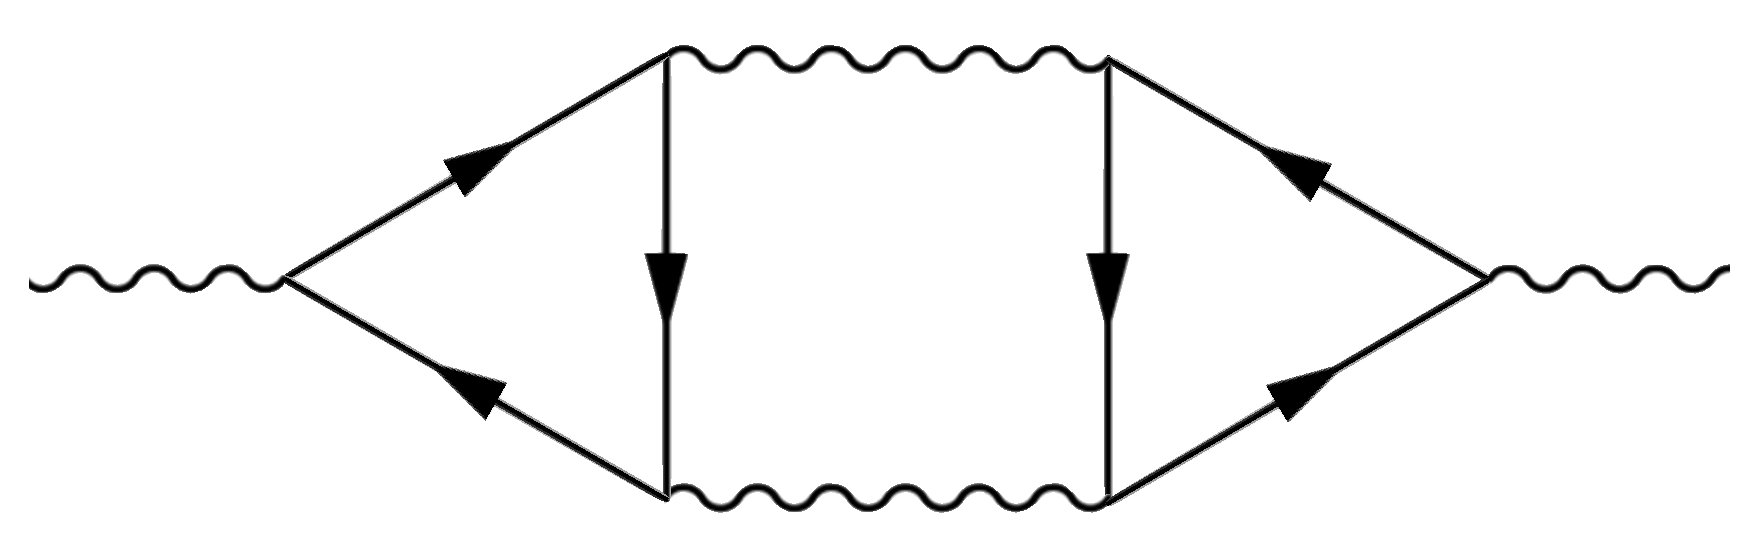
\includegraphics[scale=.25]{imgs/gauge_anomaly}
	\end{center}
\caption{\small ゲージボソンの質量に寄与するFeynman図。} \label{anomalous gauge boson mass}
\end{figure}

自然性の議論を用いれば、ゲージボソン質量の下限まで導くことができる。ツリーレベルでは質量ゼロのゲージボソンから出発し、第$N$クォークが三角形ループ内を伝播する、図\ref{anomalous gauge boson mass}に示したFeynman図を考えよう。アノマリーに詳しい読者なら、このグラフが、カイラルアノマリーの特徴である三角形フェルミオン図二つを、二本の光子線で貼り合わせたものであることに気づくだろう。この3ループ図にはUV発散があるが、ゲージ不変性を保つように正則化する方法はない。この図を低エネルギーEFTでマッチングするには、他の項に加えて、次の質量をもつゲージボソンの質量項を加える必要がある。
%
\begin{align} \label{m_A}
	m_A^2 \sim \left[\frac{1}{(4 \pi)^2}\right]^3 \times (e q_N)^6 \times (2 y v)^2 . 
\end{align}
%
右辺の三つの因子の起源は明らかだろう。各ループに対して一つのループ因子$1/(4 \pi)^2$、各頂点に対して一つの因子$e q_N$があり、ツリーレベルではゲージボソン質量をゼロと仮定したため、フェルミオン質量$2 y v$が、この図に現れる唯一の質量スケールである。また、式\eqref{m_A}は、純粋に低エネルギーEFTの文脈で定義される量を用いて、次のように書き換えられる。
%
\begin{align} \label{m_A 2}
	m_A^2 \sim \left(\frac{e}{4 \pi}\right)^6 \times \left(\sum_{j=1}^{N-1} q_j^3 \right)^2 \times \Lambda^2 ,
\end{align}
% 
ここで$\Lambda$はEFTの強結合スケールである。\emph{後から振り返れば}、実際には次の考察に基づいて、この結果を推測することもできた。
%
\begin{enumerate}
	\item EFTの強結合スケールが、この問題の唯一のスケールである。
	\item Lagrangianは$e \to -e, A_\mu \to - A_\mu$のもとで不変であるため、物理量は$e$の二乗にしか依存しえない。
	\item アノマリー係数は、$U(1)$が実際に対称性であるかどうかを制御する量であるため、質量がこの係数に比例するのは理にかなっている。
	\item Lagrangianは$e \to -e, q_j \to - q_j$のもとで不変であるため、$e$の各因子には$q_j$の因子が伴うはずである。
\end{enumerate}
%
式\eqref{m_A 2}の表式は、実際には非常に一般的であり、自然性に基づいて、アノマリーをもつフェルミオンの組み合わせを含むEFTにおける、Abelianゲージ場の質量の下限を与える。



\subsectionlink{さらに学ぶための文献}

カイラル摂動論に関する、より詳しい総説として、文献~\cite{Ecker:1994gg,Pich:1995bw,Scherer:2002tk}がある。Goldstoneモードの一般的なEFTについては、総説~\cite{Burgess:1998ku,Pich:2018ltt}が重点的に扱っている。アノマリーについては文献~\cite{Harvey:2005it,Bilal:2008qx}、アノマリーをもつYang-Mills理論については文献\cite{Preskill:1990fr}で、さらに詳しく学ぶことができる。




\newpage



\sectionlink{非相対論的フェルミオンのEFT}


\subsectionlink{真空中の非相対論的フェルミオン} \label{sec: NR fermions in vacuum}

\ref{sec: toy model}節のトイモデルでは、フェルミオンが相対論的、すなわちエネルギーが$E \gg m c^2$であったため、パワーカウンティングは特に容易であった。\footnote{この節では、$c$の因子をすべて復活させる。特に、$\d_0 = \d_t / c$である。}その結果、$\Psi$に作用する偏微分の各成分はすべて同じように、すなわち$\d_\mu \sim E /c$とスケールした。しかし、運動量が$p \ll mc$である非相対論的フェルミオンの散乱過程では、もはやこれは成り立たない。この場合は
%
\begin{align}
	\d_\mu \Psi \sim i \, (- m c, \, \vec p \, ) \, \Psi,
\end{align}
%
であり、第0成分は空間成分よりもはるかに大きくなる。明確にしておくと、微分によってスケーリングが異なること自体が必ずしも問題なのではない。後に見るように、これは多くのEFTで起こる。ここでの問題は、第0成分がフェルミオンの運動量、あるいは同じことだがエネルギーに応じてまったくスケールしないことである。このため、$\Psi$の高階時間微分は低エネルギーで必ずしもより強く抑制されず、したがってLagrangianの演算子は運動量のべきに従って明確には整理されない。幸い、次の\high{位相の再定義}によって新しい場$\tilde \Psi$を導入すれば、この問題は容易に解決できる。
%
\begin{align} \label{Psi tilde def vacuum}
	\Psi (t, \vec x)  \equiv e^{- i m c^2 t} \tilde \Psi (t, \vec x) 
\end{align}
%
すると、$\tilde \Psi$の微分は
%
\begin{align} \label{Psi tilde derivatives}
	\d_\mu  \tilde \Psi = \d_\mu \left( e^{i m c^2 t} \Psi \right) \sim i \, (- \frac{p^2}{2mc}, \, \vec p \, ) \, \tilde \Psi
\end{align}
%
とスケールする。したがって、微分を余分に含む演算子は、運動量が有効理論の強結合スケールに比べて小さいとき、より強く抑制される。

この場の再定義をLagrangianの段階で直接実行してみることは有益である。例えば、式\eqref{4pt tree effective theory}の作用で$(\bar  \Psi \gamma^5 \Psi)^2 \to (\bar  \Psi  \Psi)^2$としたものを考えよう。$c$のべきとガンマ行列をすべて明示すれば、作用を$\tilde \Psi$によって直接、次のように書ける。
%
\begin{align} \label{4pt tree effective action with c}
	S_{\rm eff} = \int dt \, d^3 x \, c \left\{ \tilde \Psi^\dag \l[ \frac{ i \d_t}{c}  +  i \gamma^0 \gamma^i \d_i +  (1 - \gamma^0) m c  \r] \tilde \Psi - \frac{y^2}{2 M^2c} (\tilde \Psi^\dag \gamma^0 \tilde \Psi )^2\right\} \ .
\end{align}
%
4次相互作用の前の$1/c$という因子は、結合定数を再定義すれば常に吸収できるが、後の便宜のために導入してある。$\tilde \Psi$の微分に対するパワーカウンティング則\eqref{Psi tilde derivatives}によれば、角括弧内の支配的な項は$m c$に比例する項である。このことから、射影行列\footnote{$P_\pm$が実際に射影演算子の定義を満たすこと（$P_\pm^2 = P_\pm$）は容易に確かめられる。さらに、これらは互いに直交し（$P_+ P_- = P_- P_+ = 0$）、完全系をなす（$P_+ + P_- = 1$）。}$P_\pm \equiv \tfrac{1}{2} (1 \pm \gamma^0)$を導入して、$\tilde \Psi$を$\tilde \Psi_\pm \equiv P_\pm \tilde \Psi$の和に分解するのが自然である。Lagrangianの主要な2次項は$mc^2  \tilde \Psi_+^\dag \tilde \Psi_+$なので、この非相対論的EFTの展開パラメータである$p/mc$について摂動的に計算することにより、$\tilde \Psi_+$を積分消去し、$\tilde \Psi_-$だけの有効Lagrangianを得ることができる。非相対論的粒子では$p = m v$なので、この展開パラメータは$v /c$とも表せることに注意しよう。
%
\begin{eBox}
%
{\bf 演習4.1：}$\tilde \Psi_+$をツリーレベルで積分消去し、$p/mc$の最低次で$\tilde \Psi_-$の有効作用を導け。
%
\end{eBox}

物理的には、非相対論的領域でモードの半分を積分消去できるのは、例えば粒子だけが関与する低エネルギー散乱では、エネルギー保存により反粒子を生成できないからである。$\gamma^0$が対角的となるDirac行列のDirac表示~\cite{Zee:2003mt}を用いれば、このことをより明示的に示せる。\footnote{非相対論的極限では、この基底は文献~\cite{Srednicki:2007ab}で用いられている、$\gamma^5$が対角的となるWeyl基底よりも便利である。二つの基底におけるスピノルは、$S = \frac{1}{\sqrt{2}} \left( \begin{smallmatrix} 1 & 1 \\ -1 & 1 \end{smallmatrix} \right)$とした線形変換$\Psi_{\rm Dirac} = S \, \Psi_{\rm Weyl}$によって結び付いている。}
%
\begin{align} \label{2-spinor def}
	\gamma^0 = \begin{pmatrix}
		1 &  0 \\ 0 & -1 
	\end{pmatrix} \qquad \Longrightarrow \qquad \tilde \Psi_- = \begin{pmatrix}
		0 \\ \psi 
	\end{pmatrix} .
\end{align}
% 
このとき、2成分スピノル$\psi$に対する最低次のLagrangianは、次で与えられる。
%
\be \label{S psi}
S_{\rm eff} = \int dt \, d^3 x \left\{ \psi^\dag \l( i \d_t  + \frac{\nabla^2}{2 m} \r) \psi  - \frac{y^2}{2 M^2} (\psi^\dag \psi )^2 \right\} . 
\ee
%

ここで、さらにパワーカウンティングを行おう。式\eqref{Psi tilde derivatives}の微分のスケーリングから、$d t d^3 x \sim 1/p^5$と分かる。前の二つの節で論じた例とは異なり、運動量に関するスケーリングは、もはや自然単位系の次元解析からは推論できないことに注意しよう。$\psi$のスケーリングは、通常どおり自由作用がスケールしないという要請によって定まり、$\psi \sim p^{3/2}$となる。したがって、残しておいた4次相互作用は$\sim p$とスケールし、運動量が小さいときには非関連であることが分かる。\footnote{式\eqref{expectation values}と、$\slashed{\partial} \, u_j \to i \d_t  + \frac{\nabla^2}{2 m}$とした非相対論的なLSZ公式を用いれば、このスケーリングが、摂動論の最低次では4点振幅が定数となることと整合することを確かめられる。}実際、真空中のフェルミオンだけが関与する\emph{あらゆる}相互作用は非関連であることが分かる。有限密度のフェルミオンでは事情が異なることを、この後すぐに見る。その前に、有効作用\eqref{S psi}の対称性が、出発点とした相対論的作用の対称性とどのように関係するかを論じよう。



\subsectionlink{縮約された対称性と偶発的対称性}


相対論的Lagrangianは、$\Psi$がDirac表示で次のように変換するならば、Lorentz変換$x^{\mu \, \prime} = \Lambda^\mu{}_\nu x^\nu$の下で不変である。
%
\begin{align} \label{trans rule relativistic spinor}
	\Psi' (x') = 
		\frac{1}{2}\begin{pmatrix}
		 e^{\frac{i}{2} \vec \sigma \cdot (\vec \alpha + i \vec \beta)} + e^{\frac{i}{2} \vec \sigma \cdot (\vec \alpha - i \vec \beta)} & e^{\frac{i}{2} \vec \sigma \cdot (\vec \alpha + i \vec \beta)} - e^{\frac{i}{2} \vec \sigma \cdot (\vec \alpha - i \vec \beta)} \\ e^{\frac{i}{2} \vec \sigma \cdot (\vec \alpha + i \vec \beta)} - e^{\frac{i}{2} \vec \sigma \cdot (\vec \alpha - i \vec \beta)} & e^{\frac{i}{2} \vec \sigma \cdot (\vec \alpha + i \vec \beta)} + e^{\frac{i}{2} \vec \sigma \cdot (\vec \alpha - i \vec \beta)}
		\end{pmatrix} \Psi (x) ,
\end{align}
%
ここで、$\alpha$は回転を、ベクトル$\vec \beta \equiv \vec v / c$はLorentzブーストをパラメータ化する。$p/mc$展開の最低次では、式\eqref{trans rule relativistic spinor}から、2成分スピノル$\psi$の変換則として次を得る。
%
\begin{align}
	\psi (t, \vec x^{\, \prime}) = e^{i m (v^2 t/2 - \vec v \cdot \vec x)} e^{i \vec \sigma \cdot \vec \alpha/2} \psi (t, \vec x) ,
\end{align}
% 
一方、座標は回転およびGalileiブーストの下で通常どおり変換する。
%
\begin{eBox}
%
{\bf 演習4.2：}微分演算子$D \equiv i \d_t  + \nabla^2/(2 m)$が、$\vec x^{\, \prime} = \vec x - \vec v \, t$に対して$D' \psi' (t, \vec x^{\, \prime}) = e^{i m (v^2 t/2 - \vec v \cdot \vec x)} D \psi (t, \vec x)$となるという意味で、ブーストに関する共変微分であることを示せ。
%
\end{eBox}
%

この結果を用いれば、非相対論的Lagrangian\eqref{S psi}が回転とGalileiブーストの両方の下で不変であることが直ちに分かる。もちろん、これはLorentz不変性の$c \to \infty$極限にほかならない。より適切な用語がないので、これを\high{縮約された対称性}と呼ぶことにする。Galilei変換の代数は、Lorentz代数の縮約から得られるからである~\cite{Weinberg:1995mt}。

また、座標を変えずに$\psi$に作用する内部$U(2) = SU(2) \times U(1)$対称変換も存在する。$U(1)$部分群は相対論的作用の$U(1)$対称性の名残である。ただし、低エネルギーでは、運動学によって保存されるのは粒子数と反粒子数の差ではなく、粒子数そのものである。一方、$SU(2)$部分群には相対論的な対応物がなく、非相対論的理論ではスピンと座標を独立に回転させられるという、よく知られた事実を表している。

この付加的な$SU(2)$は、\high{偶発的対称性}の好例である。名前のとおり、これはEFTの粒子の構成と基本的な対称性が十分に強い制約を課し、EFT展開のある次数までは、その対称性の下で不変な演算子しか書けないために、偶然生じる対称性である。偶発的対称性は、最終的にはEFTの高次補正によって破れる。したがって、十分な精度でEFTを検証すれば、原理的には偶発的対称性と基本的対称性を区別できる。標準模型における偶発的対称性の例には、バリオン数およびレプトン数の保存に対応する対称性や、Higgsセクターのカストディアル対称性がある。

最低次の有効作用\eqref{S psi}を振り返ると、対称性の議論だけから、その形を\emph{ほぼ}推測できたことが分かる。空間回転に対する不変性は、各$\psi$のスピン添字を$\psi^\dag$のもつ添字と縮約することを要求し、Galileiブーストに対する不変性は、共変微分$D$を用いることを要求する。確かに、微分の1次では$(D \psi)^\dag \psi$という形の項も加えられるが、部分積分を除けば、これは$\psi^\dag D \psi$と等価であることが容易に示せる。むしろ不思議なのは、2次項$\psi^\dag \psi$が存在しないことである。この項は、これまで論じたすべての対称性と両立し、しかも、この項が存在しないからといって対称性が増大するわけではない。これまでの自然さに関する議論に照らすと、有効作用\eqref{S psi}は微調整されているのではないかと心配になるかもしれない。実際には、このような項は繰り込まれないことが容易に分かるので、ゼロに設定することは自己無撞着である。

例えば、相対論的スカラーの質量項を繰り込むであろう次のループ補正を考えよう。\\

%
\begin{align}
	\parbox[t][10mm][b]{20mm}{\begin{fmfgraph*}(50,60) 
	\fmfleft{i} \fmfright{o} 
	\fmf{fermion}{i,v,o} 
	\fmffreeze
	\fmf{fermion,tension=.5}{v,v}
	\end{fmfgraph*}} = - i \frac{y^2}{M^2} \int \frac{dE d^3 p}{(2 \pi)^3} \frac{i}{E -p^2/2m + i \epsilon} = - i \frac{y^2}{M^2} \int \frac{d Q^2 d^3 p}{(2 \pi)^3} \frac{i}{Q^2 -p^2 + i \epsilon } . 
\end{align}
%
この積分はUV発散するが、積分変数$E$を再定義すると長さのスケールを何も含まなくなるので、次元正則化ではゼロになる。同様の議論は、2点関数に対する高次のループ補正にも当てはまる。$2m$の因子をエネルギーに吸収した後には、ループ積分中のスケールは外部のエネルギーと運動量だけとなる。これは、次元正則化では、ループが微分を含む2次演算子だけを繰り込むことを意味する。

演算子$\psi^\dag \psi$が繰り込まれないことには、直観的な説明がある。標準的な議論によって作用\eqref{S psi}から$U(1)$のNoetherカレントを計算すると、演算子$\psi^\dag \psi$が$U(1)$電荷の密度であることが分かる。したがって、$\Delta L = \mu_{\rm nr} \psi^\dag \psi$という形の項を加えることは、電荷密度に対するソース、すなわち化学ポテンシャルを導入することに対応する。これは、実験者がループ補正を気にせず、自由に行えるはずの操作なのである。



\subsectionlink{有限密度における非相対論的フェルミオン}


 
次に、フェルミオンが有限密度で存在する状態を考えよう。これは、有限の化学ポテンシャル$\mu_{\rm nr} \ll m c^2$を導入し、問題に新たなスケールを加えることで実現できる。温度がゼロのとき、エネルギーがFermiエネルギー$E_F \equiv \mu_{\rm nr}$以下の状態はすべて占有され、それ以外の状態はすべて空である。この条件は、占有された運動量状態と占有されていない運動量状態を隔てる、運動量空間内の閉じた面、すなわち\emph{Fermi面}を定める。自由フェルミオンの場合、これは半径$p_F = \sqrt{2 m E_F}$の球面にすぎない。相互作用があるとこの球面は変形し、Fermi面はより複雑な形状をとりうる。

\high{Fermi液体}の理論は、温度ゼロ・有限密度における重要な集団励起が、依然としてフェルミオンであるという仮定に基づいている。弱結合領域では、これらの励起を、相互作用によって「衣をまとい」、\footnote{ここで意味しているのは、相互作用によってFermi面近傍の1粒子状態の分散関係が変化するということである。}Fermi面のわずか上に励起されたフェルミオンと考えられるので、この仮定は直観的に理解できる。しかし驚くべきことに、この仮定は多くの強結合系においても、経験的に正しいことが分かっている。これらのフェルミオン的励起は、系を構成する実際のフェルミオンと区別するために、しばしば準粒子と呼ばれる。

フェルミオン的準粒子だけが唯一の可能性ではないことを指摘しておこう。例えば、低温のヘリウム3や通常の超伝導体で起こるように、フェルミオンが対を作ってボソンとなり、それが低エネルギーで凝縮する場合もある。この可能性については、この節の終わりに簡単に論じる。フェルミオンの強結合系の中には、準粒子励起そのものがまったく存在しないものさえあり、そのような系は単に\emph{非Fermi液体}と呼ばれる。以下ではFermi液体に対象を絞り、そのフェルミオン的準粒子を記述するEFTを導く。

Fermi面のわずか上に励起された準粒子は、エネルギーが$E_F$からわずかにずれたフェルミオンである。これは、エネルギーが$m c^2$からわずかにずれた非相対論的フェルミオンに関する先ほどの議論を思い起こさせるはずである。ここでの違いは、Fermi面上の粒子が有限の運動量${\vec p}_F$ももつことである。これを扱うため、\ref{sec: NR fermions in vacuum}節の手順を一般化し、非相対論的フェルミオン場$\psi$を次のようにパラメータ化する。
%
\begin{align} \label{Psi tilde def}
	\psi (t, \vec x) \equiv e^{- i E_{F} t} \sum_{{\vec p}_F} e^{i {\vec p}_F \cdot \vec x} \, \psi_{{\vec p}_F} (t, \vec x) .
\end{align}
%
このように、$E_F$だけでなく$\vec p_F$にも依存する位相を取り出すことによって、単一の場$\psi$を、Fermi面上の可能なすべての運動量でラベル付けされた場$\psi_{{\vec p}_F}$の集まりに、実質的に置き換えた。構成から、これらの場は、$\epsilon \ll E_F$として$\d_t \psi_{{\vec p}_F} \sim \epsilon \,\psi_{{\vec p}_F}$を満たす励起を記述する。したがって、このEFTの自然な展開パラメータは、比$\epsilon / E_F$である。

次に、$\psi_{{\vec p}_F}$の有効作用を書き下す作業に移ろう。強く相互作用する系では、例えば\ref{sec: NR fermions in vacuum}節の非相対論的モデルで行ったように、基礎となる理論からEFTを直接導出することはできない。このため、代わりに対称性を指針として用いる。$\psi$の変換性から出発すれば、場$\psi_{{\vec p}_F}$が時空対称性の下で次のように変換しなければならないことは容易に示せる。
%
\begin{subequations} \label{sp symmetries psi p_F}
\begin{align}
\text{時間並進：} \qquad \psi_{{\vec p}_F}' (t + c, \vec x) &= e^{i E_F c} \,\psi_{{\vec p}_F} (t, \vec x) \\
\text{空間並進：} \qquad \psi_{{\vec p}_F}' (t, \vec x + \vec c) &= e^{-i \vec p_F \cdot \vec c} \,\psi_{{\vec p}_F} (t, \vec x) \\
\text{空間回転：} \qquad  \psi_{R \cdot {\vec p}_F}' (t, R \cdot \vec x ) &= M(R) \,\psi_{{\vec p}_F} (t, \vec x) \\
\text{Galileiブースト：} \qquad  \psi_{{\vec p}_F- m \vec v}' (t, \vec x - \vec v t) &= \psi_{{\vec p}_F} (t, \vec x) , \label{boost transf rule}
\end{align}
\end{subequations}
%
ここで、$M(R)$は回転$R$のスピン$1/2$表現である。
%
\begin{eBox}
%
{\bf 演習4.4：}Galilei群の代数、特に交換関係
%
\begin{align}
	[ H, K_j ] = i P_j, \qquad \qquad [P_i, K_j ] = i M \delta_{ij} , \qquad \qquad [M, K_j ] = 0, 
\end{align}
を用いて、$\vec x^{\, \prime} = \vec x - \vec v \, t$となるブースト変換の下で、Fermi運動量とFermiエネルギーが次のように変化することを示せ。
%
\begin{align} 
	\vec p_F^{\, \prime} = \vec p_F - m \, \vec v, \qquad \quad E_F' = E_F - \vec p_F \cdot \vec v + \frac{m v^2}{2}. \label{pF EF transformation rules}
\end{align}
%
次に、これらの結果を用いて変換則\eqref{boost transf rule}を導け。最後に、Galileiブーストは運動量空間内のFermi面の位置を変えるが、その形は変えないことを確かめよ。
%
\end{eBox}
%
相対論的補正を無視できる範囲では、スピン回転に関する偶発的対称性も課すべきである。
%
\begin{align} \label{int symmetry psi p_F}
\text{スピン回転：} \qquad \psi_{{\vec p}_F}' (t, \vec x) &= U \,\psi_{{\vec p}_F} (t, \vec x) .
\end{align}
%

上の対称性のうち、最終的にどれを課すかは、考えている物理系による。例えば、金属中の電子では、背景の格子がブーストと回転を自発的に破る。これらの対称性はフォノンによって非線形に実現されているが、フォノンとの結合を考慮しなければ、陽に破れているように見える。以下では、可能な限り単純な状況、すなわちフェルミオンのみが存在し、背景の格子がない場合を考える。この場合、有効作用はこれまで論じたすべての変換の下で不変でなければならず、Fermi面は球面のままである。

変換則\eqref{sp symmetries psi p_F}と\eqref{int symmetry psi p_F}をすべて合わせると、有効作用の形に強い制約が課される。特に、時間並進不変性から、各$\psi_{{\vec p}_F}$は$\psi_{{\vec p}_F^{\, \prime}}^\dag$と対になって現れなければならない。一方、空間並進は、すべての$\psi_{{\vec p}_F}$のラベルの総和から、すべての$\psi_{{\vec p}_F}^\dag$のラベルの総和を引いたものがゼロになることを要求する。最後に、すべてのスピノル添字が縮約されていれば、スピン回転に対する不変性が保証される。

ブーストの下での$\psi_{\vec p_F}$の変換性により、ブーストに対して不変な共変微分を導入する必要がある。そのためには、Fermi面の各点で法線ベクトル
%
\begin{align}
	\vec v_F \equiv \frac{\d E_F}{\d \vec p_F},
\end{align}
%
を定義すると便利である。これは通常、\emph{Fermi速度}と呼ばれる。このベクトルがブーストの下で予想どおり$\vec v_F^{\, \prime} = \vec v_F - \vec v$とシフトし、その結果、微分演算子$\mathcal D \equiv \d_t + \vec v_F \cdot \vec \nabla$が不変になることは容易に分かる。微分の最低次では、すべての対称性を保ったまま書き下せる運動項は一つしかなく、次で与えられる。
%
\begin{align} \label{S kin fermi liquids}
	S_{\rm kin} = \sum_{\vec p_F} \int dt \, d^3 x \, \psi_{\vec p_F}^\dag i \mathcal D \, \psi_{\vec p_F} \ , 
\end{align}
%
ここでは、スピノル添字は縮約されているものとする。

\begin{figure}
	\begin{center}
		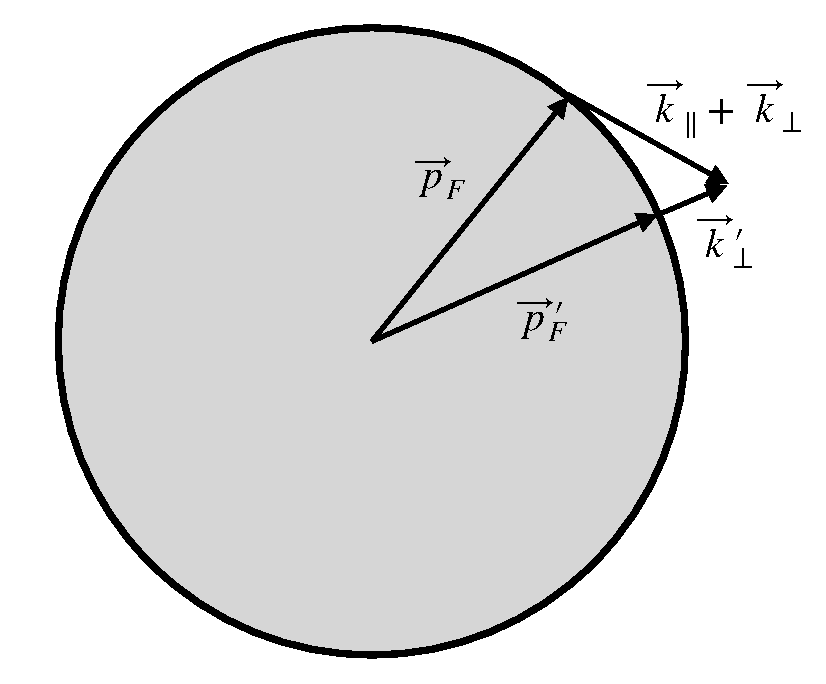
\includegraphics[scale=0.4]{imgs/fermi_surface_sphere}
	\end{center}
	\vspace{-.6cm}
\caption{\small Fermi面に平行な運動量と垂直な運動量。} \label{fig: Fermi surface}
\end{figure}

主要な運動項を決定したので、このEFTのパワーカウンティング則を導ける。まず、不変な微分演算子が一様にスケールするためには、次が必要である。
%
\begin{align} \label{fermi liquids power counting rule 1}
	\vec v_F \cdot \vec \nabla \sim \d_t \sim \epsilon.
\end{align}
%
運動項が決定するのは、空間勾配の一成分、すなわちFermi面に垂直な成分のスケーリングだけである。これは、これまでに考えた他のすべてのモデルとは異なる。その理由を理解するため、各Fourierモード$\psi_{{\vec p}_F} (t , \vec k)$の運動量$\vec k$を、$\vec p_F$におけるFermi面に平行な方向と垂直な方向に分解しよう。
%
\begin{align}
	\vec k = \hat v_F (\hat v_F \cdot \vec k ) + \hat v_F \times ( \vec k \times \hat v_F) \equiv \vec k_\perp + \vec k_\parallel \ .
\end{align}
%
すると、図\ref{fig: Fermi surface}に示すように、場のラベルを再定義することで、Fermi面に平行な運動量成分は常に吸収できる。より正確には、Fermi球面上の異なる点における場のFourierモードの間には、次の関係が成り立つ。
%
\begin{align}
	\psi_{\vec p_F} (t, \vec k_\parallel + \vec k_\perp) = \psi_{\vec p_F^{\, \prime}} (t, \vec k_\perp^{\, \prime}), 
\end{align}
%
ただし、各量は次のように与えられる。
%
%
\begin{align}
	k_\perp' = | \vec p_F + \vec k_\parallel + \vec k_\perp|, \qquad \qquad \hat k_\perp' = \hat p_F' = \frac{\vec p_F + \vec k_\parallel + \vec k_\perp}{| \vec p_F + \vec k_\parallel + \vec k_\perp|} \ .
\end{align}
%
したがって、場$\psi_{\vec p_F}$はFermi面に垂直な方向の運動量だけをもつと常に仮定できる。よって、積分測度と場は
%
\begin{align} \label{fermi liquids power counting rule 2}
	dt\,  d^3 x \sim d t \, d x_\perp d^2 x_\parallel \sim \epsilon^{-2}, \qquad \qquad \psi_{\vec p_F} \sim \epsilon^{1/2}, 
\end{align}
%
とスケールしなければならない。これによって、運動項\eqref{S kin fermi liquids}が微分展開において$\mathcal{O}(1)$であることが保証される。

パワーカウンティング則\eqref{fermi liquids power counting rule 1}と\eqref{fermi liquids power counting rule 2}が得られたので、準粒子間の相互作用を論じることができる。まず、原理的には、書き下せる関連な2次項が一つあることに注意しよう。それは
%
\begin{align} \label{quadratic int fermi liquids}
	-  \sum_{\vec p_F} \int dt \, d^3 x \, \Delta \, \psi_{\vec p_F}^\dag  \psi_{\vec p_F} \sim \epsilon^{-1} , 
\end{align}
% 
である。ここで、$\Delta$は、ブースト不変性を保つために$\vec p_F$に依存してはならないパラメータである。この項はエネルギーギャップを加えることによって、準粒子の分散関係を$\epsilon \to \vec v_F \cdot \vec k + \Delta$と変更する。言い換えると、この演算子はすべての準粒子のエネルギーを一定量だけシフトさせる。このようなシフトは常にFermi面の再定義に吸収できる。そのため、2次演算子\eqref{quadratic int fermi liquids}は、場の位相を$\psi_{\vec p_F}' \equiv e^{i \Delta t} \psi_{\vec p_F}$と再定義することによって、常に取り除ける。

さらに興味深いのは、模式的に次の形をもつ4次の周辺的相互作用が存在することである。
%
\begin{align} \label{fermi liquids marginal interactions}
	S_{\rm int} = \sum_{\vec p_{F, i}}{\vphantom{\sum}}' \int dt \, d^3 x \,  g \,  \psi_{- \vec p_{F,3}}^\dag   \psi_{\vec p_{F,1}}  \, \psi_{- \vec p_{F,4}}^\dag \psi_{\vec p_{F,2}} \sim 1 \ ,
\end{align}
%
ここで、総和のプライムは、並進不変性が課す制約$\vec p_{F,1} +   \vec p_{F,2} + \vec p_{F,3} +\vec p_{F,4} = 0$を表している。さらに、係数$g$は、すべてのスピノル添字が$SU(2)$不変な形で縮約されるような添字構造をもち、回転不変性およびブースト不変性と両立する最も一般的な仕方で、ラベル$\vec p_{F, i}$に依存してよい。
%
\begin{figure}[t]
	\begin{center}
		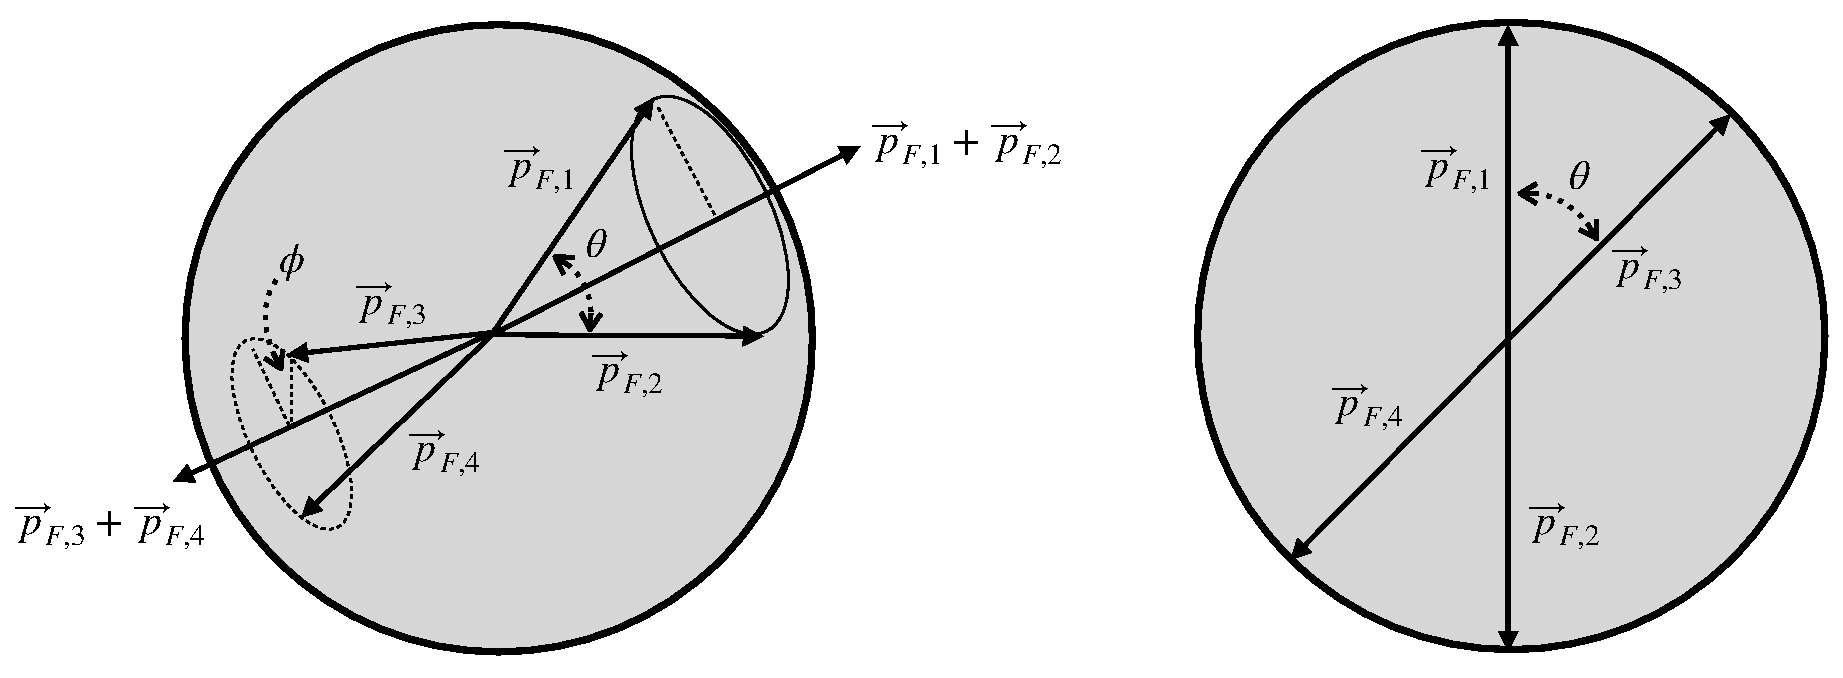
\includegraphics[scale=0.4]{imgs/scattering}
	\end{center}
	\vspace{-.6cm}
\caption{\small Fermi面上で運動量を保存する相互作用。} \label{fig: scattering Fermi surface}
\end{figure}
%

まず、運動量依存性を論じよう。すべての$\vec p_{F,i}$が同時にFermi面上になければならないので、並進不変性の要請は特に厳しい制約となる。これを見るために、運動量空間の任意の二方向に沿って$\vec p_{F,1}$と$\vec p_{F,2}$を選ぼう。この二つのベクトルは、図\ref{fig: scattering Fermi surface}の右図に示すように、$\vec p_{F,1} + \vec p_{F,2}$の方向を軸とする円錐上にある。運動量保存は、$\vec p_{F,3}$と$\vec p_{F,4}$が、同じ軸をもち、原点に対して反対向きの円錐上にあることを要求する。全体の回転を除けば、この配置は二つの角度、すなわち$\vec p_{F,1}$と$\vec p_{F,2}$の間の角度$\theta$、および$\vec p_{F,1}, \vec p_{F,2}$の張る平面と$\vec p_{F,3}, \vec p_{F,4}$の張る平面の間の角度$\phi$だけで完全に記述される。文献~\cite{Shankar:1993pf}に従い、この運動量配置を\emph{零音波チャネル}と呼ぶ。

このチャネルは、$p_{F,1} = - \vec p_{F,2}$という特殊な場合には明確に定義できなくなる。このとき、運動量保存から$p_{F,3} = - \vec p_{F,4}$となる。これらの「背中合わせ」の相互作用は、図\ref{fig: scattering Fermi surface}の右図に示すように、一つの角度$\theta$で特徴付けられる。この種の相互作用を\emph{BCSチャネル}と呼ぶ。
%
\begin{eBox}
%
{\bf 演習4.5：}零音波チャネルの角度$(\theta,\phi)$とBCSチャネルの角度$\theta$を、ラベル$\vec p_{F,i}$を用いて表せ。
%
\end{eBox}
%
次に、BCSチャネルに対象を絞ろう。この場合、4次相互作用は次の形をとる。
%
\begin{align}
	S_{\rm BCS} = \sum_{\vec p,\vec p^{\, \prime}} \int dt \, d^3 x \,  g_{abcd} (\theta)  \psi_{\vec p^{\, \prime}}^{a \dag}   \psi_{\vec p}^b  \, \psi_{- \vec p^{\, \prime}}^{c\dag} \psi_{- \vec p}^d \ ,
\end{align}
%
ここで、$\theta$は$\vec p$と$\vec p^{\, \prime}$の間の角度である。$SU(2)$スピン対称性が許す独立な添字構造は二つだけであり、次のように書けることは容易に確かめられる。
%
\begin{align} \label{BCS channel tensor structure}
	g^{abcd} (\theta) &= g_1 (\theta) \, \delta^{ab} \delta^{cd} + g_2	 (\theta) \, \vec \sigma^{ab} \cdot \vec \sigma^{cd} \ . 
\end{align}
%
関数$g_i(\theta)$はさらにLegendre多項式に分解でき、これによって無限個の結合定数$g_{i, \ell}$が実質的に導入される。
%
\begin{align}
	g_i (\theta) = \sum_{\ell} g_{i,\ell} P_\ell (\cos \theta) \ .
\end{align}
%
一見すると、これは、展開パラメータの任意の固定次数において作用に現れる結合定数は有限個であるべきだという、EFTに関する標準的な通念に反するように見える。これは、その通念が、EFTに含まれる場の数は有限であるという暗黙の仮定に基づいているためである。今回の場合、$\psi$を無限個の場$\psi_{\vec p}$に実質的に置き換えている。しかし、予言能力は失われないことに注意しよう。$\theta$の値を固定すると、結合$g_i (\theta)$は、「ソフト」な運動量$\vec k$の運動学的配置が任意である過程を記述する。

% 
\begin{eBox}
%
{\bf 演習4.6：}演習4.5で導いた結果を用いて、零音波チャネルの角度がパリティ変換の下で$(\theta, \phi) \to (\theta, \pi+ \phi)$と変換することを示せ。次に、理論がパリティ不変ならば、零音波チャネルで可能なテンソル構造も式\eqref{BCS channel tensor structure}の形に限られることを示せ。
%
\end{eBox}
%

以上から、フェルミオンが有限密度で存在すると、真空の場合に比べてパワーカウンティング則が大きく変わり、式\eqref{fermi liquids marginal interactions}の形の周辺的相互作用が存在できることが分かった。これらの相互作用は零音波とBCSという二つのチャネルに分けられ、原理的には無限個の結合で記述される。通常どおり、量子補正により、結合の異常次元に応じて、これらの相互作用は関連にも非関連にもなりうる。引力的な相互作用は関連となり、斥力的な相互作用は非関連となることが分かっている~\cite{Shankar:1993pf}。

ある系において結合が正か負かは、実験を行うか、基礎となるUV理論にマッチングすることによってしか決定できない。そのUV理論の結合は、別の実験によって決定されていなければならない。しかし、一般論として、関連となる結合は低エネルギーで顕著な現象を生み出すと期待できる。例えば、ヘリウム3では$\ell =1$のBCSチャネルの結合が周辺的に関連であり、そのためヘリウム原子が対を作って低温で凝縮し、超流動が生じる。一方、金属では$\ell =0$のBCSチャネルが関連となり、通常の超伝導を引き起こす。これらの現象を詳しく論じることは本講義の範囲を大きく超えるが、関心のある読者のために、この節の最後に有用な資料をいくつか挙げてある。全体を通じて、Fermi液体論も他のEFTと同じく、自由度、展開パラメータ、対称性の特定の選択に基づいていることが伝われば幸いである。このわずかな仮定だけから、数多くの興味深い物理が導かれる。




\subsectionlink{非相対論的QED}


次に、少し複雑な例である非相対論的QED（NRQED）を考える。これは、真空中の非相対論的フェルミオンが、式\eqref{S psi}の接触相互作用ではなく、長距離の電磁相互作用を受けるEFTである。これまでに論じたEFTとは異なり、NRQEDには考慮すべき運動学的領域が複数あり、その結果、パワーカウンティングはかなり複雑になる。例えば、NRQEDを用いて、等しい質量の構成粒子からなる束縛状態を研究し、速度$v$のべきによる系統的な展開で観測量を計算できる。\footnote{この節では、再び$c=1$の単位系を用いる。}実際、ビリアル定理と不確定性原理を組み合わせれば、束縛状態では$v$が小さくなければならないことは容易に分かる。
%
\begin{align}
	\frac{m v^2}{2} \sim \frac{\alpha}{r} \lesssim \alpha \, m v \qquad \Longrightarrow \qquad v \lesssim \alpha \ll 1. 
\end{align}
% 
NRQEDの動機は、本講義でこれまでに扱った他のEFTの動機とは異なることを強調しておこう。ここでは、低エネルギーでは生成できないほど重い粒子を積分消去するわけでも、UVにおける強結合の物理や未知の物理の低エネルギーでの帰結をモデル化することが主目的でもない。むしろ、QEDのような十分に理解された摂動的理論を用いて、小さな速度$v$のべきによる展開として観測量を計算することに関心がある。これを最も効率的に実現するには、$v$に関するパワーカウンティングを作用の段階で直接実装できる、NRQEDのようなEFTへ移ればよい。

出発点は、通常のQEDの作用である。
%
\begin{align}
	S = \int d^4 x \left\{ \bar \Psi [i \gamma^\mu (\partial_\mu - i e A_\mu) - m ] \Psi - \frac{1}{4} F_{\mu\nu} F^{\mu\nu} - \frac{1}{2\xi} (\partial_\mu A^\mu)^2 \right\},
\end{align}
%
ここでは、ゲージ固定項をすでに明示的に加えてある。以下では、$\xi = 1$であるFeynmanゲージを用いる。$m$よりもはるかに小さいエネルギーでは、\ref{sec: NR fermions in vacuum}節で行ったのとまったく同じように、フェルミオン場の位相を再定義して反粒子を積分消去できる。$A^\mu = (\Phi, \vec A)$と書くと、次のツリーレベル有効作用を得る。
%
\begin{align} \label{NRQED action}
	S_{\rm eff}^{(0)} = \int dt \, d^3 x \left\{  \psi^\dag \left( i \partial_t  -e \Phi + \frac{\vec{D}^2}{2 m} + \frac{e}{2m} \vec B \cdot \vec \sigma \right) \psi  - \frac{1}{2} \partial_\mu A_\nu \partial^\mu A^\nu + \mathcal{O}(1/m^2) \right\} ,
\end{align}
%
ここで、2成分スピノル$\psi$は式\eqref{2-spinor def}で定義され、電場と磁場は通常どおりスカラーポテンシャルおよびベクトルポテンシャルから定義される~\cite{Jackson:1998nia}。また、$\vec D = \vec \nabla - i e \vec A$である。この作用は、式\eqref{S psi}の作用の接触相互作用を、光子を媒介とする相互作用に置き換えたものに相当する。
%
\begin{eBox}
%
{\bf 演習4.7：}式\eqref{NRQED action}のツリーレベル有効作用を導け。
\end{eBox}
%
$\vec B$に線形な項は、偶発的な$SU(2)$スピン対称性と空間回転を、それらの対角部分群にまで破ることに注意しよう。この項は$\vec \mu \cdot \vec B$という形をもち、$\vec \mu = 2 \mu_B \vec S$は磁気モーメントの密度、$\mu_B = q / (2 m c)$はBohr磁子、$\vec S = \frac{1}{2}\tilde \Psi_-^\dag \sigma^i \tilde \Psi_-$はスピン密度である。すなわち、これは、磁場中の磁気双極子密度のよく知られたポテンシャルエネルギーに負号を付けたものである。

\begin{figure}
	\begin{center}
		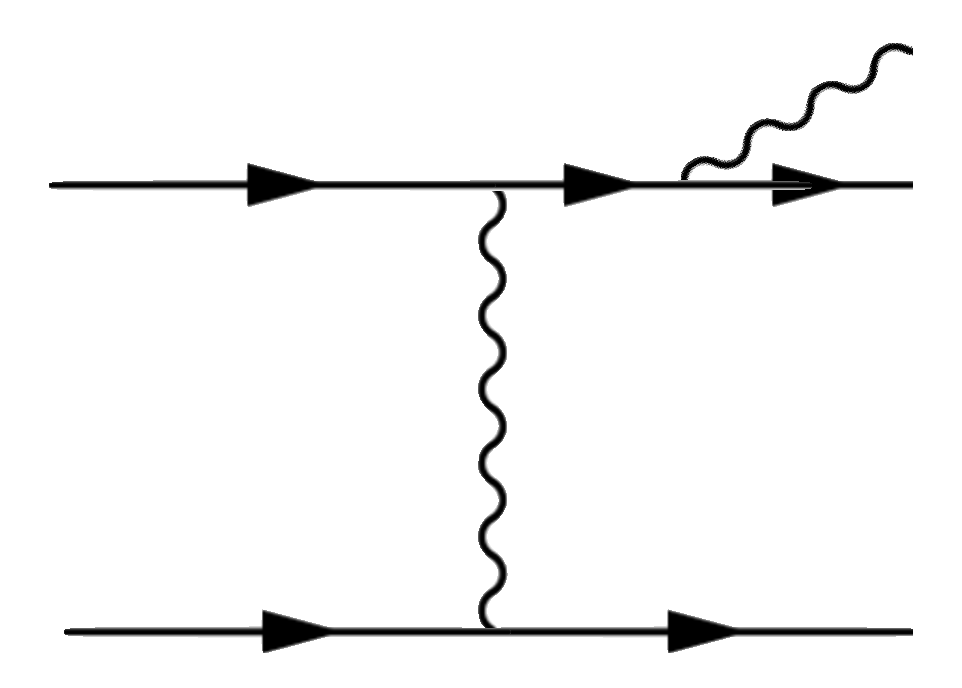
\includegraphics[scale=0.3]{imgs/NRQED}
	\end{center}
	\vspace{-.6cm}
\caption{\small QEDにおけるツリーレベル・ダイアグラムの例。} \label{fig:NRQED}
\end{figure}

ゲージ不変性は、作用\eqref{NRQED action}中の各微分がゲージポテンシャルとともに現れることを要求する。このため、有効作用を$m$の逆べきで展開することが、$p / m = v$のべきで展開することと等価であるかは、もはや明らかではない。等価となるためには、ポテンシャルも$v$のようにスケールする必要がある。これを確認するには、時間微分と空間微分がポテンシャルにどのように作用するかを知る必要がある。そうすれば、運動項が$\mathcal{O}(1)$の量であることを要求して、通常どおり場のスケーリング則を求められるからである。そのために、図\ref{fig:NRQED}のダイアグラムを考えよう。すべてのフェルミオン外線のエネルギーと運動量は$(mv^2, mv)$のオーダーである。したがって、散乱過程で交換され、光子内線によって運ばれるエネルギーと運動量も、一般には$(mv^2, mv)$のオーダーでなければならない。この運動学的領域を\emph{ポテンシャル}領域と呼ぶ。次に、この過程で放出される光子を考えよう。エネルギー保存により、そのエネルギーは高々$\mathcal{O}(mv^2)$である。対応する外線はオンシェルでなければならないので、そのエネルギーと運動量は$(mv^2, mv^2)$のオーダーでなければならない。この運動学的領域を\emph{ウルトラソフト}領域と呼ぶ。\footnote{これは\emph{放射}領域とも呼ばれる。}このことは、$A^\mu$が運ぶ運動量が、Feynmanダイアグラム中で光子の線が果たす役割に依存することを示している。この結果をそのまま受け取ると、ゲージポテンシャルに$v$の明確な次数を割り当てられないように見える。この問題にどう対処し、$v$について明確に定義されたパワーカウンティングを実装するかを、この後に示す。

実は、ポテンシャル領域とウルトラソフト領域だけで話が終わるわけではない。これを見るために、まず少し脇道にそれ、\high{領域展開法}として知られる、もう一つのEFTの手法を論じる必要がある。まず文献~\cite{Griesshammer:1997wz}に従い、簡単な例を用いて導入しよう。次の1次元積分を考える。
%
\begin{align} \label{toy integral regions}
	I(a, b) = \int_{- \infty}^{+\infty}  dk \, \frac{1}{k^2 - a^2+ i \epsilon}\, \frac{1}{k^2 - b^2 + i \epsilon},
\end{align}
%
この構造は、相対論的場の理論に現れるある種の1ループ積分を思い起こさせる。ここでは、二つの極の位置が大きく隔たっている、すなわち$ a / b \ll 1$である状況に関心がある。このとき、$I(a, b)$は小さなパラメータ$a / b$のべきによる展開として計算できる。この積分への支配的な寄与が極の近傍の領域から生じると仮定するのは妥当に思える。そこで、積分全体を、$k= \pm a$の近傍と$k=\pm b$の近傍を中心とする二つの積分の和として近似する。
%
\begin{align}
	I(a, b) \simeq  \left[ \int_{k^2 \sim a^2} dk + \int_{k^2 \sim b^2} dk \right] \, \frac{1}{k^2 - a^2+ i \epsilon}\, \frac{1}{k^2 - b^2 + i \epsilon}. 
\end{align}
%
最初の領域では、被積分関数の第2の因子を$k^2/b^2$のべきで展開できる。一方、二つ目の領域では、第1の因子を$a^2/k^2$のべきで展開でき、その結果、次を得る。
%
\begin{align} \label{toy 2 regions}
	I(a, b) \simeq \sum_{n=0}^\infty \left[ -\frac{1}{b^2}\int_{k^2 \sim a^2} dk  \, \frac{1}{k^2 - a^2+ i \epsilon} \frac{k^{2n}}{b^{2n}}  + \int_{k^2 \sim b^2} \frac{dk}{k^2} \, \frac{1}{k^2 - b^2 + i \epsilon} \frac{a^{2n}}{k^{2n}}  \right]. 
\end{align}
%
これら二つの積分の正確な値は、一般に、$k= \pm a$と$k=\pm b$の近傍の領域をどのように選ぶかに依存する。この点は、ここまで意図的に曖昧にしてきた。ここから行うのは、これら二つの領域を実軸全体に拡張することである。一見すると、これは非常にまずい考えに思えるかもしれない。二つの極から遠く離れたところでは、用いた級数展開が正当化されないように見えるからである。しかも、第1の積分は$n \neq 0$でUV発散するが、式\eqref{toy integral regions}のもとの積分は発散しなかった。しかし、次元正則化を用いれば、この問題には容易に対処できる。すると、実軸全体にわたる二つの積分は厳密に計算でき、次が得られる。
%
\begin{align}
	I(a, b) \simeq \frac{i \pi}{a} \frac{1}{b^2 - a^2} - \frac{i \pi}{b} \frac{1}{b^2 - a^2} = \frac{i \pi}{ab (a+b)}. 
\end{align}
%
驚くべきことが起きた。一見疑わしい中間操作を行ったにもかかわらず、最終結果は単によい近似であるだけでなく、実際に$I(a,b)$の\emph{厳密な}値となったのである。（これは、標準的な複素積分の方法で式\eqref{toy integral regions}の積分を直接計算すれば確かめられる。）積分を実軸全体に拡張しても問題がなかったのは、各極から遠く離れた領域では、被積分関数中のすべてのスケールを無視でき、スケールをもたない積分は次元正則化ではゼロになるからである。

以上により、式\eqref{toy integral regions}の積分は、被積分関数のすべての極を特定し、各極の周りで展開して生じる寄与を足し合わせることで計算できることを示した。この方法は領域展開法と呼ばれ、EFTのループ積分に適用すると非常に有用な道具となる。今回の簡単な例では、この方法が実際に機能することを納得してもらうために、級数を足し合わせて厳密な結果を得た。しかしEFTでは、式\eqref{toy 2 regions}の積分が、小さなパラメータ$a / b$についての展開として明示的に整理されているという点の方に関心がある。

実際、式\eqref{toy integral regions}の被積分関数にある二つの因子を、異なる二つの粒子の伝播関数と考えると、式\eqref{toy 2 regions}には非常に興味深い解釈を与えられる。第1の積分は、一つの伝播関数$1/(k^2 - a^2 + i \epsilon)$、$n$個の静的伝播関数$1/b^2$、および$n$個の場の挿入$k^2$からなるループに等しい。これらは、運動量が$k^2 \sim a^2$の領域にある場に関わる伝播関数および2次の頂点である。第2の積分にも同様の解釈が可能であり、対応する領域は$k^2 \sim b^2$となる。ここから学べるのは、$I(a,b)$を$a/b$のべきによる展開として整理するには、各場が関わる運動学的領域ごとに、その場のコピーを形式的に導入するとともに、それらすべてのコピーの間の相互作用も追加する必要があるということである。

\begin{figure}
	\begin{center}
		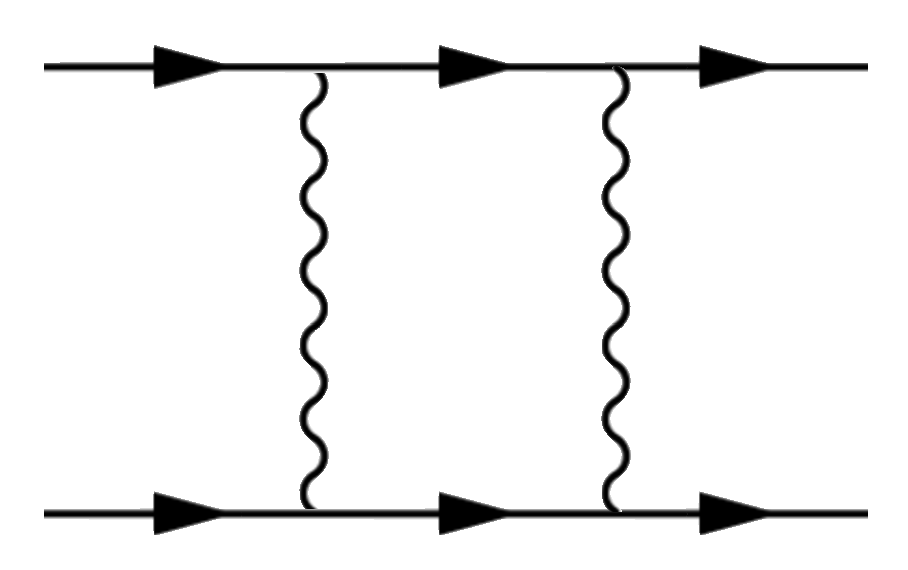
\includegraphics[scale=0.3]{imgs/NRQEDbox}
	\end{center}
	\vspace{-.6cm}
\caption{\small QEDにおける1ループ・ダイアグラムの例。} \label{fig:NRQEDbox}
\end{figure}


ここでNRQEDの議論に戻り、この考えを実際にどう実装するかを見てみよう。NRQEDで役割を果たす運動学的領域として、ポテンシャル領域とウルトラソフト領域の二つをすでに特定したが、実はさらにもう一つ考慮すべき領域がある。例えば、図\eqref{fig:NRQEDbox}に示したQEDのループ・ダイアグラムを考えよう。重心系で計算し、外線のフェルミオンがすべて非相対論的である状況に関心を絞る。全体にかかる定数因子を除くと、このループ・ダイアグラムは次の積分に等しい。
%
{\allowdisplaybreaks[0]\begin{align}
	& \int \frac{d^4 k}{(2\pi)^4} \,  N \, \frac{1}{k_0^2 - \vec{k}^{ 2} + i \epsilon } \, \frac{1}{(p_0 +k_0 - p_0')^2- (\vec p + \vec k - \vec{p}^{\,\prime})^2+ i \epsilon } \nonumber \\ 
	& \qquad \qquad \qquad \qquad \frac{1}{(p_0-k_0)^2 - (\vec p + \vec k)^2 - m^2 + i \epsilon } \, \frac{1}{(p_0+k_0)^2 - (\vec p + \vec k)^2- m^2 + i \epsilon   }, 
\end{align}}
%
ここで、$\pm \vec p$（$\pm \vec p^{\, \prime}$）は入射粒子（出射粒子）の3運動量であり、$N$は運動量の解析関数で、この議論では役割を果たさない。フェルミオンの運動エネルギー$E = p^0 - m$を用いて被積分関数を書き換え、記法を簡単にするために$i\epsilon$の因子を省くと便利である。その結果は次のとおりである。
%
\begin{align}
	& \int \frac{d^4 k}{(2\pi)^4} \,  N \, \frac{1}{k_0^2 - \vec{k}^{ 2} + i \epsilon } \, \frac{1}{(E - E' +k^0)^2- (\vec p + \vec k - \vec{p}^{\,\prime})^2+ i \epsilon } \nonumber \\ 
	& \qquad \qquad \qquad \qquad \qquad \qquad \frac{1}{E^2 - 2E k^0 - (\vec p + \vec k)^2 + i \epsilon } \, \frac{1}{E^2 + 2 E k^0 - (\vec p + \vec k)^2+ i \epsilon   }.
\end{align}
%
先ほどの議論によれば、被積分関数の任意の極の位置は、考慮すべき運動学的領域に対応する。$E, E' \sim mv^2$、$p, p' \sim mv$なので、第2の伝播関数は$(k^0, \vec k) \sim (mv, mv)$に極をもつ。この領域を\emph{ソフト}領域と呼ぶ。光子内線がソフトな4運動量を運ぶときには、エネルギー保存により、フェルミオン内線も同様でなければならないことに注意しよう。ソフト領域が必要となるのは、量子ループを考慮するときだけである。実際、\emph{古典的}な重力束縛状態を扱う非相対論的一般相対論（NRGR）~\cite{Goldberger:2007hy,Porto:2016pyg}では、この領域は何の役割も果たさない。

NRQEDで速度展開を系統的に実装するには、ソフト、ポテンシャル、ウルトラソフトの三つの領域で十分であることが分かる。このため、場$\psi$と$A^\mu$を次のように分解する。
%
\begin{subequations}\label{psi A decomposition}
\begin{align} 
	\psi &= \psi_{\rm S} + \psi_{\rm P} \\ 
	A^\mu &= A^\mu_{\rm S} + A^\mu_{\rm P} + A^\mu_{\rm U},
\end{align}
\end{subequations}
%
ここで、添字は対応する領域を表している。ウルトラソフトなフェルミオンを導入する必要がないことに注意しよう。上で導入したさまざまな場の間の相互作用は、$\mathcal{O} (mv^2)$の精度でエネルギーと運動量を保存しなければならない。ソフト領域とポテンシャル領域の場は$\mathcal{O}(mv)$のエネルギーまたは運動量をもつため、この段階では、それをどう実装するかは明らかでない。さらに、異なる領域の場の間の相互作用について、どのようにパワーカウンティングを行うべきかも明らかでない。積分測度$d^4x$は、どのようにスケールすべきなのだろうか。これらの問題に対処するため、ソフト場とポテンシャル場の位相を再定義し、$\mathcal{O}(mv)$の位相を取り出すことができる。
%
{\allowdisplaybreaks[0]\begin{subequations} \label{NRQED rephasing}
\begin{align}
	\psi_{\rm S} (x) &= \sum_p e^{i p \cdot x} \, \psi_{{\rm S}, p} (x) \\
	A_{\rm S}^\mu (x) &= \sum_p e^{i p \cdot x} \, A_{{\rm S}, p}^\mu (x) \\
	\psi_{\rm P} (x) &= \sum_{\vec p} e^{i \vec p \cdot \vec x} \, \psi_{{\rm P}, \vec p} \, (x) \\
	A_{\rm P}^\mu (x) &= \sum_{\vec p} e^{i \vec p \cdot \vec x} \, A_{{\rm P}, \vec p}^\mu \, (x) . 
\end{align}
\end{subequations}}
% 
ソフト場からは4運動量を、ポテンシャル場からは3運動量を取り出したことに注意しよう。上で述べた手順は、複数の領域の存在を考慮する必要があることを除けば、式\eqref{Psi tilde def}でフェルミオン場$\psi$を多くの場$\psi_{\vec p_F}$の和として表したときの手順と大きくは違わない。なお、ソフト場とポテンシャル場からソフトな位相を取り出すことは、ある種の多重極展開と考えることもできる~\cite{Labelle:1996en,Grinstein:1997gv}。ウルトラソフト場は、ソフト場とポテンシャル場の長波長での振る舞いしか探れないので、これは直観的にも理解できる。

\begin{table}[t!]
  \begin{center}
    \caption{NRQEDの場とその性質。}
    \label{tab: NRQED}
    \vspace{.4cm}
    \begin{tabular}{cccc}
    	\toprule
      \textbf{領域} & \textbf{場} & \textbf{スケーリング} & \textbf{伝播関数} \\
      	\midrule
      ソフト & $\begin{array}{c}
      		\psi_{{\rm S},  p} \\
      		A_{{\rm S}, p}^\mu 
      	\end{array}$ \vspace{.2cm} & $\begin{array}{l}
      		v^{3/2} \\
      		v 
      	\end{array}$ & $\begin{array}{c}
      		 i /(p^0 - i \epsilon) \\
      		-i \eta^{\mu\nu} / (p^{\, 2} - i \epsilon)
      	\end{array}$ \\
      	\midrule
      ポテンシャル & $\begin{array}{c}
      		\psi_{{\rm P}, \vec p} \\
      		A_{{\rm P}, \vec p}^\mu 
      	\end{array}$ \vspace{.2cm} & $\begin{array}{l}
      		v^{3/2} \\
      		v^{3/2}
      	\end{array}$ & $\begin{array}{c}
      		 i /(k^0 - \vec{p}^{\, 2}/2m + i \epsilon) \\
      		-i \eta^{\mu\nu} / (\vec{p}^{\, 2}  - i \epsilon)
      	\end{array}$ \\
      	\midrule
      ウルトラソフト & $A_{{\rm U}}^\mu$ & $\!\!\!\! v^2$ & $-i \eta^{\mu\nu}/(k^2-i\epsilon)$ \\
      \bottomrule
    \end{tabular}
  \end{center}
\end{table}

式\eqref{psi A decomposition}と\eqref{NRQED rephasing}を有効作用\eqref{NRQED action}に代入すれば、場$\psi_{{\rm S}, p}, \psi_{{\rm P}, \vec p}, A_{{\rm S}, p}^\mu, A_{{\rm P}, \vec p}^\mu \, ,$および$A_{{\rm U}}^\mu$の支配的な運動項と、それらの相互作用を導ける。これらの場に含まれるのは、残余のエネルギーと運動量が$\mathcal{O}(mv^2)$であるFourierモードだけなので、$\mathcal{O}(mv^2)$の精度での4運動量保存は自動的に保証される。さらに、積分測度の適切なスケーリングは、今や明らかに$d^4x \sim 1/v^8$である。すると、各場が$v$に応じてどうスケールするかを求め、伝播関数を計算することは容易である。結果を表\ref{tab: NRQED}にまとめた。ここでは、ソフトな運動量、すなわちラベルとしての運動量を$p$で、ウルトラソフトな運動量、すなわち残余運動量を$k$で表している。特に、ウルトラソフトなゲージ場は偏微分と同じようにスケールし、どちらも$\mathcal{O} (mv^2)$であることに注意しよう。したがって、これらを用いて、一様にスケールする共変微分$D_\mu = \partial_\mu - i e A_\mu^{\rm U}$を構成できる。
 
%
\begin{eBox}
%
{\bf 演習4.8：}表\ref{tab: NRQED}にまとめた結果を導け。
\end{eBox}
% 
NRQEDのすべてのFeynman則や実際の応用を詳しく説明することは、領域展開法の導入を主目的としたこの節の範囲を超える。詳しくは、次の節に挙げる文献を参照してほしい。
  



\subsectionlink{さらに学ぶための文献}



Fermi液体のEFTに関する標準的な文献は、PolchinskiのTASI講義録~\cite{Polchinski:1992ed}である。繰り込み群に基づく、有限密度フェルミオンのより網羅的な扱いについては、文献~\cite{Shankar:1993pf}を参照されたい。ヘリウム3の超流動に関する初期の教育的なレビューとして、文献~\cite{Leggett:1975te}がある。束縛状態の研究にNRQEDを用いることが最初に提唱されたのは、文献~\cite{Caswell:1985ui}である。非相対論的ゲージ理論のパワーカウンティングに伴う複雑さの大部分は、非相対論的QCD（NRQCD）の文脈で整理されてきた。NRQCDの詳細については、例えば文献~\cite{Rothstein:2003mp,Griesshammer:1997wz}を参照されたい。また、NRQEDに基づくLambシフトの計算も、文献~\cite{Rothstein:2003mp}にある。

\newpage


\section*{謝辞}


本講義を行う機会を与えてくださった第2回Joint ICTP-Trieste/ICTP-SAIFR school on Particle Physicsの主催者、Enrico Bertuzzo、Joan Elias Mir\'o、Rogerio Rosenfeld、Giovanni Villadoroに感謝する。また、刺激的な議論を交わしてくださったすべての参加者と他の講師にも感謝する。本講義録の準備にあたっては、この主題に関する多くの優れたレビューを読むことで多大な恩恵を受けた。その大部分は、適切な箇所で引用している。また、有益な議論と本講義録の初期稿へのコメントをくださったAngelo Esposito、Walter Goldberger、Garrett Goon、Alberto Nicolis、Rachel Rosen、Adam Solomon、そして特にIra Rothsteinに感謝する。本研究は、National Science Foundationの助成金No. PHY-1915611による支援を一部受けた。


\clearpage
\renewcommand{\refname}{\hyperlink{toc}{参考文献}}
\bibliographystyle{utphys}
\bibliography{ref}
\end{fmffile}
\end{document}
